\PassOptionsToPackage{table}{xcolor}
\documentclass{beamer}

% xcolor and define colors -------------------------
\usepackage[table]{xcolor}

% https://www.viget.com/articles/color-contrast/
\definecolor{purple}{HTML}{5601A4}
\definecolor{navy}{HTML}{0D3D56}
\definecolor{ruby}{HTML}{9a2515}
\definecolor{alice}{HTML}{107895}
\definecolor{daisy}{HTML}{EBC944}
\definecolor{coral}{HTML}{F26D21}
\definecolor{kelly}{HTML}{829356}
\definecolor{cranberry}{HTML}{E64173}
\definecolor{jet}{HTML}{131516}
\definecolor{asher}{HTML}{555F61}
\definecolor{slate}{HTML}{314F4F}

% Mixtape Sessions
\definecolor{picton-blue}{HTML}{00b7ff}
\definecolor{violet-red}{HTML}{ff3881}
\definecolor{sun}{HTML}{ffaf18}
\definecolor{electric-violet}{HTML}{871EFF}

% Main theme colors
\definecolor{accent}{HTML}{00b7ff}
\definecolor{accent2}{HTML}{871EFF}
\definecolor{gray100}{HTML}{f3f4f6}
\definecolor{gray800}{HTML}{1F292D}


% Beamer Options -------------------------------------

% Background
\setbeamercolor{background canvas}{bg = white}

% Change text margins
\setbeamersize{text margin left = 15pt, text margin right = 15pt}

% \alert
\setbeamercolor{alerted text}{fg = accent2}

% Frame title
\setbeamercolor{frametitle}{bg = white, fg = jet}
\setbeamercolor{framesubtitle}{bg = white, fg = accent}
\setbeamerfont{framesubtitle}{size = \small, shape = \itshape}

% Block
\setbeamercolor{block title}{fg = white, bg = accent2}
\setbeamercolor{block body}{fg = gray800, bg = gray100}

% Title page
\setbeamercolor{title}{fg = gray800}
\setbeamercolor{subtitle}{fg = accent}

%% Custom \maketitle and \titlepage
\setbeamertemplate{title page}
{
    %\begin{centering}
        \vspace{20mm}
        {\Large \usebeamerfont{title}\usebeamercolor[fg]{title}\inserttitle}\\
        {\large \itshape \usebeamerfont{subtitle}\usebeamercolor[fg]{subtitle}\insertsubtitle}\\ \vspace{10mm}
        {\insertauthor}\\
        {\color{asher}\small{\insertdate}}\\
    %\end{centering}
}

% Table of Contents
\setbeamercolor{section in toc}{fg = accent!70!jet}
\setbeamercolor{subsection in toc}{fg = jet}

% Button
\setbeamercolor{button}{bg = accent}

% Remove navigation symbols
\setbeamertemplate{navigation symbols}{}

% Table and Figure captions
\setbeamercolor{caption}{fg=jet!70!white}
\setbeamercolor{caption name}{fg=jet}
\setbeamerfont{caption name}{shape = \itshape}

% Bullet points

%% Fix left-margins
\settowidth{\leftmargini}{\usebeamertemplate{itemize item}}
\addtolength{\leftmargini}{\labelsep}

%% enumerate item color
\setbeamercolor{enumerate item}{fg = accent}
\setbeamerfont{enumerate item}{size = \small}
\setbeamertemplate{enumerate item}{\insertenumlabel.}

%% itemize
\setbeamercolor{itemize item}{fg = accent!70!white}
\setbeamerfont{itemize item}{size = \small}
\setbeamertemplate{itemize item}[circle]

%% right arrow for subitems
\setbeamercolor{itemize subitem}{fg = accent!60!white}
\setbeamerfont{itemize subitem}{size = \small}
\setbeamertemplate{itemize subitem}{$\rightarrow$}

\setbeamertemplate{itemize subsubitem}[square]
\setbeamercolor{itemize subsubitem}{fg = jet}
\setbeamerfont{itemize subsubitem}{size = \small}


% Special characters

\usepackage{collectbox}

\makeatletter
\newcommand{\mybox}{%
    \collectbox{%
        \setlength{\fboxsep}{1pt}%
        \fbox{\BOXCONTENT}%
    }%
}
\makeatother





% Links ----------------------------------------------

\usepackage{hyperref}
\hypersetup{
  colorlinks = true,
  linkcolor = accent2,
  filecolor = accent2,
  urlcolor = accent2,
  citecolor = accent2,
}


% Line spacing --------------------------------------
\usepackage{setspace}
\setstretch{1.1}


% \begin{columns} -----------------------------------
\usepackage{multicol}


% Fonts ---------------------------------------------
% Beamer Option to use custom fonts
\usefonttheme{professionalfonts}

% \usepackage[utopia, smallerops, varg]{newtxmath}
% \usepackage{utopia}
\usepackage[sfdefault,light]{roboto}

% Small adjustments to text kerning
\usepackage{microtype}



% Remove annoying over-full box warnings -----------
\vfuzz2pt
\hfuzz2pt


% Table of Contents with Sections
\setbeamerfont{myTOC}{series=\bfseries, size=\Large}
\AtBeginSection[]{
        \frame{
            \frametitle{Roadmap}
            \tableofcontents[current]
        }
    }


% Tables -------------------------------------------
% Tables too big
% \begin{adjustbox}{width = 1.2\textwidth, center}
\usepackage{adjustbox}
\usepackage{array}
\usepackage{threeparttable, booktabs, adjustbox}

% Fix \input with tables
% \input fails when \\ is at end of external .tex file
\makeatletter
\let\input\@@input
\makeatother

% Tables too narrow
% \begin{tabularx}{\linewidth}{cols}
% col-types: X - center, L - left, R -right
% Relative scale: >{\hsize=.8\hsize}X/L/R
\usepackage{tabularx}
\newcolumntype{L}{>{\raggedright\arraybackslash}X}
\newcolumntype{R}{>{\raggedleft\arraybackslash}X}
\newcolumntype{C}{>{\centering\arraybackslash}X}

% Figures

% \imageframe{img_name} -----------------------------
% from https://github.com/mattjetwell/cousteau
\newcommand{\imageframe}[1]{%
    \begin{frame}[plain]
        \begin{tikzpicture}[remember picture, overlay]
            \node[at = (current page.center), xshift = 0cm] (cover) {%
                \includegraphics[keepaspectratio, width=\paperwidth, height=\paperheight]{#1}
            };
        \end{tikzpicture}
    \end{frame}%
}

% subfigures
\usepackage{subfigure}


% Highlight slide -----------------------------------
% \begin{transitionframe} Text \end{transitionframe}
% from paulgp's beamer tips
\newenvironment{transitionframe}{
    \setbeamercolor{background canvas}{bg=accent!40!black}
    \begin{frame}\color{accent!10!white}\LARGE\centering
}{
    \end{frame}
}


% Table Highlighting --------------------------------
% Create top-left and bottom-right markets in tabular cells with a unique matching id and these commands will outline those cells
\usepackage[beamer,customcolors]{hf-tikz}
\usetikzlibrary{calc}
\usetikzlibrary{fit,shapes.misc}

% To set the hypothesis highlighting boxes red.
\newcommand\marktopleft[1]{%
    \tikz[overlay,remember picture]
        \node (marker-#1-a) at (0,1.5ex) {};%
}
\newcommand\markbottomright[1]{%
    \tikz[overlay,remember picture]
        \node (marker-#1-b) at (0,0) {};%
    \tikz[accent!80!jet, ultra thick, overlay, remember picture, inner sep=4pt]
        \node[draw, rectangle, fit=(marker-#1-a.center) (marker-#1-b.center)] {};%
}

\usepackage{breqn} % Breaks lines

\usepackage{amsmath}
\usepackage{mathtools}

\usepackage{pdfpages} % \includepdf

\usepackage{listings} % R code
\usepackage{verbatim} % verbatim

% Video stuff
\usepackage{media9}

% packages for bibs and cites
\usepackage{natbib}
\usepackage{har2nat}
\newcommand{\possessivecite}[1]{\citeauthor{#1}'s \citeyearpar{#1}}
\usepackage{breakcites}
\usepackage{alltt}

% Setup math operators
\DeclareMathOperator{\E}{E} \DeclareMathOperator{\tr}{tr} \DeclareMathOperator{\se}{se} \DeclareMathOperator{\I}{I} \DeclareMathOperator{\sign}{sign} \DeclareMathOperator{\supp}{supp} \DeclareMathOperator{\plim}{plim}
\DeclareMathOperator*{\dlim}{\mathnormal{d}\mkern2mu-lim}
\newcommand\independent{\protect\mathpalette{\protect\independenT}{\perp}}
   \def\independenT#1#2{\mathrel{\rlap{$#1#2$}\mkern2mu{#1#2}}}
\newcommand*\colvec[1]{\begin{pmatrix}#1\end{pmatrix}}

\newcommand{\myurlshort}[2]{\href{#1}{\textcolor{gray}{\textsf{#2}}}}


\begin{document}

\imageframe{./lecture_includes/slide_banner.pdf}


% ---- Content ----




\section{Differential timing or $G \times T$} 

\subsection{Bacon Decomposition}

\begin{frame}{Estimator Selection for Differential Timing}

\begin{itemize}
\item What if there had not been just one treatment cohort, but several? 
\item Think of there being three options with differential timing 
	\begin{enumerate}
	\item Traditional twoway fixed effects (TWFE)
	\item Aggregating ATT(g,t) using Callaway and Sant'Anna or Sun and Abraham
	\item Imputation using Borusyak, Jaravel and Speiss (BJS), Gardner or Wooldridge (Kyle will discuss these)
	\end{enumerate}
\item  Let's review now the differential timing literature with an aim to making a decision among them
\end{itemize}

\end{frame}

\begin{frame}{Five approaches we will study}

\begin{enumerate}
\item Twoway fixed effects (Goodman-Bacon 2021)
\item Callaway and Sant'Anna (2021), or CS
\item Sun and Abraham (2021), or SA
\item de Chaisemartin and D'Haultfouielle (2020), or dCDH
\item Borusywak, Jaravel and Spiess (2024), or BJS (Kyle)
\end{enumerate}
\end{frame}

\begin{frame}{Choosing between them}

\begin{itemize}
\item First goal is to understand them, their assumptions, their mechanics and their code
\item Second goal is to present a simple criteria for selecting between them so that you aren't "cherry picking your diff-in-diff"
\end{itemize}

\end{frame}




\begin{frame}{Twoway fixed effects}

\begin{itemize}
\item When working with panel data, the so-called TWFE estimator is the workhorse estimator
\item It's easy to implement, handles time-varying treatments, has a relatively straightforward interpretation under constant treatment effects, standard errors are easy to calculate and understand
\item Interpretation is more complicated with heterogenous treatment effects
\end{itemize}

\end{frame}




\begin{frame}{Discussion of estimate}


$$Y_{ist} = \beta_0 + \delta D_{ist} + \tau_t + \sigma_s + \varepsilon_{ist}$$


\begin{itemize}
\item If you estimate with OLS with differential timing, what does $\widehat{\delta}$ correspond to?
\item It is a weighted average of all possible ``four averages and three subtractions'' 
\item So similar to the 2x2 regression, except the coefficient is a weighted average over several -- including one that we should have avoided all along

\end{itemize}

\end{frame}




\begin{frame}{$K^2$ distinct DDs}

Let's look at 3 timing groups (a, b and c) and one untreated group (U).  With 3 timing groups, there are 9 2x2 DDs.  Here they are:


\begin{center}
\begin{tabular}{c|c|c}
\multicolumn{1}{l}{} &
\multicolumn{1}{l}{} &
\multicolumn{1}{l}{} \\
\midrule
a to b & b to a & c to a \\
a to c & b to c & c to b \\
a to U & b to U & c to U \\
\midrule
\end{tabular}
\end{center}

\bigskip

Let's return to a simpler example with only two groups -- a $k$ group treated at $t_k^*$ and an $l$ treated at $t_l^*$ plus an never-treated group called the $U$ untreated group
\end{frame} 


\begin{frame}{Terms and notation}

\begin{itemize}
\item Let there be two treatment groups ($k,l$) and one untreated group ($U$)
\item $k,l$ define the groups based on when they receive treatment (differently in time) with k receiving it earlier than $l$
\item Denote $\overline{D}_k$ as the share of time each group spends in treatment status
\item Denote $\widehat{\delta}_{jb}^{2x2}$ as the canonical $2\times 2$ DD estimator for groups $j$ and b where $j$ is the treatment group and $b$ is the comparison group
\end{itemize}

\end{frame}


\imageframe{./lecture_includes/bacon_goodman_2.png}



\begin{frame}[plain]
$$\widehat{\delta}^{2x2}_{kU} = \bigg ( \overline{y}_k^{post(k)} - \overline{y}_k^{pre(k)} \bigg ) - \bigg ( \overline{y}_U^{post(k)} - \overline{y}_U^{pre(k)} \bigg ) $$
	\begin{figure}
	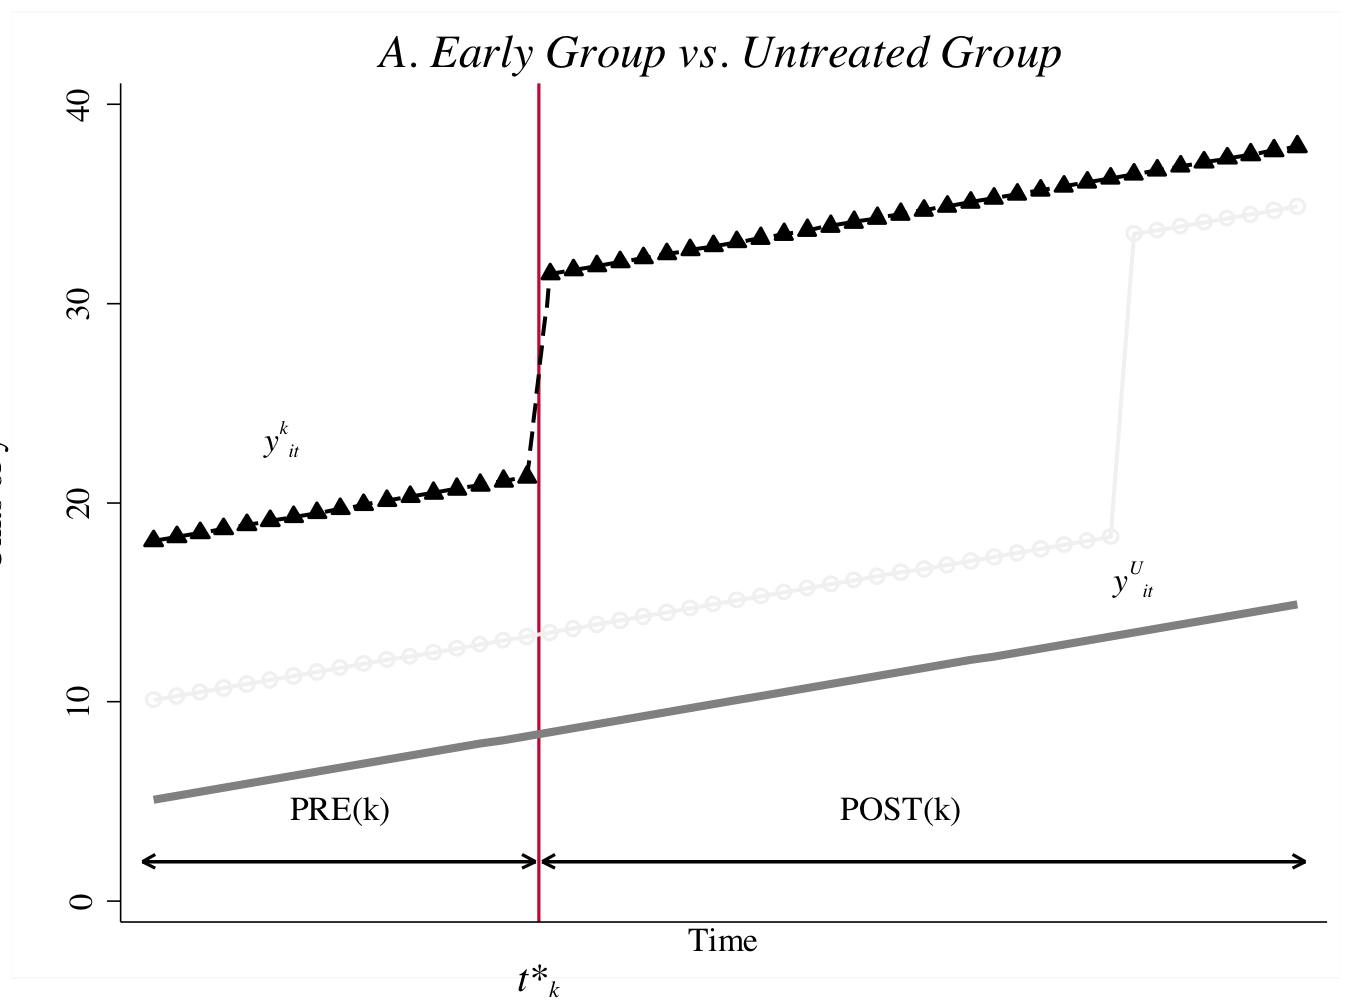
\includegraphics[scale=0.45]{./lecture_includes/bacon_goodman_3.png}
	\end{figure}

\end{frame}

\begin{frame}[plain]
$$\widehat{\delta}^{2x2}_{lU} = \bigg ( \overline{y}_l^{post(l)} - \overline{y}_l^{pre(l)} \bigg ) - \bigg ( \overline{y}_U^{post(l)} - \overline{y}_U^{pre(l)} \bigg ) $$
	\begin{figure}
	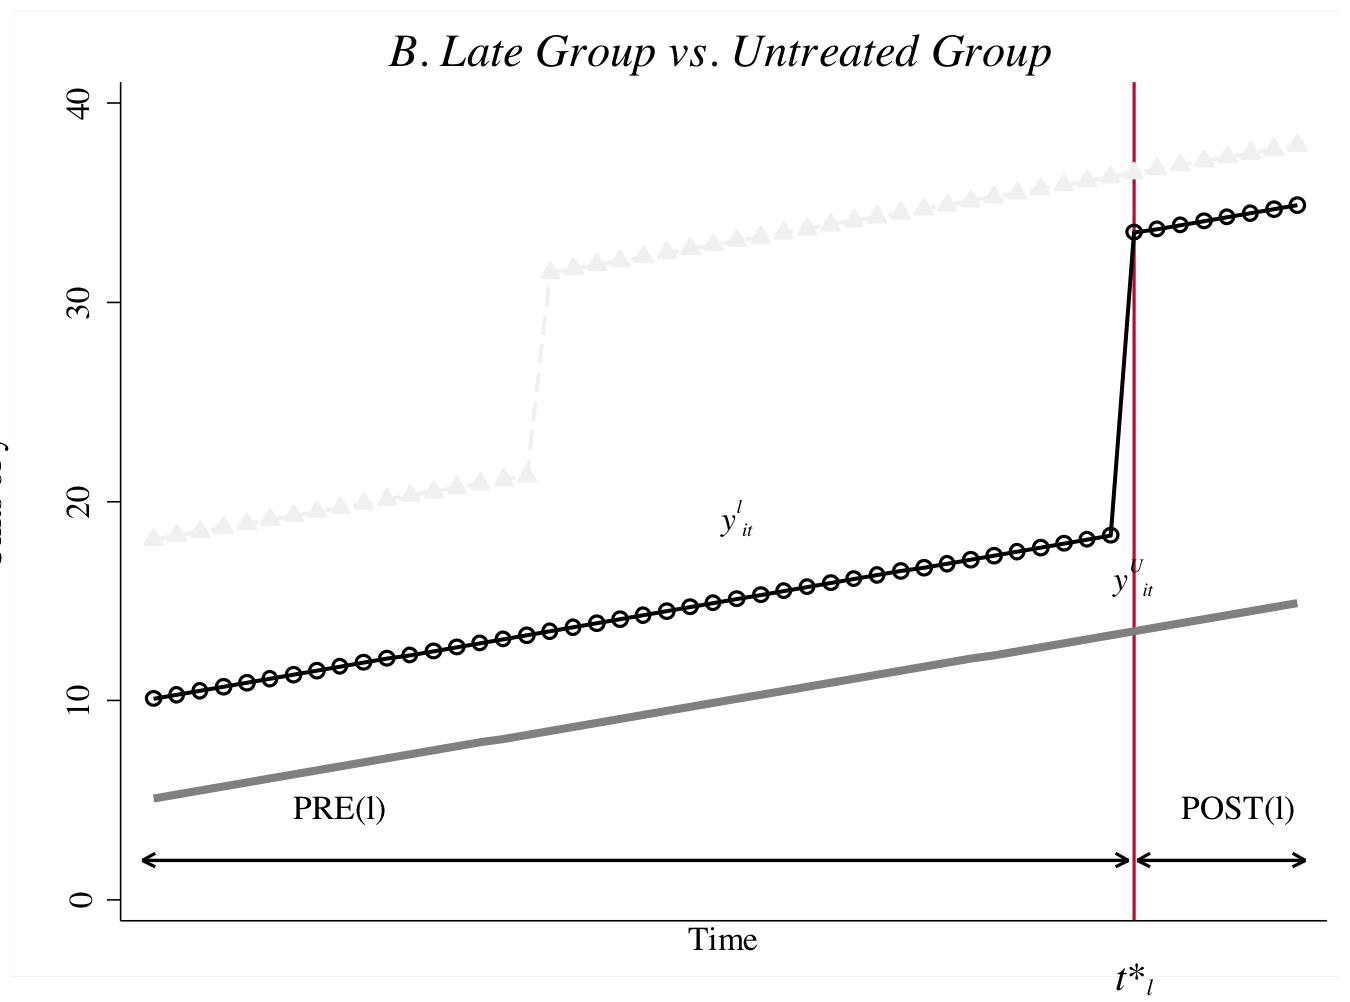
\includegraphics[scale=0.45]{./lecture_includes/bacon_goodman_4.png}
	\end{figure}

\end{frame}


\begin{frame}[plain]

$$\delta_{kl}^{2x2,k} = \bigg ( \overline{y}_k^{MID(k,l)} - \overline{y}_k^{Pre(k,l)} \bigg ) - \bigg ( \overline{y}_l^{MID(k,l)} - \overline{y}_l^{PRE(k,l)} \bigg ) $$

	\begin{figure}
	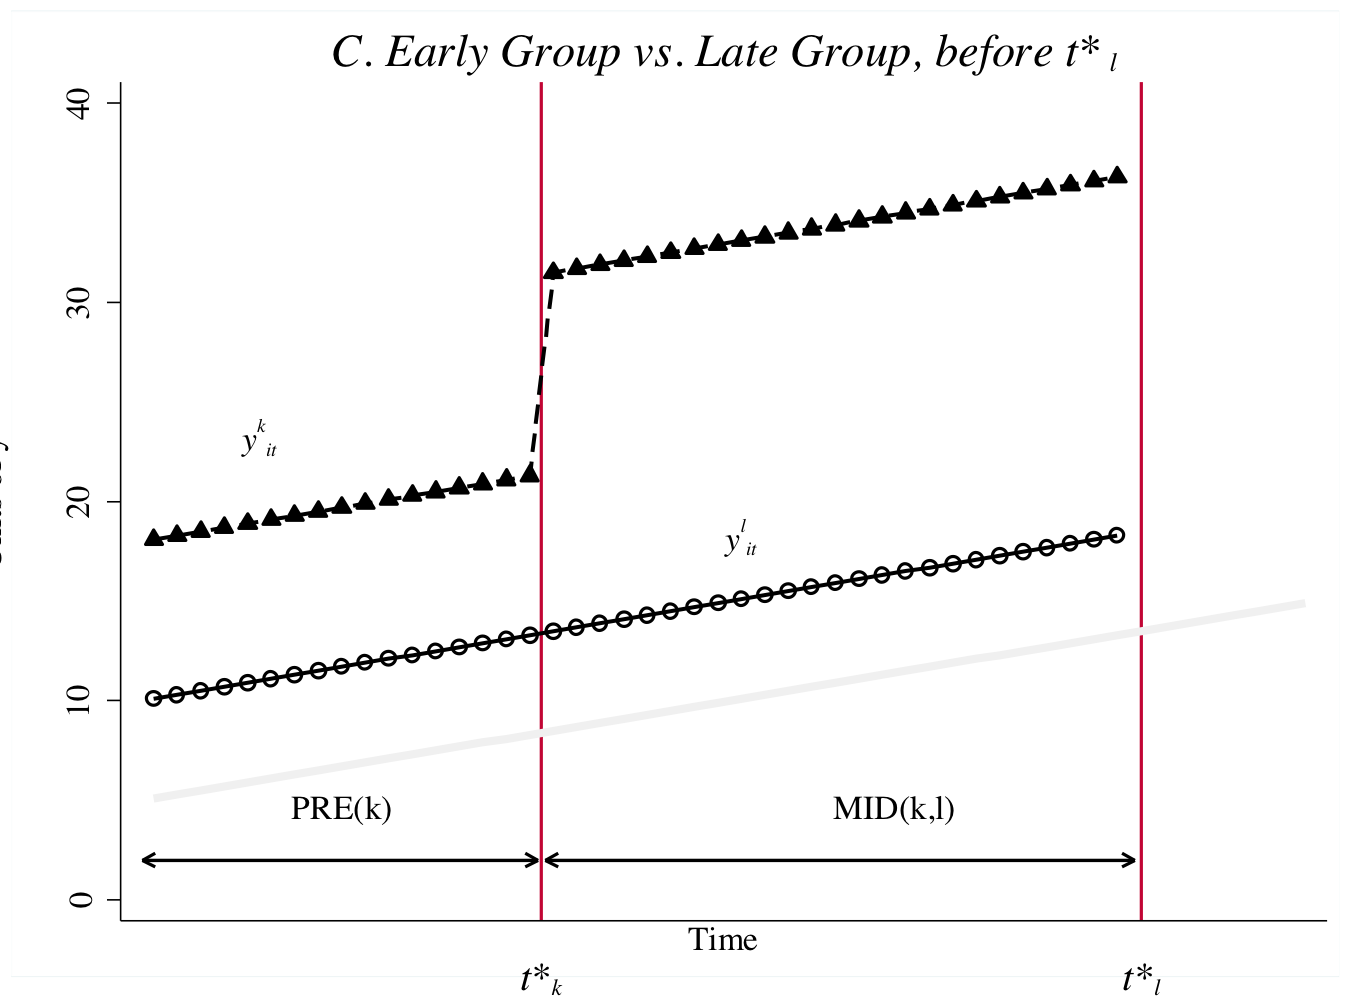
\includegraphics[scale=0.45]{./lecture_includes/bacon_goodman_6.png}
	\end{figure}

\end{frame}

\begin{frame}[plain]
$$\delta_{lk}^{2x2,l} = \bigg ( \overline{y}_l^{POST(k,l)} - \overline{y}_l^{MID(k,l)} \bigg ) - \bigg ( \overline{y}_k^{POST(k,l)} - \overline{y}_k^{MID(k,l)} \bigg ) $$

	\begin{figure}
	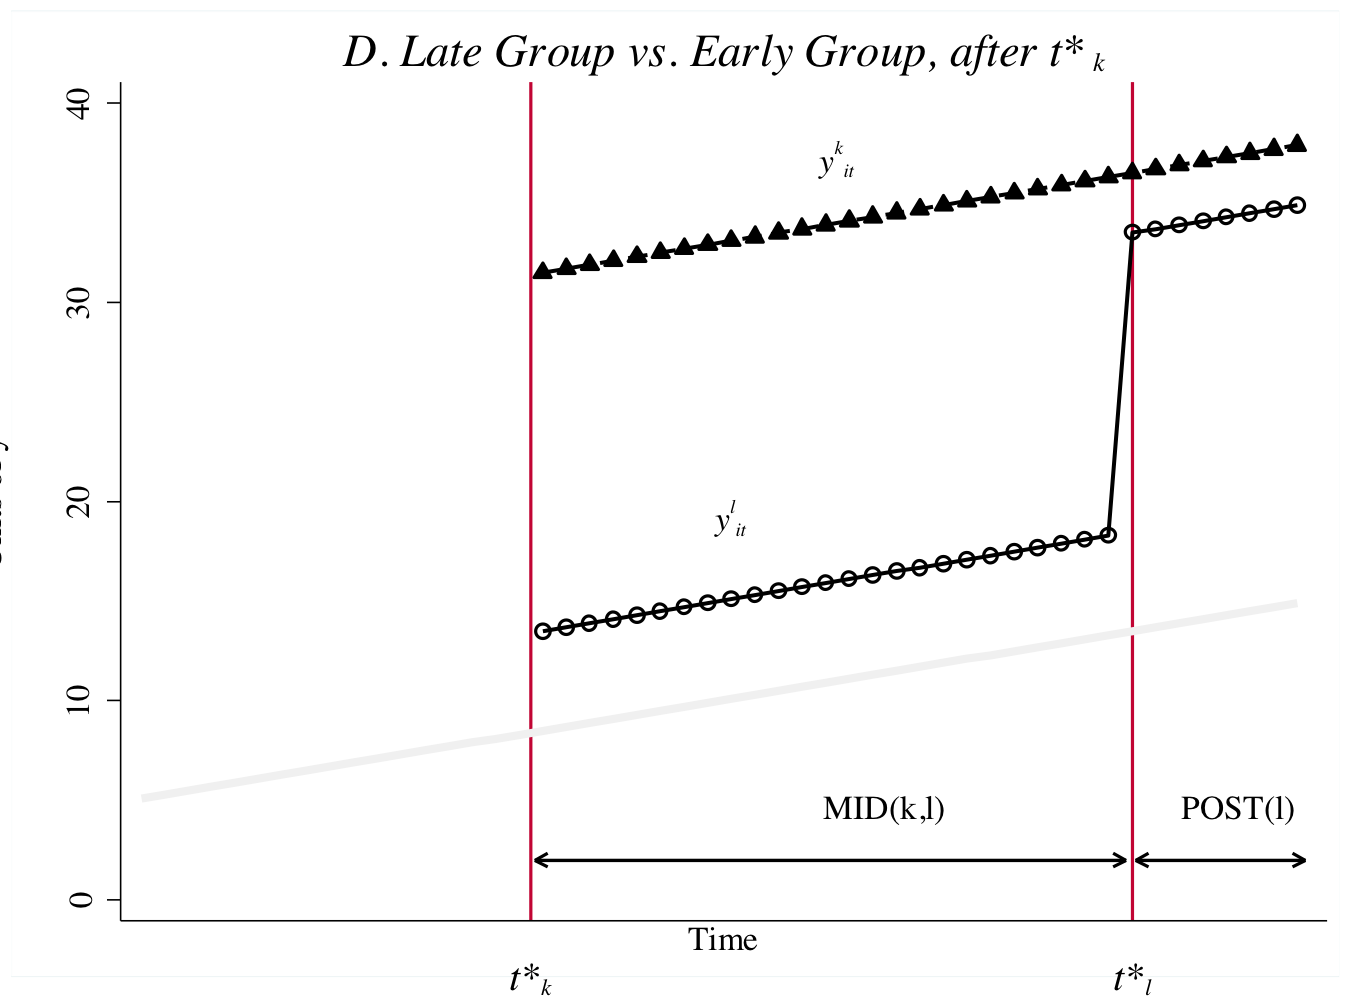
\includegraphics[scale=0.4]{./lecture_includes/bacon_goodman_7.png}
	\end{figure}

\end{frame}


	

\begin{frame}{Bacon decomposition}

$$Y_{ist} = \beta_0 + \delta D_{ist} + \tau_t + \sigma_s + \varepsilon_{ist}$$


TWFE estimate of $\widehat{\delta}$ is equal to a weighted average over all group 2x2 (of which there are 4 in this example)
\begin{eqnarray*}	
\widehat{\delta}^{TWFE} = \sum_{k \neq U} s_{kU}\widehat{\delta}_{kU}^{2x2} + \sum_{k \neq U} \sum_{l>k} s_{kl}  \bigg [ \mu_{kl}\widehat{\delta}_{kl}^{2x2,k} + (1-\mu_{kl}) \widehat{\delta}_{lk}^{2x2,l} \bigg]
\end{eqnarray*}where that first 2x2 combines the k compared to U and the l to U (combined to make the equation shorter)

\end{frame}
	


\begin{frame}{Third, the Weights}

 \begin{eqnarray*} s_{ku} &=& \frac{ n_k n_u \overline{D}_k (1- \overline{D}_k ) }{ \widehat{Var} ( \tilde{D}_{it} )} \\
s_{kl} &=& \frac{ n_k n_l (\overline{D}_k - \overline{D}_{l} ) ( 1- ( \overline{D}_k - \overline{D}_{l} )) }{\widehat{Var}(\tilde{D}_{it})} \\
\mu_{kl} &=& \frac{1 - \overline{D}_k }{1 - ( \overline{D}_k - \overline{D}_{l} )}
\end{eqnarray*}where $n$ refer to the panel group shares, $\overline{D}_k (1- \overline{D}_k )$, as well as $(\overline{D}_k - \overline{D}_{l} ) ( 1- ( \overline{D}_k - \overline{D}_{l} ))$ expressions refer to variance of treatment, and the final equation is the same for two timing groups.

\end{frame}

\begin{frame}{Weights discussion}

\begin{itemize}
\item Two things to note:
	\begin{itemize}
	\item More units in a group, the bigger its 2x2 weight is
	\item Group treatment variance weights up or down a group's 2x2
	\end{itemize}
\item Think about what causes the treatment variance to be as big as possible. Let's think about the $s_{ku}$ weights.
	\begin{itemize}
	\item $\overline{D}=0.1$. Then $0.1 \times 0.9 = 0.09$
	\item $\overline{D}=0.4$. Then $0.4 \times 0.6 =0.24$
	\item $\overline{D}=0.5$. Then $0.5 \times 0.5 = 0.25$
	\item $\overline{D}=0.6$. Then $0.6 \times 0.4 = 0.24$
	\end{itemize}
\item This means the weight on treatment variance is maximized for \emph{groups treated in middle of the panel}
\end{itemize}
\end{frame}

\begin{frame}{More weights discussion}

\begin{itemize}
\item But what about the ``treated on treated'' weights (i.e., $\overline{D}_k - \overline{D}_{l} $)  
\item Same principle as before - when the difference between treatment variance is close to 0.5, those 2x2s are given the greatest weight
\item For instance, say $t^*_k=0.15$ and $t^*_l=0.67$. Then $\overline{D}_k - \overline{D}_{l} = 0.52$.  And thus $0.52 \times 0.48 = 0.2496$.
\end{itemize}

\end{frame}


\begin{frame}{Summarizing TWFE centralities}

\begin{itemize}
\item Groups in the middle of the panel weight up their respective 2x2s via the variance weighting
\item Decomposition highlights the strange role of panel length when using TWFE
\item Different choices about panel length change both the 2x2 and the weights based on variance of treatment
\end{itemize}

\end{frame}




\begin{frame}{Back to TWFE}


$$Y_{ist} = \beta_0 + \delta D_{ist} + \tau_t + \sigma_s + \varepsilon_{ist}$$


\begin{itemize}

\item So we know that the estimate is a weighted average over all ``four averages and three subtractions'' but is that good or bad?
\item It's good if it's unbiased; it's bad if it isn't, and the decomposition doesn't tell us which unless we replace realized outcomes with potential outcomes
\item Bacon shows that TWFE estimate of $\delta$ needs two assumptions for unbiasedness:
	\begin{enumerate}
	\item variance weighted parallel trends are zero and 
	\item no dynamic treatment effects (not the case with 2x2)
	\end{enumerate}
\item Under those assumptions, TWFE estimator estimates the variance weighted ATT as a weighted average of all possible ATTs (not just weighted average of DiDs)

\end{itemize}

\end{frame}


\begin{frame}{Moving from 2x2s to causal effects and bias terms}

Let's start breaking down these estimators into their corresponding estimation objects expressed in causal effects and biases


\begin{eqnarray*}
\widehat{\delta}^{2x2}_{kU} &=& ATT_k{Post} + \Delta Y^0_k(Post(k),Pre(k)) - \Delta Y^0_U(Post(k),Pre) \\
\widehat{\delta}^{2x2}_{kl} &=& ATT_k(MID) + \Delta Y^0_k(MID,Pre) - \Delta Y^0_l(MID, Pre)
\end{eqnarray*}These look the same because you're always comparing the treated unit with an untreated unit (though in the second case it's just that they haven't been treated \emph{yet}). 

\end{frame}

\begin{frame}{The dangerous 2x2}

But what about the 2x2 that compared the late groups to the already-treated earlier groups? With a lot of substitutions we get:

\begin{eqnarray*}
\widehat{\delta}^{2x2}_{lk} &=& ATT_{l,Post(l)} + \underbrace{\Delta Y^0_l(Post(l),MID) - \Delta Y^0_k ( Post(l), MID)}_{\mathclap{\text{Parallel trends bias}}} \\
&& - \underbrace{(ATT_k(Post) - ATT_k(Mid))}_{\mathclap{\text{Heterogeneity bias!}}}
\end{eqnarray*}


\end{frame}

\begin{frame}{Substitute all this stuff into the decomposition formula}

\begin{eqnarray*}	
\widehat{\delta}^{TWFE} = \sum_{k \neq U} s_{kU}\widehat{\delta}_{kU}^{2x2} + \sum_{k \neq U} \sum_{l>k} s_{kl}  \bigg [ \mu_{kl}\widehat{\delta}_{kl}^{2x2,k} + (1-\mu_{kl}) \widehat{\delta}_{kl}^{2x2,l} \bigg]
\end{eqnarray*}where we will make these substitutions\begin{eqnarray*}
\widehat{\delta}_{kU}^{2x2} &=& ATT_k(Post) + \Delta Y_k^0(Post,Pre) - \Delta Y_U^0(Post, Pre) \\
\widehat{\delta}_{kl}^{2x2,k} &=& ATT_k(Mid) + \Delta Y_k^0(Mid,Pre) - \Delta Y_l^0(Mid, Pre) \\
\widehat{\delta}^{2x2,l}_{lk} &=& ATT_{l}Post(l) + \Delta Y^0_l(Post(l),MID) - \Delta Y^0_k ( Post(l), MID) \\
&&- (ATT_k(Post) - ATT_k(Mid))
\end{eqnarray*}Notice all those potential sources of biases! 

\end{frame}


\begin{frame}{Potential Outcome Notation}

\begin{eqnarray*}
p\text{ }lim\text{ } \widehat{\delta}^{TWFE}_{n\to\infty} &=& VWATT + VWPT - \Delta ATT
\end{eqnarray*}

\begin{itemize}
\item Notice the number of assumptions needed \emph{even} to estimate this very strange weighted ATT (which is a function of how you drew the panel in the first place). 
\item With dynamics, it attenuates the estimate (bias) and can even reverse sign depending on the magnitudes of what is otherwise effects in the sign in a reinforcing direction! 
\item Model can flip signs (does not satisfy a ``no sign flip property'')
\end{itemize}

\end{frame}






\begin{frame}{Simulated data}

\begin{itemize}
\item 1000 firms, 40 states, 25 firms per states, 1980 to 2009 or 30 years, 30,000 observations, four groups

\item I'll impose ``unit level parallel trends'', which is much stronger than we need (we only need average parallel trends)

\item Also no anticipation of treatment effects until treatment occurs but does \emph{not} guarantee homogenous treatment effects

\item Two types of situations: constant versus dynamic treatment effects
\end{itemize}
\end{frame}



\begin{frame}{Constant vs Dynamic Treatment Effects}
    \begin{columns}
        \column{0.5\linewidth}
        \centering
        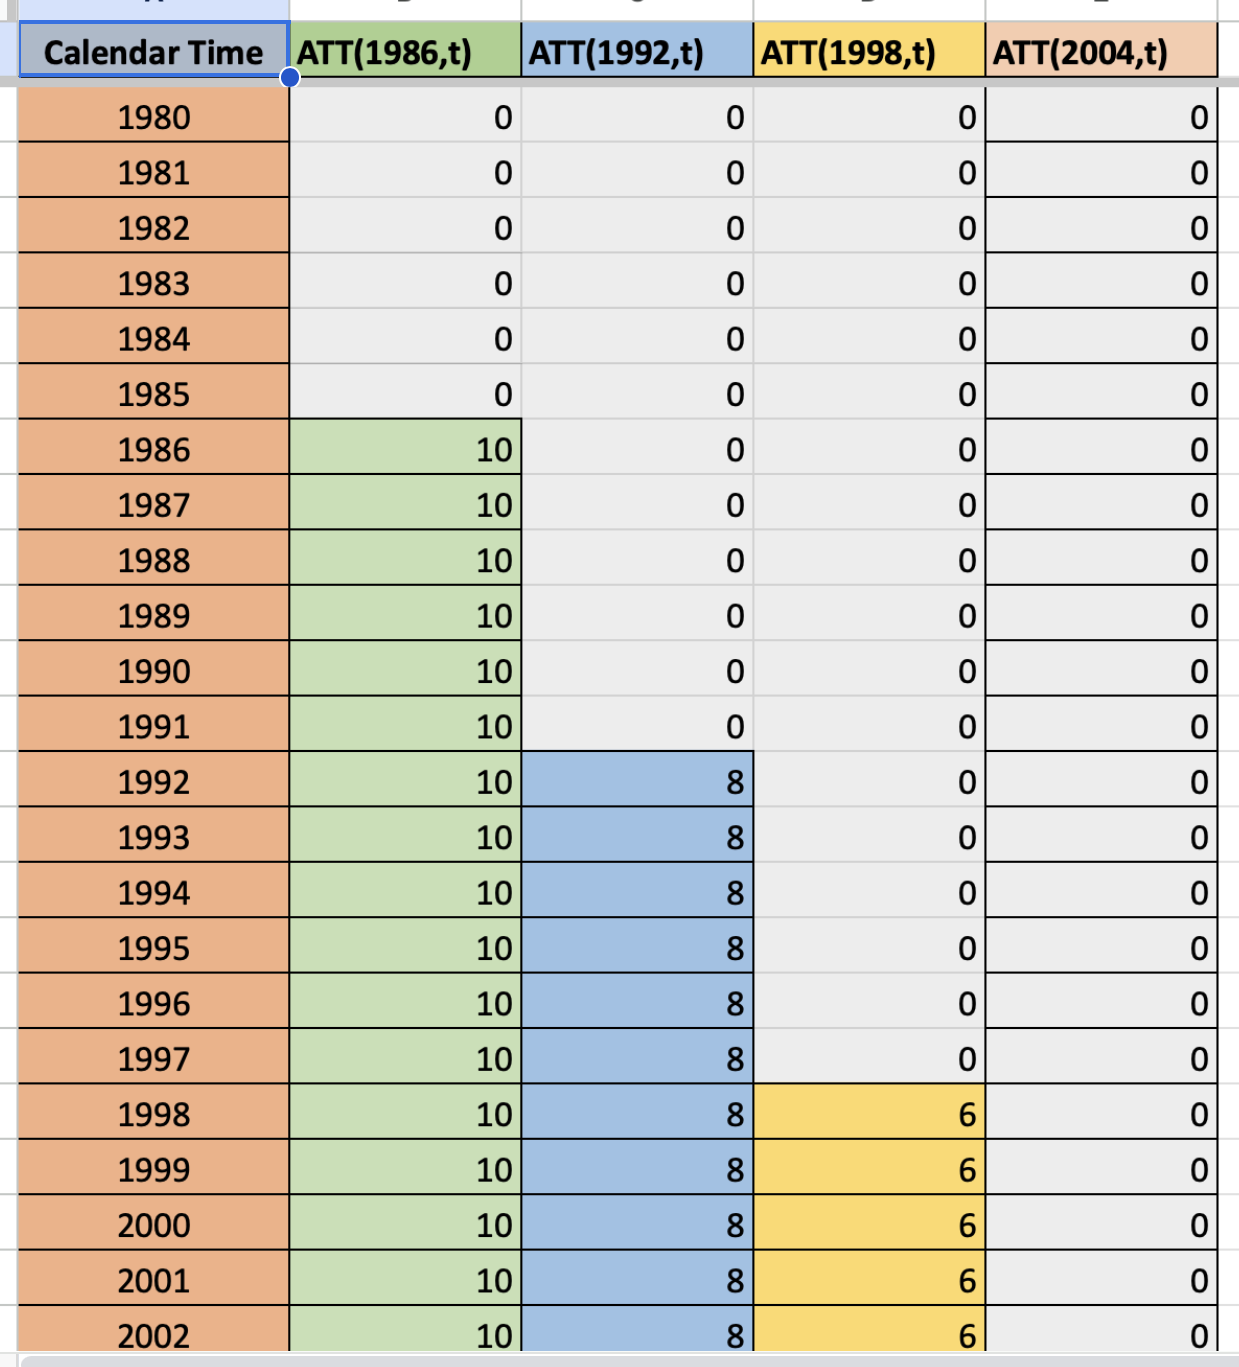
\includegraphics[height=6.5cm, width=5.5cm]{./lecture_includes/constant_te}

        \column{0.5\linewidth}
        \centering
        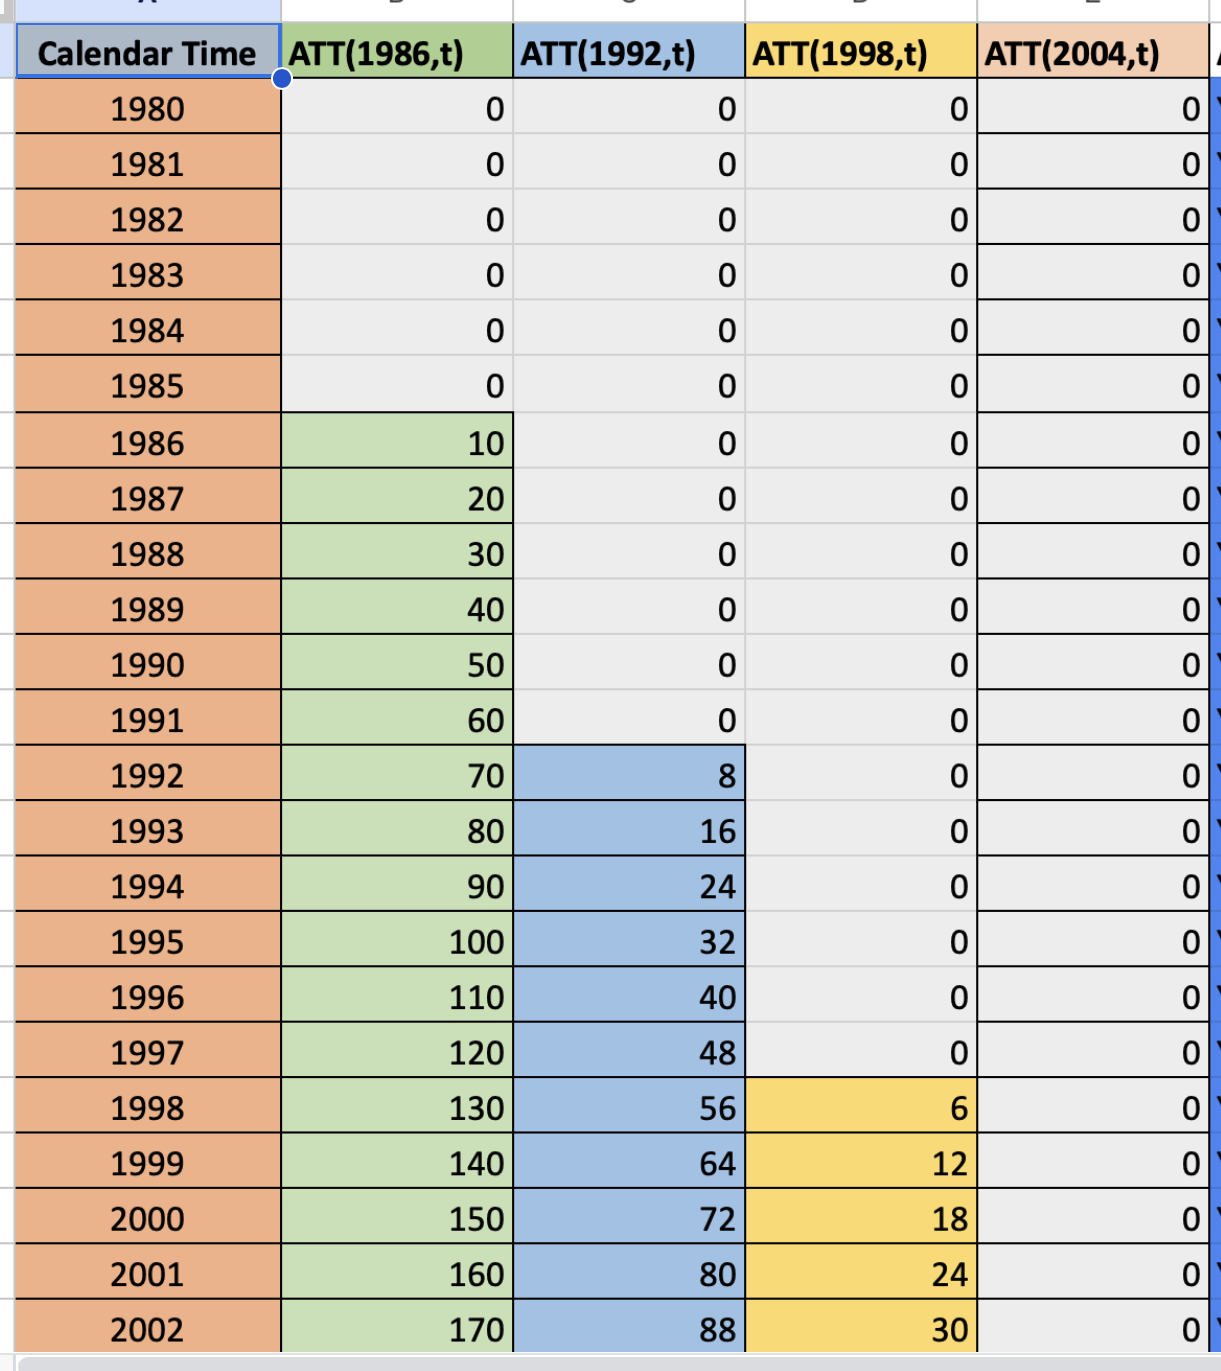
\includegraphics[height=6.5cm, width=5.5cm]{./lecture_includes/dynamic_te}
    \end{columns} 
\end{frame}



\begin{frame}{Group-time ATT}
       \begin{columns}
          \column{0.38\linewidth}
             \centering
             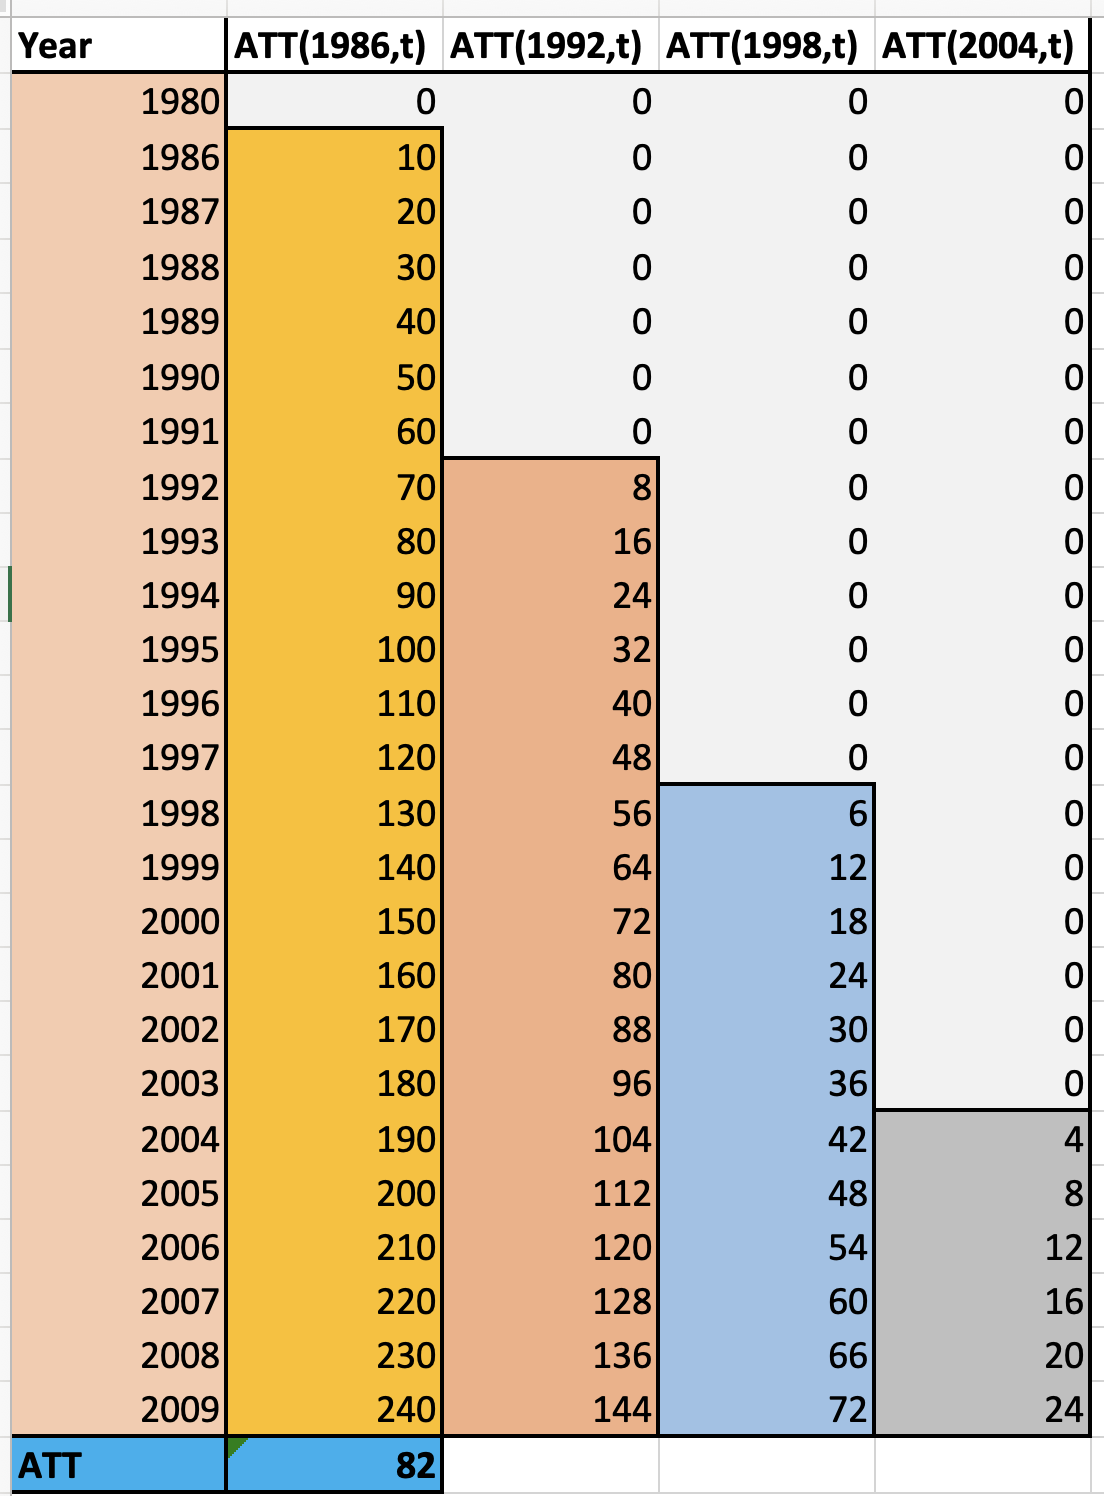
\includegraphics[height=6.5cm, width=5.5cm]{./lecture_includes/baker_attgt}
           \column{0.48\linewidth}
		\begin{itemize}
\item Heterogenous treatment effects across time and across groups
\item Cells are called ``group-time ATT'' (Callaway and Sant'Anna 2021) or ``cohort ATT'' (Sun and Abraham 2021)
\item ATT is weighted average of all cells and $+82$ with uniform weights $1/60$
		\end{itemize}
         \end{columns} 
    \end{frame}
    
    

\begin{frame}{Estimation}

\bigskip

Estimate the following equation using OLS:

$$Y_{ist} = \alpha_i + \gamma_t +\delta D_{it} + \varepsilon_{ist}$$


\begin{table}[htbp]\centering
\small
\caption{Estimating ATT with different models}
\begin{center}
\begin{tabular}{l*{5}{c}}
\hline
\multicolumn{1}{l}{\textbf{}}&
\multicolumn{1}{c}{\textbf{Truth}}&
\multicolumn{1}{c}{\textbf{(TWFE)}}&
\multicolumn{1}{c}{\textbf{(CS)}}&
\multicolumn{1}{c}{\textbf{(SA)}}&
\multicolumn{1}{c}{\textbf{(BJS)}}\\
\hline
$\widehat{ATT}$  & 82    & -6.69*** &&&\\
\hline
\end{tabular}
\end{center}
\end{table}

The sign flipped.  Why?  Because of \emph{extreme} dynamics (i.e., $- \Delta ATT$)

\end{frame}

\begin{frame}{Bacon decomposition}
\begin{table}[htbp]\centering
\small
\caption{Bacon Decomposition (TWFE $= -6.69$)}
\begin{center}
\begin{tabular}{l*{5}{c}}
\hline
\multicolumn{1}{l}{\textbf{DD Comparison}}&
\multicolumn{1}{l}{\textbf{Weight}}&
\multicolumn{1}{l}{\textbf{Avg DD Est}}\\
\hline
Earlier T vs. Later C  &     0.500   &       51.800 \\
Later T vs. Earlier C   &    0.500    &     -65.180 \\
\midrule
T $=$ Treatment; C$ =$ Comparison \\
$(0.5*51.8) + (0.5*-65.180) = -6.69$ \\
\hline
\end{tabular}
\end{center}
\end{table}

\bigskip

While large weight on the ``late to early 2x2'' is \emph{suggestive} of an issue, these would appear even if we had constant treatment effects

\end{frame}


\subsection{Callaway and Sant'Anna (CS)}


\begin{frame}{Reverse Engineering}

\begin{itemize}
\item Heckman (1990) showed that with noncompliance and heterogenous treatment effects, IV identified the ATE only in the most extreme case (when the instrument pushed everyone into treatment called "identification at infinity"
\item Imbens and Angrist (1994) showed that instrumental variables identified the "local average treatment effect" (LATE)
\item Note: they did not propose an IV estimator that would identify the ATE which was Heckman's point -- rather they "reverse engineered" what IV did
\end{itemize}

\end{frame}

\begin{frame}{Reverse Engineering}

\begin{itemize}
\item Reverse (or backwards) engineering is when someone takes a model, and simply shows what it means
\item The new diff-in-diff literature has many papers that did that -- the most commonly known being Goodman-Bacon (2021) and his "Bacon decomposition"
\item All Bacon did was take a particular twoway fixed effects regression specification and show it was equal to a variance weighted average of "all $2 \times 2$" calculations (some bad)
\item Bacon \textbf{did not} propose a solution just like Imbens and Angrist (1994) did not propose a solution -- reverse engineering is not "solutions oriented", per se

\end{itemize}

\end{frame}

\begin{frame}{Forward Engineering}

\begin{itemize}
\item When people design new estimators designed to overcome various problems, they are not reverse engineering -- they are \textbf{forward engineering}
\item Our next model is by Callaway and Sant'Anna (2021) and is an example of this 
\item They do not decompose what TWFE does (reverse engineering) but build a model that does not depend on as many assumptions
\end{itemize}

\end{frame}





\begin{frame}{Callaway and Sant'Anna 2021}

CS is a diff-in-diff estimator used with differential timing and a binary treatment that turns on (and stays on) to estimate smaller "building block" causal parameters called group-time $ATT(g,t)$ and is used in situations like these:

\begin{enumerate}
\item Treatment effects differ in the shortrun than the longrun
\item Treatment effects differ by time period
\item Treatment effects have different dynamics for different groups
\item In other words, \emph{unrestricted heterogenous treatment effects}
\end{enumerate}


\end{frame}




\begin{frame}{Group-time ATT}
       \begin{columns}
          \column{0.38\linewidth}
             \centering
             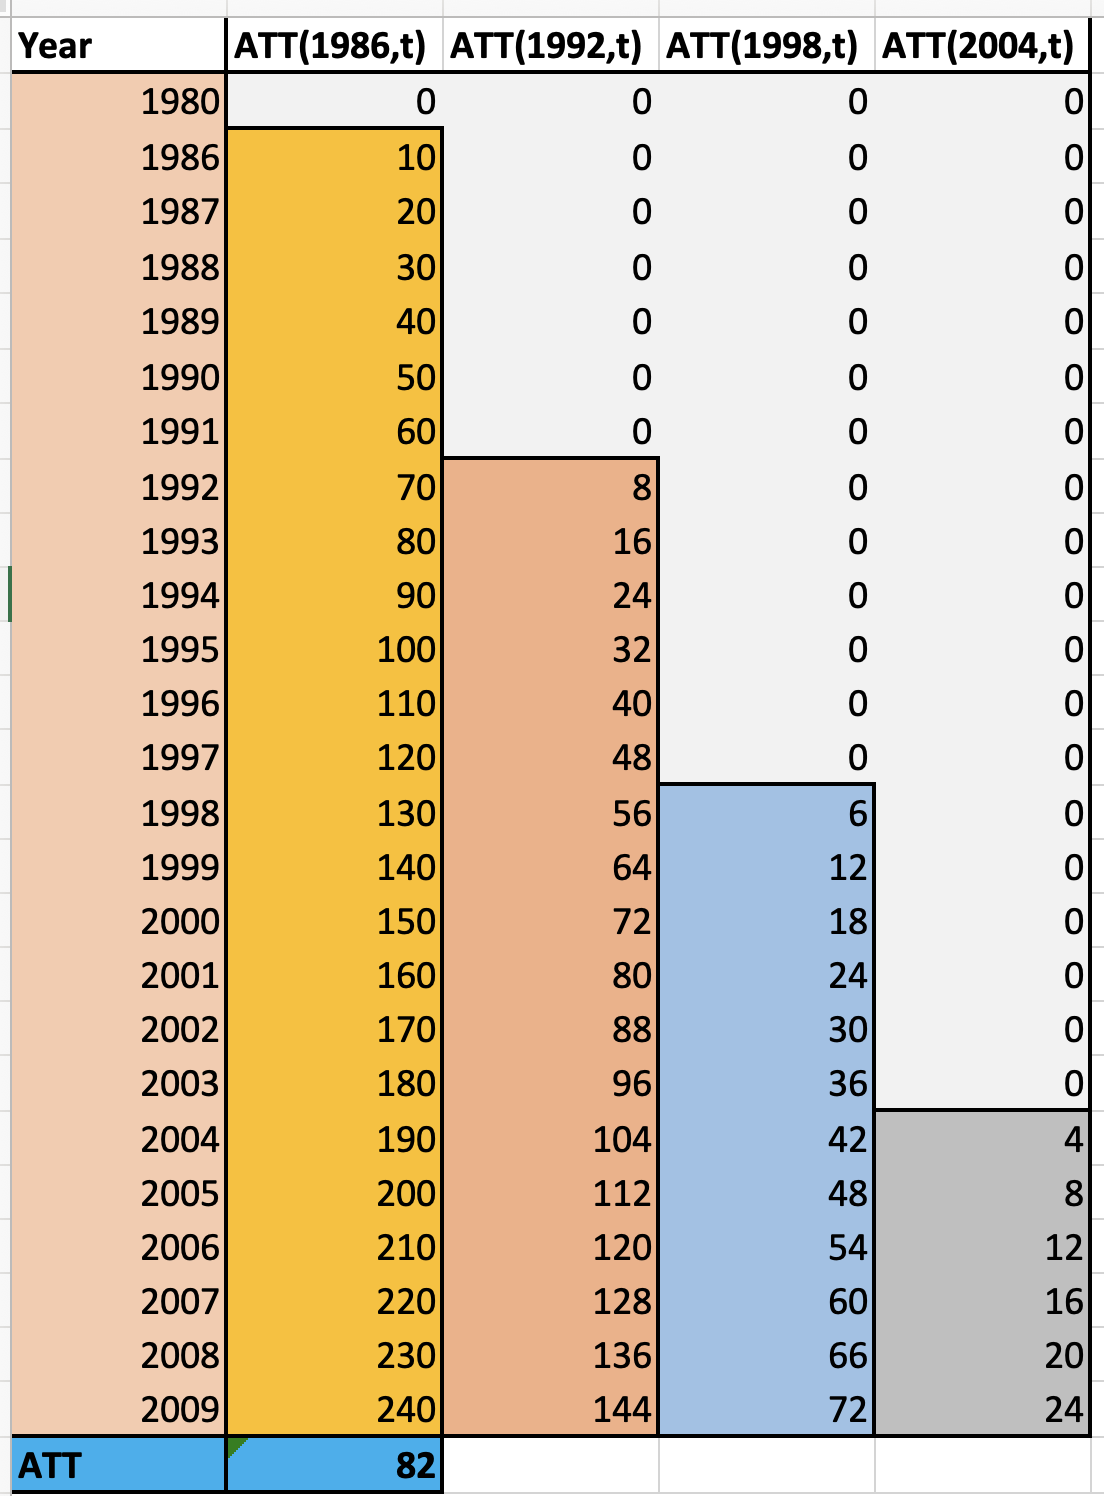
\includegraphics[height=6.5cm, width=5.5cm]{./lecture_includes/baker_attgt}
           \column{0.38\linewidth}
            Each cell contains that group's ATT(g,t)
\begin{eqnarray*}
ATT(g,t) = E[Y_t^1 - Y_t^0 | G_g=1]
\end{eqnarray*}CS identifies all feasible ATT(g,t)
         \end{columns} 
    \end{frame}




\begin{frame}{Group-time ATT}

Group-time ATT is the ATT for a specific group and time
\begin{itemize}
\item Groups are basically cohorts of units treated at the same time
\item Group-time ATT estimates are simple (weighted) differences in means
\item Does not directly restrict heterogeneity with respect to observed covariates, timing or the evolution of treatment effects over time
\item Allows us ways to choose our aggregations
\item Inference is the bootstrap or analytical standard errors based on the influence function
\end{itemize}

\end{frame}



\begin{frame}{Notation}

\begin{itemize}
\item $T$ periods going from $t=1, \dots, T$
\item Units are either treated ($D_t=1$) or untreated ($D_t=0$) but once treated cannot revert to untreated state
\item $G_g$ signifies a group and is binary.  Equals one if individual units are treated at time period $t$.
\item $C$ is also binary and indicates a control group unit equalling one if ``never treated'' (can be relaxed though to ``not yet treated'')
	\begin{itemize}
	\item Recall the problem with TWFE on using treatment units as controls
	\end{itemize}
\item Generalized propensity score enters into the estimator as a weight: $$\widehat{p(X)} = Pr(G_g=1 | X,G_g+C=1)$$
\end{itemize}

\end{frame}

\begin{frame}{Assumptions}

Assumption 1: Irreversible treatment \\
Assumption 2: Conditional parallel trends (for either never treated or not yet treated) \\
\begin{eqnarray*}
E[Y_t^0 - Y_{t-1}^0 | X,G_g=1] = [Y_t^0 - Y_{t-1}^0 | X,C=1] 
\end{eqnarray*}
\bigskip
Assumption 3: Common support (propensity score) \\
\bigskip
Assumption 4: No Anticipation

\end{frame}

\begin{frame}{CS Estimator (the IPW version)}

\begin{eqnarray*}
ATT(g,t) = E \bigg [ \bigg ( \frac{G_g}{E[G_g]} - \frac{ \frac{\hat{p}(X)C}{1-\hat{p}(X)}}{E \bigg [ \frac{\hat{p}(X)C}{1-\hat{p}(X)} \bigg ]} \bigg ) (Y_t - Y_{g-1} ) \bigg ) \bigg ]
\end{eqnarray*}

This is the inverse probability weighting estimator.  Alternatively, there is an outcome regression approach and a doubly robust. Sant'Anna recommends DR.  CS uses the never-treated or the not-yet-treated as controls but never the already-treated 
\end{frame}




\begin{frame}{Aggregated vs single year/group ATT}

\begin{itemize}
\item The method they propose is really just identifying very narrow ATT per group time.
\item But we are often interested in  more aggregate parameters, like the ATT across all groups and all times
\item They present two alternative methods for building ``interesting parameters'' 
\item Inference from a bootstrap or influence function
\end{itemize}


\end{frame}



\begin{frame}{Group-time ATT }
             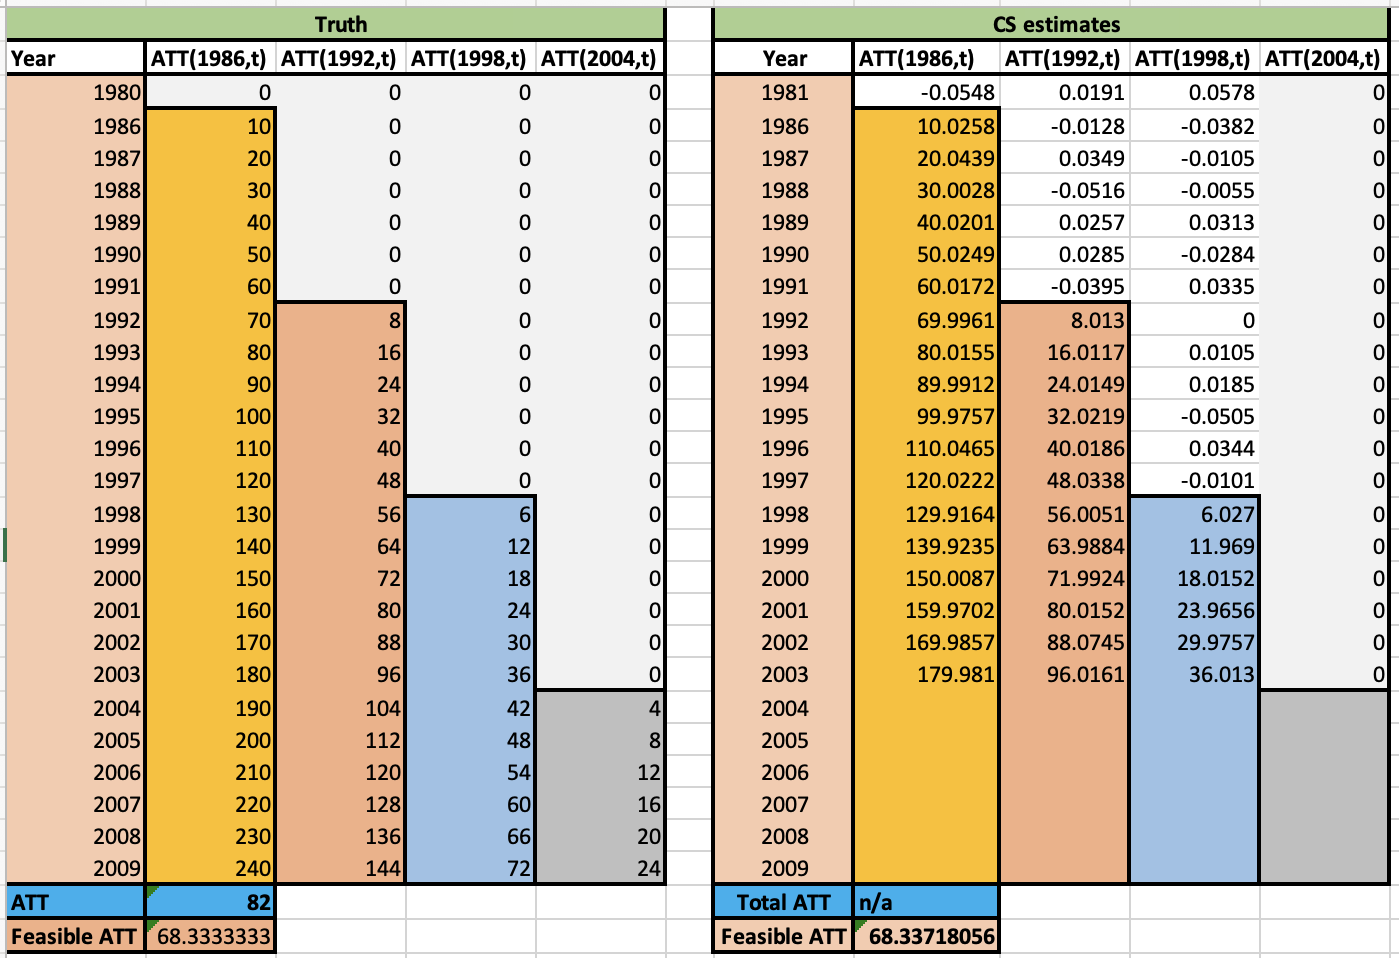
\includegraphics[scale=0.45]{./lecture_includes/baker_attgt_cs}

Question: Why didn't CS estimate all ATT(g,t)? What is ``feasible ATT''?

\end{frame}

\begin{frame}{Reporting results}
\begin{table}[htbp]\centering
\small
\caption{Estimating ATT using only pre-2004 data}
\begin{center}
\begin{tabular}{l*{5}{c}}
\hline
\multicolumn{1}{l}{\textbf{}}&
\multicolumn{1}{c}{\textbf{(Truth)}}&
\multicolumn{1}{c}{\textbf{(TWFE)}}&
\multicolumn{1}{c}{\textbf{(CS)}}&
\multicolumn{1}{c}{\textbf{(SA)}}&
\multicolumn{1}{c}{\textbf{(BJS)}}\\
\hline
$\widehat{Feasible\ ATT}$  & 68.33    & 26.81 *** & 68.34*** &&\\
\hline
\end{tabular}
\end{center}
\end{table}

TWFE is no longer negative, interestingly, once we eliminate the last group (giving us a never-treated group), but is still suffering from attenuation bias. 

\end{frame}

\subsection{Sun and Abraham (SA)}




\begin{frame}{Event study and differential timing}

\begin{itemize}
\item Sometimes we care about a simple summary, and sometimes we care about separating it out in time and sometimes in even more interesting ways
\item Event studies with one treatment group and one untreated group were relatively straightforward
\item Interact treatment group with calendar date to get a series of leads and lags
\item But when there are more than one treatment group, specification challenges emerge
\end{itemize}

\end{frame}





\begin{frame}{Bias of TWFE Event Study Specification}

\begin{itemize}
\item Bacon only focused on the static specification, and that's where the biases due to dynamics revealed itself
\item Sophie Sun and Sarah Abraham did though -- prompted by a stray comment by their professor
\item But they also unlike Bacon present a solution (which is like CS, but discovered independently)
\end{itemize}

\end{frame}

\begin{frame}{Event study specification with TWFE}


\begin{eqnarray*}
Y_{i,t} = \alpha_i + \delta_t + \sum_{g \in G} \mu_g1\{t-E_i \in g \} + \varepsilon_{i,t}
\end{eqnarray*}

\bigskip

We will focus on the coefficient $\widehat{\mu_g}$ when estimated with TWFE

\end{frame}




\begin{frame}{Sun and Abraham 2021}

	\begin{enumerate}
	\item SA shows a decomposition of the population regression coefficient on event study leads and lags with differential timing estimated with TWFE
	\item They show that the population regression coefficient is ``contaminated'' by information from other leads and lags (which is then later generalized by Goldsmith-Pinkham, Hull and Kolesar 2022)
	\item SA presents an alternative estimator that is a version of CS only using the ``last cohort'' as the comparison group (not the not-yet-treated)
	\item Derives the variance of the estimator instead of bootstrapping, handles covariates differently than CS, but otherwise identical
	\end{enumerate}

\end{frame}

\begin{frame}{Summarizing (cont.)}

\begin{itemize}
\item Under homogenous treatment profiles, weights sum to zero and ``cancel out'' the treatment effects from other periods 
\item Under treatment effect heterogeneity, they do not cancel out and leads and lags are biased
\item They present a 3-step TWFE based alternative estimator which addresses the problems that they find
\end{itemize}

\end{frame}


\begin{frame}{Some notation and terms}

\begin{itemize}
\item As people often \textbf{bin} the data, we allow a lead or lag $l$ to appear in bin $g$ so sometimes they use $g$ instead of $l$ or $l \in g$
\item Building block is the ``cohort-specific ATT'' or $CATT_{e,l}$ -- same as ATT(g,t)
\item Our goal is to estimate $CATT_{l}$ with population regression coefficient $\mu_l$
\item They focus on irreversible treatment where treatment status is non-decreasing sequence of zeroes and ones
\end{itemize}

\end{frame}



\begin{frame}{Difficult notation (cont.)}

\begin{itemize}
\item The $\infty$ symbol is used to either describe the group ($E_i=\infty$) or the potential outcome ($Y^{\infty}$)
\item $Y^{\infty}_{i,t}$ is is the potential outcome for unit $i$ if it had never received treatment (versus received it later), also called the baseline outcome
\item Other counterfactuals are possible -- maybe unit $i$ isn't ``never treated'' but treated later in counterfactual
\end{itemize}
\end{frame}

\begin{frame}{More difficult notation (cont.)}

\begin{itemize}
\item Treatment effects are the difference between the observed outcome relative to the never-treated counterfactual outcome: $Y_{i,t} - Y^{\infty}_{i,t}$
\item We can take the average of treatment effects at a given relative time period across units first treated at time $E_i=e$ (same cohort) which is what we mean by $CATT_{e,l}$
\item Doesn't use $t$ index time (``calendar time''), rather uses $l$ which is time until or time after treatment date $e$ (``relative time'')
\item Think of it as ${l}=$year - treatment date
\end{itemize}

\end{frame}

\begin{frame}{Relative vs calendar event time}


\begin{figure}
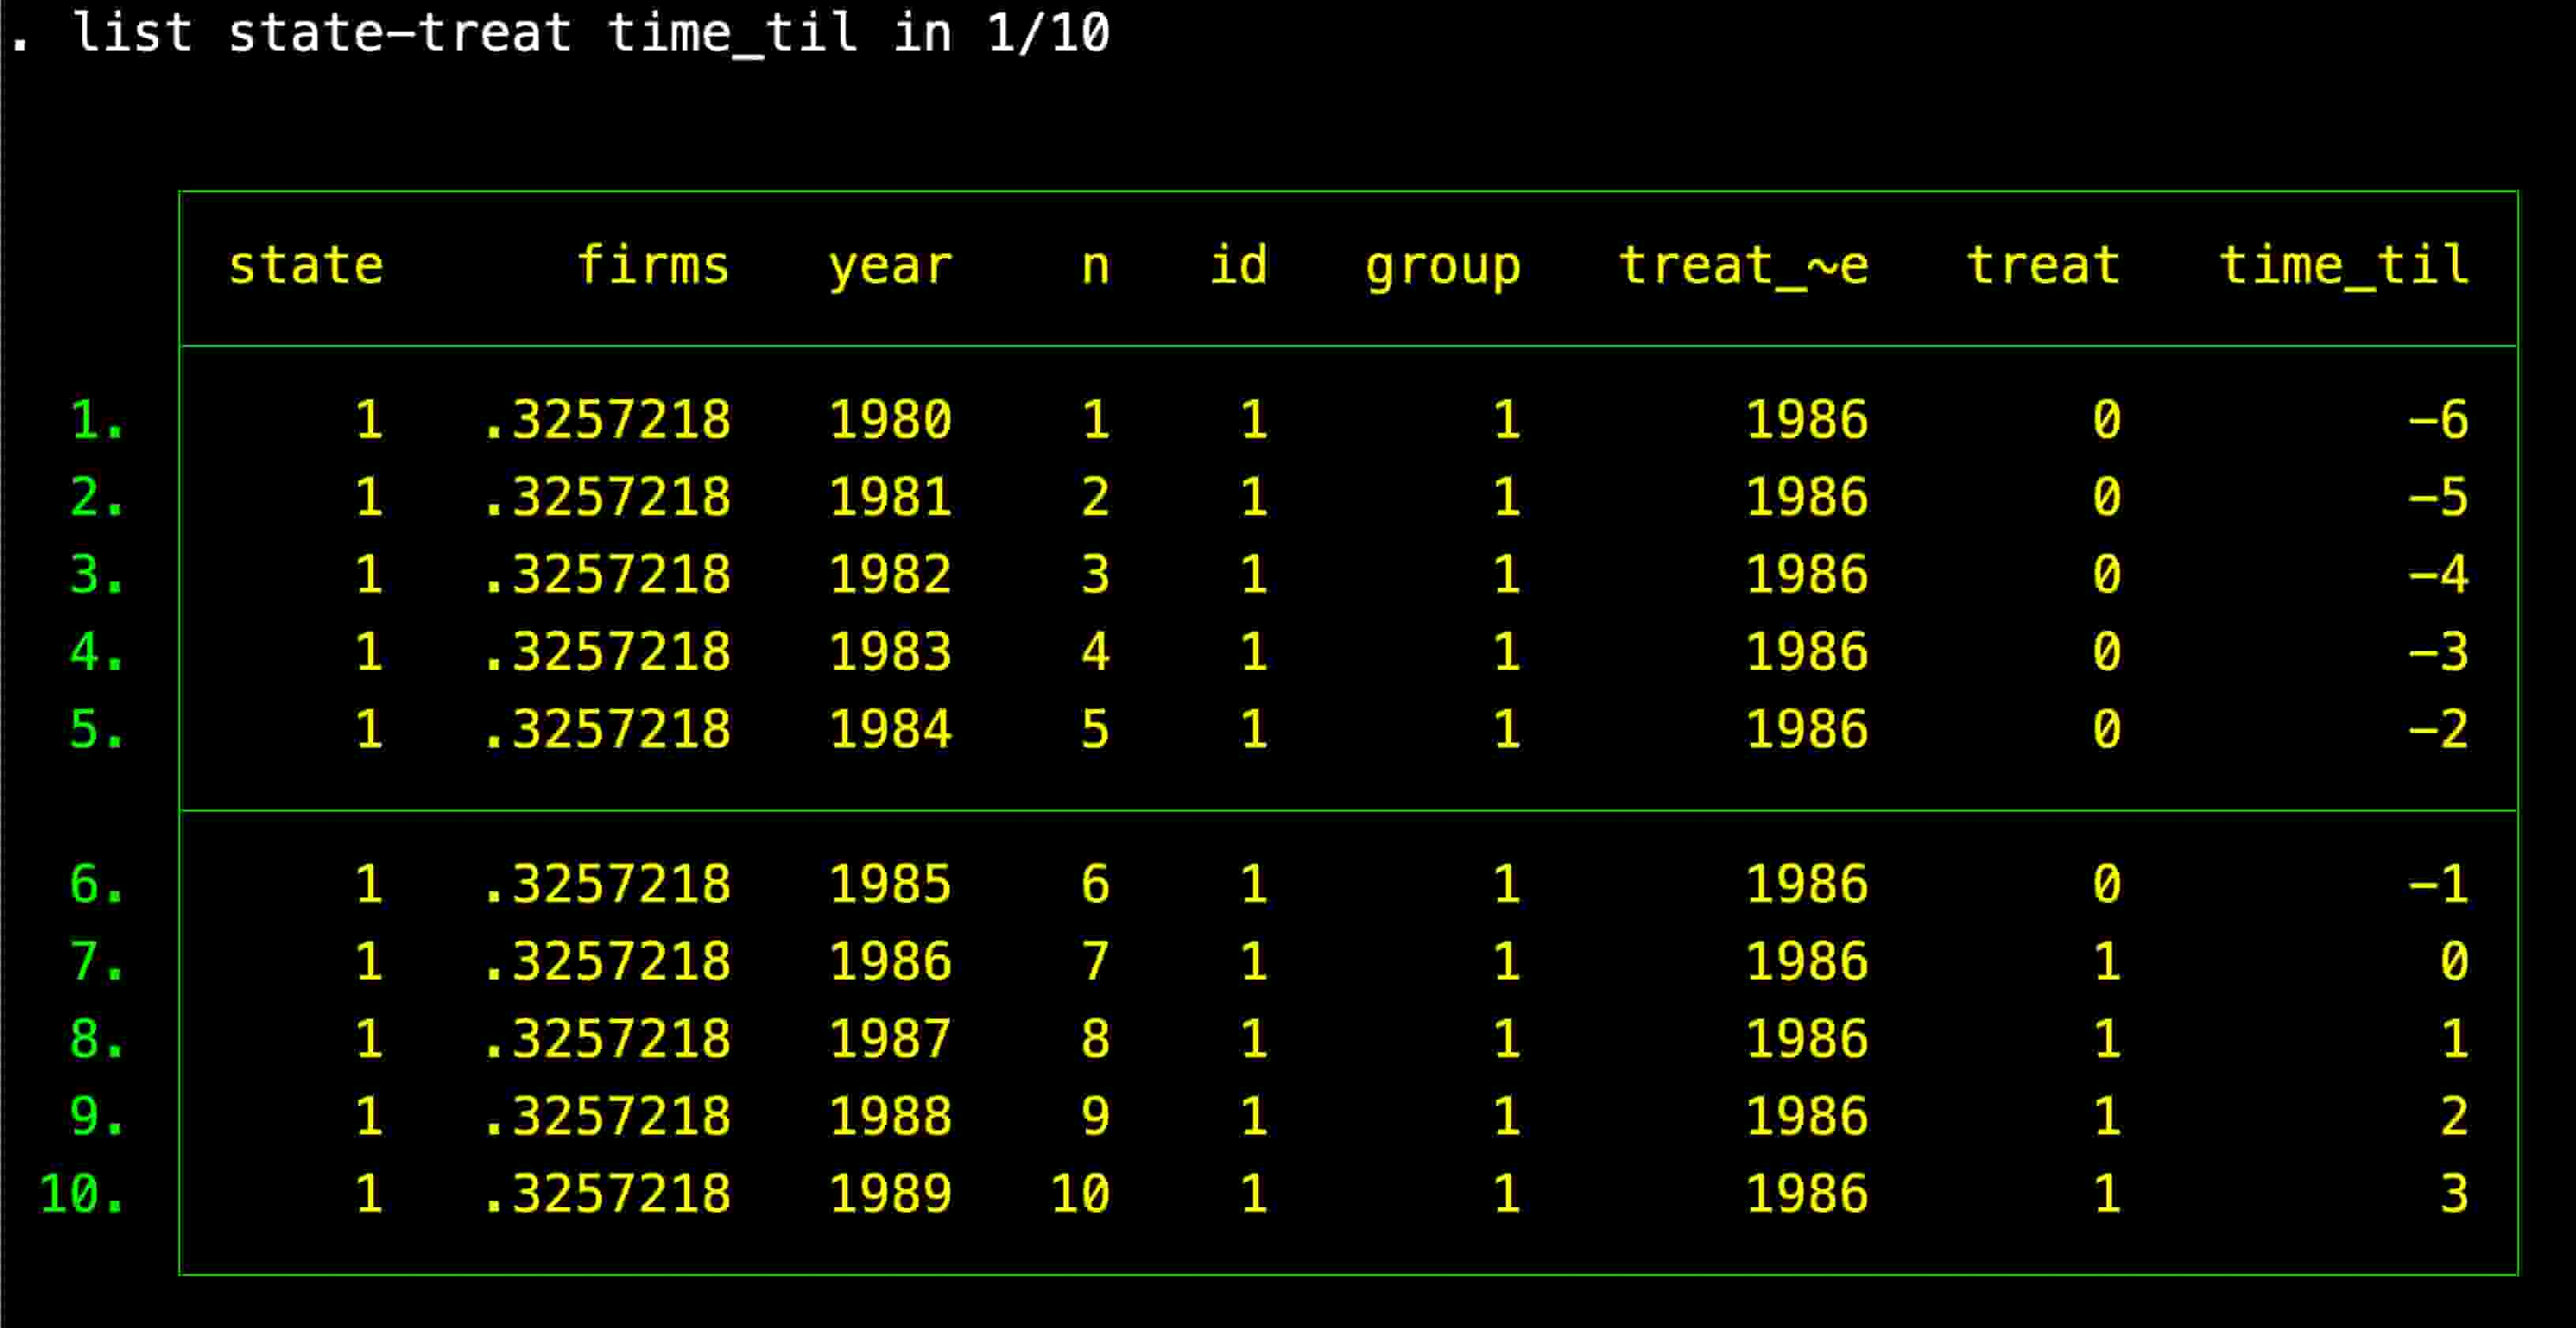
\includegraphics[scale=0.2]{./lecture_includes/timetil}
\end{figure}

\end{frame}


\begin{frame}{Definition 1}

\textbf{Definition 1:} The cohort-specific ATT $l$ periods from initial treatment date $e$ is:

\begin{eqnarray*}
CATT_{e,l} = E[Y_{i,e+l} - Y^{\infty}_{i,e+l} | E_i=e]
\end{eqnarray*}

\bigskip

Fill out the second part of the Group-time ATT exercise together.

\end{frame}

\begin{frame}{TWFE assumptions}

\begin{itemize}
\item For consistent estimates of the coefficient leads and lags using TWFE model, we need three assumptions
\item For SA and CS, we only need two
\item Let's look then at the three
\end{itemize}

\end{frame}


\begin{frame}{Assumption 1: Parallel trends}

\textbf{Assumption 1: Parallel trends in baseline outcomes}: $E[Y^{\infty}_{i,t} - Y^{\infty}_{i,s} | E_i = e ]$ is the same for all $e \in supp(E_i)$ and for all $s$, $t$ and is equal to $E[Y^{\infty}_{i,t} - Y^{\infty}_{i,s} ]$

\bigskip

Lead and lag coefficients are DiD equations but once we invoke parallel trends they can become causal parameters.  This reminds us again how crucial it is to have  appropriate controls

\end{frame}


\begin{frame}{Assumption 2: No anticipation}

\textbf{Assumption 2: No anticipator behavior in pre-treatment periods}: There is a set of pre-treatment periods such that $E[Y_{i,e+l}^e - Y_{i,e+l}^{\infty} | E_i = e]=0$ for all possible leads.

\bigskip

Essentially means that pre-treatment, the causal effect is zero.  Most plausible if no one sees the treatment coming, but even if they see it coming, they may not be able to make adjustments that affect outcomes

\end{frame}


\begin{frame}{Assumption 3: Homogeneity}

\textbf{Assumption 3: Treatment effect profile homogeneity}: For each relative time period $l$, the $CATT_{e,l}$ doesn't depend on the cohort and is equal to $CATT_l$. 


\end{frame}

\begin{frame}{Treatment effect heterogeneity}

\begin{itemize}
\item Assumption 3 is violated when different cohorts experience different paths of treatment effects
\item Cohorts may differ in their covariates which affect how they respond to treatment (e.g., if treatment effects vary with age, and there is variation in age across units first treated at different times, then there will be heterogeneous treatment effects)
\item Doesn't rule out parallel trends
\end{itemize}

\end{frame}

\begin{frame}{Event study model}

Dynamic TWFE model

\begin{eqnarray*}
Y_{i,t} = \alpha_i + \delta_t + \sum_{g \in G} \mu_g1\{t-E_i \in g \} + \varepsilon_{i,t}
\end{eqnarray*}

\bigskip

We are interested in the properties of $\mu_g$ under differential timing as well as whether there are any never-treated units

\end{frame}



\begin{frame}[plain, shrink=20]
\begin{center}
\textbf{Interpreting $\widehat{\mu_g}$ under no to all assumptions}
\end{center}

\textbf{Proposition 1 (no assumptions):} The population regression coefficient on relative period bin $g$ is a linear combination of differences in trends from its own relative period $l \in g$, from relative periods $l \in g'$ of other bins $g' \neq g$, and from relative periods excluded from the specification (e.g., trimming). 

\begin{eqnarray*}
\mu_g &=& \underbrace{\sum_{l \in g} \sum_{e} w^g_{e,l} \big ( E[Y_{i,e+l} - Y^{\infty}_{i,0} | E_i = e] - E[Y^{\infty}_{i,e+l} - Y^{\infty}_{i,0}] \big )}_{\mathclap{\text{Targets}}} \\
&+& \underbrace{\sum_{g' \neq g} \sum_{l \in g'} \sum_e w^g_{e,l} \big ( E[Y_{i,e+l} - Y^{\infty}_{i,0} | E_i=e] - E[Y^{\infty}_{i,e+l} - Y^{\infty}_{i,0}] \big )}_{\mathclap{\text{Contamination from other leads and lags}}} \\
&+&  \underbrace{\sum_{l \in g^{excl}} \sum_{e} w^g_{e,l} \big ( E[Y_{i,e+l} - Y^{\infty}_{i,0} | E_i=e] - E[Y^{\infty}_{i,e+l} - Y^{\infty}_{i,0}] \big )}_{\mathclap{\text{Contamination from dropped periods}}} 
\end{eqnarray*}

\bigskip


\end{frame}

\begin{frame}{Weight ($w^g_{e,l}$) summation cheat sheet}

\begin{enumerate}
\item For relative periods of $\mu_g$ own $l \in g$, $\sum_{l \in g}\sum_ew^g_{e,l}=1$
\item For relative periods belonging to some other bin $l\in g'$ and $g' \neq g$, t $\sum_{l \in g'}\sum_ew^g_{e,l} = 0$
\item For relative periods not included in $G$, $\sum_{l \in g^{excl}} \sum_e w^g_{e,l} = -1$
\end{enumerate}

\end{frame}




\begin{frame}{Estimating the weights}

Regress $D^l_{i,t} \times 1\{E_i=e \}$ on:

\begin{enumerate}
\item all bin indicators included in the main TWFE regression, 
\item $\{ 1\{ t-E_i \in g \} \}_{g \in G}$(i.e., leads and lags) and 
\item the unit and time fixed effects
\end{enumerate}

\end{frame}


\begin{frame}{Still biased under parallel trends}

\textbf{Proposition 2}: Under the parallel trends only, the population regression coefficient on the indicator for relative period bing $g$ is a linear combination of $CATT_{e,l \in g}$ as well as $CATT_{d,l'}$ from other relative periods $l' \notin g$ with the same weights stated in Proposition 1:

\begin{eqnarray*}
\mu_g &=& \underbrace{\sum_{l \in g} \sum_e w^g_{e,l} CATT_{e,l}}_{\mathclap{\text{Desirable}}} \\
&& + \underbrace{\sum_{g' \neq g, g' \in G} \sum_{l' \in g'} \sum_e w^g_{e,l'}  CATT_{e,l'}}_{\mathclap{\text{Bias from other specified bins}}} \\
&&+ \underbrace{\sum_{l' \in g^{excl}} \sum_e w^g_{e,l'} CATT_{e,l'}}_{\mathclap{\text{Bias from dropped relative time indicators}}}
\end{eqnarray*}



\end{frame}


\begin{frame}{Still biased under parallel trends and no anticipation}

\textbf{Proposition 3}: If parallel trends holds and no anticipation holds for all $l<0$ (i.e., no anticipatory behavior pre-treatment), then the population regression coefficient $\mu_g$ for $g$ is a linear combination of post-treatment $CATT_{e,l'}$ for all $l' \geq 0$.

\begin{eqnarray*}
\mu_g &=& \sum_{l' \in g, l' \geq 0} \sum_e w^g_{e,l'} CATT_{e,l'} \\
&&+ \sum_{g' \neq g,g' \in G} \sum_{l' \in g', l' \geq 0} \sum_e w^g_{e,l'} CATT_{e,l'} \\
&&+ \sum_{l' \in g^{excl},l' \geq 0} \sum_e w^g_{w,l'} CATT_{e,l'}
\end{eqnarray*}

\end{frame}

\begin{frame}{Proposition 3 comment}

Notice how once we impose zero pre-treatment treatment effects, those terms are gone (i.e., no $l \in g, l<0$).  But the second term remains unless we impose treatment effect homogeneity (homogeneity causes terms due to weights summing to zero to cancel out). Thus $\mu_g$ may be non-zero for pre-treatment periods \emph{even though parallel trends hold in the pre period.}

\end{frame}

\begin{frame}{Proposition 4}

\textbf{Proposition 4}: If parallel trends and treatment effect homogeneity, then $CATT_{e,l}=ATT_l$ is constant across $e$ for a given $l$, and the population regression coefficient $\mu_g$ is equal to a linear combination of $ATT_{l \in g}$, as well as $ATT_{l' \notin g}$ from other relative periods

\begin{eqnarray*}
\mu_g &=& \sum_{l \in g} w^g_l ATT_l \\
&&+ \sum_{g' \neq g} \sum_{l' \in g'} w^g_{l'} ATT_{l'} \\
&&+ \sum_{l' \in g^{excl}} w^g_{l'}ATT_{l'}
\end{eqnarray*}


\end{frame}

\begin{frame}{Simple example}


Balanced panel $T=2$ with cohorts $E_i \in \{1,2 \}$. For illustrative purposes, we will include bins $\{-2,0\}$ in our calculations but drop $\{-1,1\}$. 


\end{frame}

\begin{frame}{Simple example}

\begin{eqnarray*}
\mu_{-2} &=& \underbrace{CATT_{2,-2}}_{\mathclap{\text{own period}}} + \underbrace{\frac{1}{2}CATT_{1,0} - \frac{1}{2} CATT_{2,0}}_{\mathclap{\text{other included bins}}} \\
&&+ \underbrace{ \frac{1}{2} CATT_{1,1} - CATT_{1,-1} - \frac{1}{2} CATT_{2,-1} }_{\mathclap{\text{Excluded bins}}}
\end{eqnarray*}

\begin{itemize}
\item Parallel trends gets us to all of the $CATT$
\item No anticipation makes $CATT=0$ for all $l<0$ (all $l<0$ cancel out)
\item Homogeneity cancels second and third terms
\item Still leaves $\frac{1}{2} CATT_{1,1}$ -- you chose  to exclude a group with a treatment effect
\end{itemize}Lesson: drop the relative time indicators on the left, not things on the right, bc lagged effects will contaminate through the excluded bins


\end{frame}


\begin{frame}{Robust event study estimation}


\begin{itemize}
\item All the robust estimators under differential timing have solutions and they all skip over forbidden contrasts. 
\item Sun and Abraham (2021) propose a 3-step interacted weighted estimator (IW) using last treated group as control group
\item Callaway and Sant'anna (2021) estimate group-time ATT which can be a weighted average over relative time periods too but uses ``not-yet-treated'' as control
\end{itemize}

\end{frame}




\begin{frame}{Interaction-weighted estimator}

\begin{itemize}
\item \textbf{Step one}: Do this DD regression and hold on to $\widehat{\delta}_{e,l}$
\end{itemize}

\begin{eqnarray*}
Y_{i,t} = \alpha_i + \lambda_t + \sum_{e \notin C} \sum_{l \neq -1} \delta_{e,l} \big (1 \{ E_i = e \} \cdot D_{i,t}^l \big ) + \varepsilon_{i,t}
\end{eqnarray*}


\bigskip

Can use never-treated or last-treated cohort. Drop always treated. The $\delta_{e,l}$ is a DD estimator for $CATT_{e,l}$ with particular choices for pre-period and cohort controls

\end{frame}


\begin{frame}{Interaction-weighted estimator}

\begin{itemize}
\item \textbf{Step two}: Estimate weights using sample shares of each cohort in the relevant periods:
\end{itemize}

\begin{eqnarray*}
Pr(E_i=e|E_i \in [-l,T-l])
\end{eqnarray*}

\end{frame}

\begin{frame}{Interaction-weighted estimator}

\begin{itemize}
\item \textbf{Step three}: Take a weighted average of estimates for $CATT_{e,l}$ from Step 1 with weight estimates from step 2
\end{itemize}


\begin{eqnarray*}
\widehat{v}_g = \frac{1}{|g|} \sum_{l \in g} \sum_e \widehat{\delta}_{e,l} \widehat{Pr} \{ E_i=e | E_i \in [-l,T-l]\}
\end{eqnarray*}


\end{frame}

\begin{frame}{Consistency and Inference}


\begin{itemize}
\item Under parallel trends and no anticipation, $\widehat{\delta}_{e,l}$ is consistent, and sample shares are also consistent estimators for population shares. 
\item Thus IW estimator is consistent for a weighted average of $CATT_{e,l}$ with weights equal to the share of each cohort in the relevant period(s).
\item They show that each IW estimator is asymptotically normal and derive its asymptotic variance. Doesn't rely on bootstrap like CS.
\end{itemize}

\end{frame}

\begin{frame}{DD Estimator of CATT}

\textbf{Definition 2}: DD estimator with pre-period $s$ and control cohorts $C$ estimates $CATT_{e,l}$ as:

\begin{eqnarray*}
\widehat{\delta_{e,l}} = \frac{ E_N \big [ \big ( Y_{i, e+l} - Y_{i,s} \big ) \times 1\{E_i=e\} \big ]}{E_N[1 \{E_i=e\} ]} - \frac{E_N \big [ \big ( Y_{i,e+l} \times 1 \{E_i \in C \} ]}{E_N [1 \{ E_i \in C \}]}
\end{eqnarray*}


\textbf{Proposition 5}: If parallel trends and no anticipation both hold for all pre-periods, then the DD estimator using any pre-period and non-empty control cohorts (never-treated or not-yet-treated) is an unbiased estimate for $CATT_{e,l}$

\end{frame}

\begin{frame}{Software}

\begin{itemize}
\item \textbf{Stata}: eventstudyinteract (can be installed from ssc)
\item \textbf{R}: fixest with subab() option (see \url{https://lrberge.github.io/fixest/reference/sunab.html/})
\end{itemize}


\end{frame}


\begin{frame}{Reporting results}
\begin{table}[htbp]\centering
\small
\caption{Estimating ATT}
\begin{center}
\begin{tabular}{l*{5}{c}}
\hline
\multicolumn{1}{l}{\textbf{}}&
\multicolumn{1}{c}{\textbf{(Truth)}}&
\multicolumn{1}{c}{\textbf{(TWFE)}}&
\multicolumn{1}{c}{\textbf{(CS)}}&
\multicolumn{1}{c}{\textbf{(SA)}}&
\multicolumn{1}{c}{\textbf{(BJS)}}\\
\hline
$\widehat{Feasible\ ATT}$  & 68.33    & 26.81*** & 68.34*** & 68.33***&\\
\hline
\end{tabular}
\end{center}
\end{table}

\end{frame}

\begin{frame}{Computing relative event time leads and lags }
             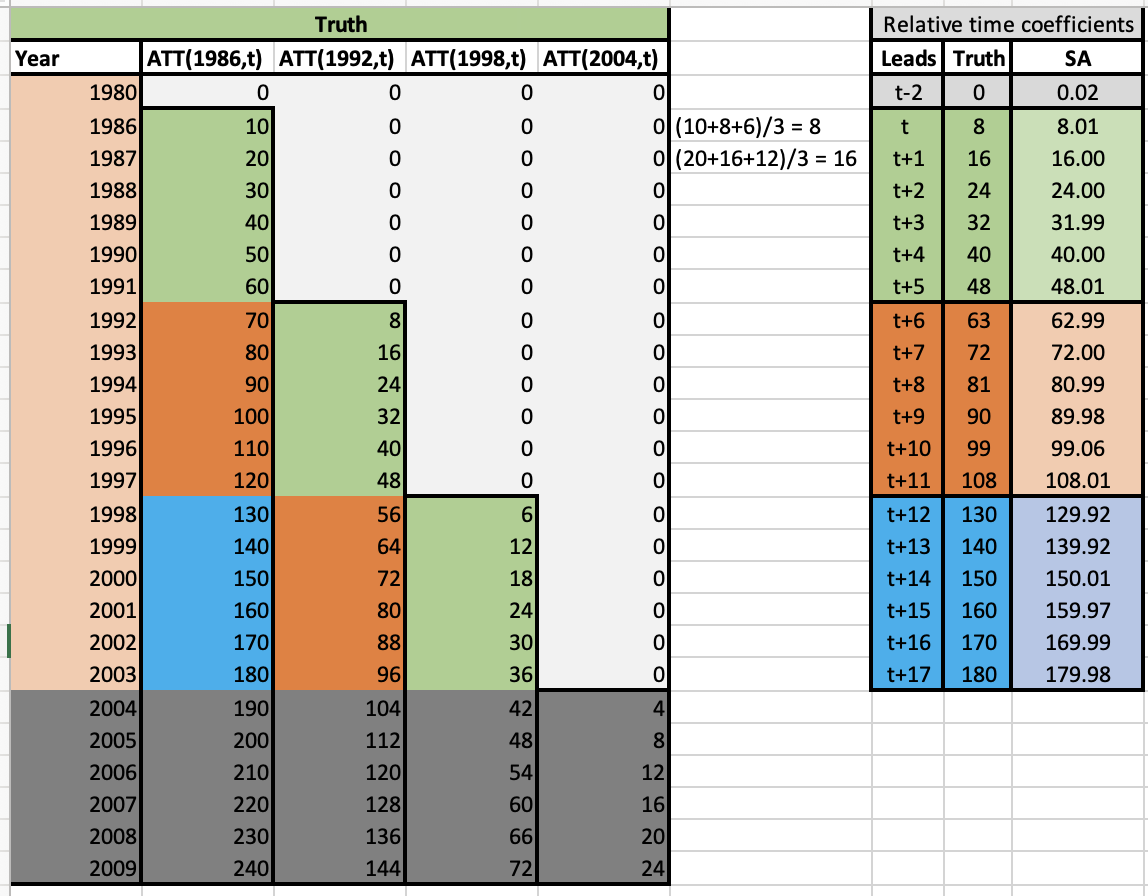
\includegraphics[scale=0.45]{./lecture_includes/sa_leads}

Two things to notice: (1) there only 17 lags with robust models but will be 24 with TWFE; (2) changing colors mean what?

\end{frame}

\begin{frame}{Comparing TWFE and SA }

\begin{figure}
\begin{center}
             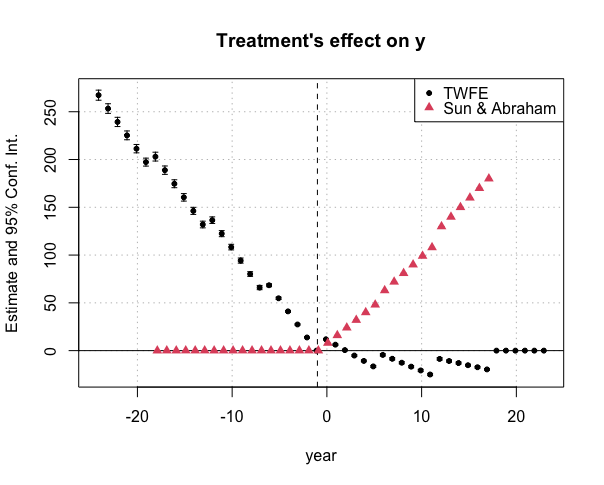
\includegraphics[scale=0.4]{./lecture_includes/twfe_sa_event}
\end{center}
\end{figure}

Question: why is TWFE \emph{falling} pre-treatment?  Why is SA rising, but jagged, post-treatment?

\end{frame}


\subsection{de Chaisemartin and D'Haultfoeulle (dCDH)}

\begin{frame}{de Chaisemartin and D'Haultfoeulle 2020}

de Chaisemartin and D'Haultfouelle 2020 (dCDH) is different from the other papers in several ways
	\begin{itemize}
	\item Like SA, it's reverse engineering and forward engineering
	\item TWFE decomposition shows coefficient a weighted average of underlying treatment effects, but weights can be negative negating causal interpretation
	\item Propose a solution for both static and dynamic specification which does not use already treated as controls
	\item Treatment can turn on and off
	\end{itemize}

\end{frame}


\begin{frame}{Comment on Bacon}

\begin{itemize}
\item Recall the Bacon decomposition -- TWFE coefficients are decomposed into weighted average of all underlying 2x2s. Weights were non-negative and summed to one.
\item But this decomposition was more a numerical decomposition -- what exactly adds up to equal the TWFE coefficient using the data we observe?
\item Bacon's decomposition is not ``theoretical'' -- not in the way that other decompositions are. He is just explaining what OLS ``does'' when it calculates $\widehat{\delta}$
\item Just explains what comparisons OLS is using to calculate the TWFE coefficient -- just peels back the curtain.
\end{itemize}

\end{frame}

\begin{frame}{Negative weights}

\begin{itemize}
\item dCDH impose causal assumptions and try a different decomposition strategy
\item Uses as its building block the unit-specific treatment effects
\item Their decomposition will reveal negative weights on the underlying treatment effects (similar to negative weight on dynamics with Bacon)
\item Remember though: the Bacon decomposition weights were \emph{always} positive, because they were numerical weights (not theoretical weights) on the underlying 2x2s (not the treatment effects)
\end{itemize}

\end{frame}

\begin{frame}{Turning on and off}

\begin{itemize}
\item CS and SA both require interventions to turn on and stay on
\item dCDH allows for ``switching'' on and off (but assumptions and control group needed might surprise you)
\item Before we move quickly into that, please note that the researcher bears the burden of knowing whether in fact you want to impose symmetry on turning on and off
\item Roe v Wade ``turned on'' legalized abortion and 2022 it was ``turned off'' -- do we want to treat these as simply a single policy flipping of the switch or two separate policies?
\end{itemize}

\end{frame}

\begin{frame}{dCDH notation}

\begin{itemize}
\item Individual treatment effects (iow, not the group-time ATT): $$\Delta^g_{i,t} = Y^1_{i,t} - Y^\infty_{i,t}$$ but where the treatment is in time period $g$. Notice --it's not the ATT (it's $i$ individual treatment effect)
\item with defined error term as $\varepsilon_{i,t}$: $$D_{i,t} = \alpha_i + \alpha_t + \varepsilon_{i,t}$$
\item Weights: $$w_{i,t} = \frac{\varepsilon_{i,t}}{\frac{1}{N^T} \sum_{i,t:D_{i,t}=1} \varepsilon_{i,t}}$$
\end{itemize}

\end{frame}

\begin{frame}{Parallel trend assumption}

\begin{block}{Strong unconditional PT}
Assume that for every time period $t$ and every group $g,g'$, $$E[Y^\infty_t - Y^\infty_{t-1}|G=g] = E[Y^\infty_t - Y^\infty_{t-1}|G=g'] $$
\end{block}Assume parallel trends for every unit in every cohort in every time period.

\bigskip

What then does TWFE estimate with differential timing?

\end{frame}

\begin{frame}{dCDH Theorem}

\begin{block}{Theorem -- dCDH decomposition}
Assuming SUTVA, no anticipation and the strong PT, then let $\delta$ be the TWFE estimand associated with $$Y_{i,t} = \alpha_i + \alpha_t + \delta D_{i,t} + \varepsilon_{i,t}$$Then it follows that $$\delta = E \bigg [ \sum_{i,t:D_{i,t}=1} \frac{1}{N^T} w_{i,t} \cdot \Delta_{i,t}^g \bigg ] $$ where $\sum_{i,t:D_{i,t}=1} \frac{w_{i,t}}{N^T} = 1$ but $w_{i,t}$ can be negative
\end{block}

\end{frame}

\begin{frame}{Origins}

\begin{itemize}
\item So once you run that specification, $\widehat{\delta}$ is going to recover a ``non-convex average'' over all unit level treatment effects (weights can be negative, more on this). 
\item Very important theorem -- established the ``no sign flip property'' for OLS with differential timing in the canonical static specification
\end{itemize}

\end{frame}





\begin{frame}{OLS Weighting}

\begin{itemize}
\item The economic question is ``what parameter do you want? What does it look like? Who is in it?''
\item And when you define the parameter up front, you've more or less defined the economic question you're asking
\item But OLS sort of ignores your question and just gives you what it wants
\item The weights in OLS all come out of the model itself, \emph{not the economic question}
\end{itemize}

\end{frame}

\begin{frame}{OLS Weighting}

\begin{itemize}
\item What makes something a good vs a bad weight?
\item Not being negative is the absolute minimal requirement
\item But that's the minimum -- we mainly are trying to weight to the target parameter, not justify the use of a model
\item It is also not a good sign if you can't really explain the weights
\end{itemize}

\end{frame}

\begin{frame}{dCdH Solution}

\begin{itemize}
\item dCdH propose an alternative that doesn't have the problems of TWFE -- both avoiding negative weights and improving interpretability
\item Their model can handle reversible treatments, but in the context of differential timing is equivalent to CS and SA with a particular choice of weights
\item For diagnostic purposes, they recommend reporting the number/fraction of group-time ATTs that receive negative weights, as well as the degree of heterogeneity in treatment effects that would be necessary for the estimated treatment effect to have the “wrong sign"

\end{itemize}

\end{frame}



\begin{frame}{DID\textsubscript{M} Estimator -- Introduction}
\begin{itemize}
\item DID\textsubscript{M} estimator from dCDH (de Chaisemartin and D'Haultfoeulle, 2020) estimates treatment effects around each treatment transition.
\item Separately captures effects for:
\begin{itemize}
    \item "Joiners" (entering treatment)
    \item "Leavers" (exiting treatment)
\end{itemize}
\item Defined as weighted average:
\[
DID_M = \text{weighted average of DID}_{+,t} \text{ and DID}_{-,t}
\]
\item Avoids TWFE negative weighting problem.
\end{itemize}
\end{frame}

\begin{frame}{Estimating DID\textsubscript{+,t} ("Turning On")}
\begin{itemize}
\item For units that begin treatment at time \( t \):
\[
DID_{+,t} = \underbrace{(Y_{t}^{newly\ treated} - Y_{t-1}^{newly\ treated})}_{\text{Change for joiners}} - \underbrace{(Y_{t}^{untreated} - Y_{t-1}^{untreated})}_{\text{Change for untreated}}
\]
\item Compares outcomes of "joiners" to those never treated.
\item Similar conceptually to Callaway \& Sant'Anna and Sun \& Abraham in scenarios where treatment turns on.
\end{itemize}
\end{frame}

\begin{frame}{Estimating DID\textsubscript{-,t} ("Turning Off")}
\begin{itemize}
  \item For units exiting treatment at time \( t \), their estimator identifies the effect of "stopping treatment"
  \begin{equation*}
    \small
    \text{DID}_{-,t} = 
    \underbrace{(Y_{t}^{\text{leavers}} - Y_{t-1}^{\text{leavers}})}_{\text{Change for leavers}} 
    - 
    \underbrace{(Y_{t}^{\text{continuously treated}} - Y_{t-1}^{\text{continuously treated}})}_{\text{Change for continuously treated}}
  \end{equation*}
  \item You are now missing $Y^1$ in this new causal effect, so you need a control group whose outcome is treated ($Y^1$)
  \item Whatever treatment state the "exiting group" had been at in baseline, the control group must be too (well defined treatment statuses again)
\end{itemize}
\end{frame}



\begin{frame}{Combining DID\textsubscript{+,t} and DID\textsubscript{-,t}}
\begin{itemize}
\item DID\textsubscript{M} combines these into a single estimate:
\[
DID_M = \sum_t \left(\text{weights}_t \cdot DID_{+,t}\right) + \sum_t \left(\text{weights}_t \cdot DID_{-,t}\right)
\]
\item Weights typically based on group size or variance.
\item Simplifies to weighted average of DID\textsubscript{+,t} when no units revert (staggered adoption without exit).
\end{itemize}
\end{frame}

\begin{frame}{Key Assumption: No Carryover}
\begin{itemize}
\item Important assumption: treatment effects disappear immediately after treatment stops (not treated if not treated)
\item If treatment effects linger, estimator will underestimate the true effect of exiting treatment.
\item Practical consideration: Is turning off treatment truly reverting to baseline, or is it moving into a different treatment state?
\end{itemize}
\end{frame}

\begin{frame}{Control Group Must Be Treated Continuously}
\begin{itemize}
\item When treatment is "switching off" (i.e., $D_i=1$ to $D_i=0$), you're going to need as your control group "always treated units"
\item This is again because when treatment is turned off, the unit has gone from $Y=Y^1$ at the new baseline to $Y=Y^0$
\item Means that for any treatment effect, the missing potential outcome will be $Y^1$, and so you'll need at both periods units "always treated" 
\item Needs parallel trends in $Y^1$ therefore -- which means they cannot be "the first to leave treatment" 
\end{itemize}
\end{frame}


\begin{frame}{Comparison to Callaway \& Sant'Anna and Sun \& Abraham}
\begin{itemize}
\item CS and SA primarily handle switching on, but switching off
\item DID\textsubscript{M} extends naturally to reversible treatments (on and off transitions)
\item But you have to be sure that parallel trends holds for the comparison group (who is continuously treated) -- again, you're not using all the data
\item All three methods avoid negative weighting problems inherent in traditional TWFE.
\end{itemize}
\end{frame}



\section{Calculating event study coefficients with new estimators}


\begin{frame}{What did regressions do?}

\begin{itemize}

\item In regressions, when you estimate leads and lags, you would drop one year dummy variable
\item By dropping one year dummy variable, all coefficients were "long difference" calculations relative to that baseline -- both the $ATT(g,t)$ but also the event study pre-treatment coefficients
\item Which means every event study plot you've ever seen with TWFE always was interpreted relative to a universal baseline (usually $t-1$)
\item Some of the new estimators will allow for a different calculation, and this has created inconsistent estimators across new papers, which are relevant for checking for pre-trends

\end{itemize}

\end{frame}




\begin{frame}{Event study lead calculation}

\begin{itemize}

\item In CS and dCDH, there are two ways to calculate the pre-treatment coefficients once you have obtained the ATT(g,t) parameter estimates:
	\begin{enumerate}
	\item \textbf{Long difference}. Uses a "universal baseline" with a fixed baseline at \( t-1 \).
	
	\begin{eqnarray*}
	 \widehat{\delta}_{t-3} = \left( E[Y|D=1, t-3] - E[Y|D=1, t-1] \right) \\
	 - \left( E[Y|D=0, t-3] - E[Y|D=0, t-1] \right)
	 \end{eqnarray*}


	\item \textbf{Short gap}. Uses a "rolling" method in which a new baseline is used for each 2x2 comparison.
	
	\begin{eqnarray*}
	 \widehat{\delta}_{t-3} = \left( E[Y|D=1, t-3] - E[Y|D=1, t-2] \right) \\
	 - \left( E[Y|D=0, t-3] - E[Y|D=0, t-2] \right)
	 \end{eqnarray*}
	 
	 \end{enumerate}
	 
 \item Both are diff-in-diff $2 \times 2$, but pre-trends can be zero in one, but not the other
	 
\end{itemize}

\end{frame}





\begin{frame}{What is the event study for?}

\begin{itemize}

\item The purpose of the event study is as a \emph{falsification}, not as a proof of the parallel trends
\item Falsifications should be the \emph{same} model used for estimation but applied to something that it cannot cause -- "same group, different outcome"
\item In this case, future treatments under no anticipation cannot affect the past
\item Since the estimation of post-treatment ATT use $t-1$ for "pre" period, the falsifications in the event studies should too 
\end{itemize}

\end{frame}


\begin{frame}{Detecting it in papers}

\begin{itemize}

\item Very easy to spot which method someone used 
\item Long differences \emph{never} have a coefficient at baseline, because long differences uses baseline as the comparison \emph{always}
\item Short gaps will \emph{always} have a coefficient at baseline

\end{itemize}

\end{frame}

\begin{frame}{Detecting it in papers}

\begin{itemize}

\item Interestingly, long differences and short gaps have the same information -- you can easily convert one into the other -- but one will show trends and the other won't
\item So which one is right?  Remember -- parallel trends is a long difference, and all calculations are long differences, even in CS, so in my opinion so should the event study coefficients
\item Plus remember -- TWFE invented the event study, long differences is what we expect, so it's a subtle switching out of visualizing pre-trends from our expectation
\item Let's look at a simulation by Jon Roth (2024) where he build data with rising pre-trends which he then estimated with TWFE (long difference), CS (short gaps), dCDH (short gaps) and BJS (Kyle can discuss this tomorrow)

\end{itemize}

\end{frame}

\begin{frame}{Short Gaps and Long Differences}

\begin{figure}[h]
    \centering
    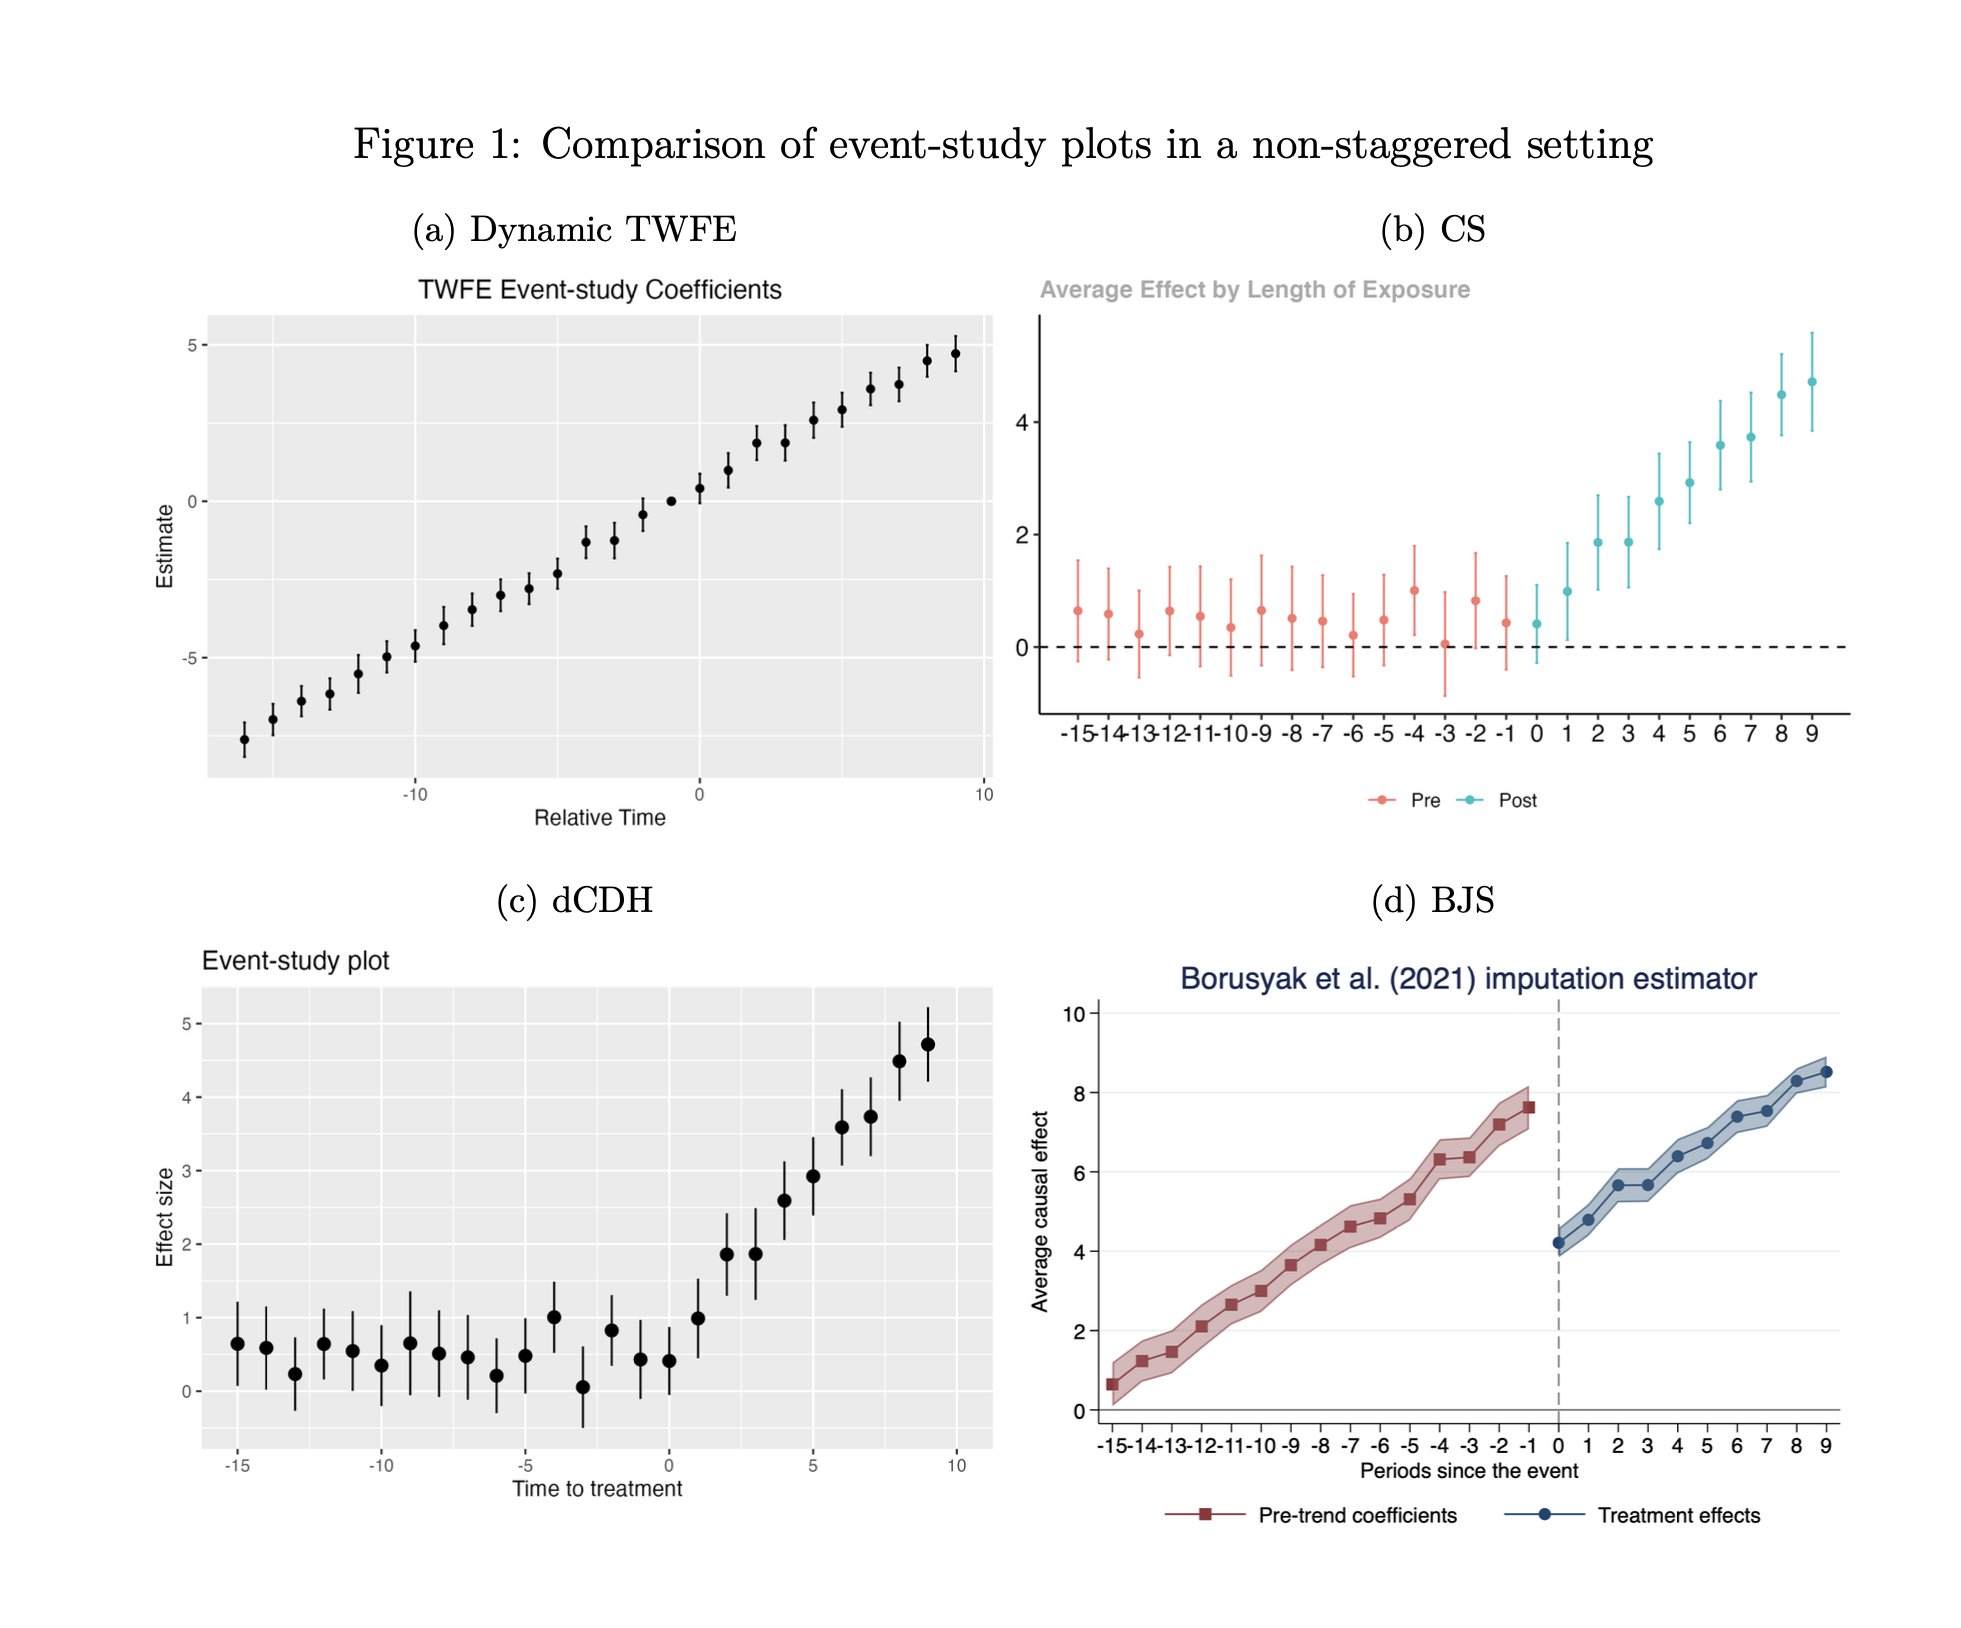
\includegraphics[width=\linewidth, height=0.8\textheight, keepaspectratio]{./lecture_includes/shortgap}
\end{figure}

\end{frame}

\begin{frame}{Stata Syntax}

\begin{itemize}

\item Stata's \texttt{csdid} has default syntax where if you don't indicate which way to do it, it only does it using the short gap method
\item And in the Stata user command from Stata 18, you actually \textbf{cannot} do short differences 
\item You have to select \texttt{long2} in \texttt{csdid} and if you want short gaps, you do not specify anything
\item So what is going on is that since it's not documented well, \texttt{csdid} is very population, and default is short gaps, people are using short gaps and probably don't know, and don't explain it in the papers
\item Here is an NBER that clearly uses short gaps -- with my hand I'll show you the long difference version of the same thing
\end{itemize}

\end{frame}




\begin{frame}

\begin{figure}
    \centering
    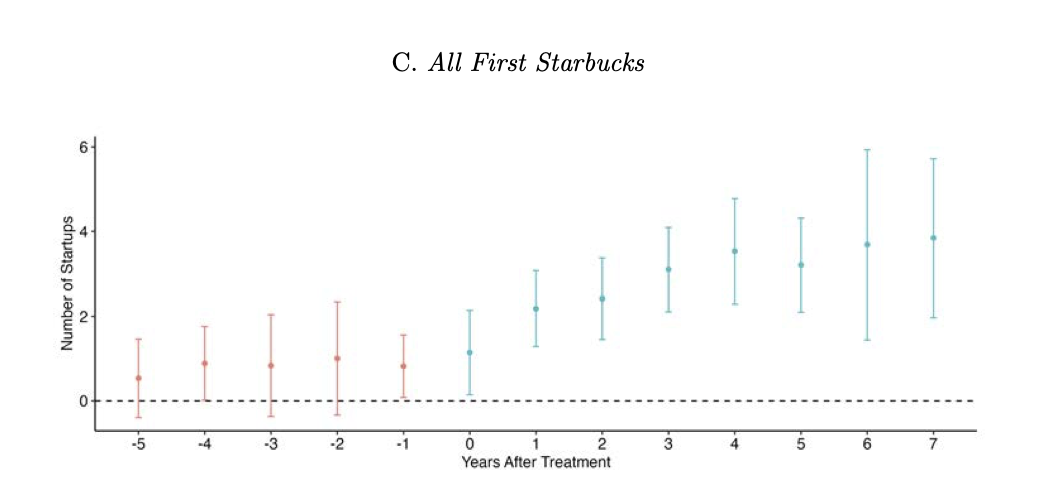
\includegraphics[height=0.5\textheight]{./lecture_includes/magic_johnson_eventstudy}
\end{figure}

\end{frame}


\section{Checklists and My Online Dating Project}


\begin{frame}{How Checklists Saved Lives in Medicine}
    \textbf{Key Idea:} Checklists reduce errors and improve patient safety by standardizing procedures and preventing overlooked steps.

    \begin{itemize}
        \item 
	\textit{The Checklist Manifesto} by Atul Gawande explores how checklists improve outcomes in medicine, aviation, and other fields.
        \item 
	The WHO Surgical Safety Checklist reduced complications and mortality in surgeries worldwide. A study found a 36\% reduction in major surgical complications.
        \item 
	Checklists are thought to work because they:
        \begin{itemize}
            \item Ensure that critical steps are not skipped.
            \item Encourage teamwork and communication.
            \item Create a structured, repeatable process for complex tasks.
        \end{itemize}
    \end{itemize}


\end{frame}


\begin{frame}{Power to the Platform}

\begin{itemize}
\item I'm going to now walk you through a simple checklist I have in my new book
\item Got this from Roth (2022), Pedro Sant'Anna informal conversations, principles from Rubin (2008) and many of Guido Imbens' survey articles
\item We ran into a lot of problems by following this checklist, and a lot of heartbreak followed by excitement
\item It's a study of online dating's effect on the American family, but I'll just focus on birth rates
\item We have a great title -- Power the Platform -- as a homage to "Power to the Pill" by Goldin and Katz and "More Power to the Pill" by Bailey
\end{itemize}

\end{frame}





\begin{frame}{Online Dating and Birth Rates}

\begin{itemize}
\item Me, Christine Durrance, and Melanie Guldi have been working on a project for years looking at online dating's effect on birth rates
	\begin{itemize}
	\item Thickening of relationship markets
	\item Reduced search costs
	\item Formation of better relationships meant for forming families
	\end{itemize}
\item But online dating companies have an incentive to perpetuate dating despite claims to the contrary, which may reduce the formation of families
\end{itemize}
\end{frame}


\begin{frame}

\begin{figure}
    \centering
    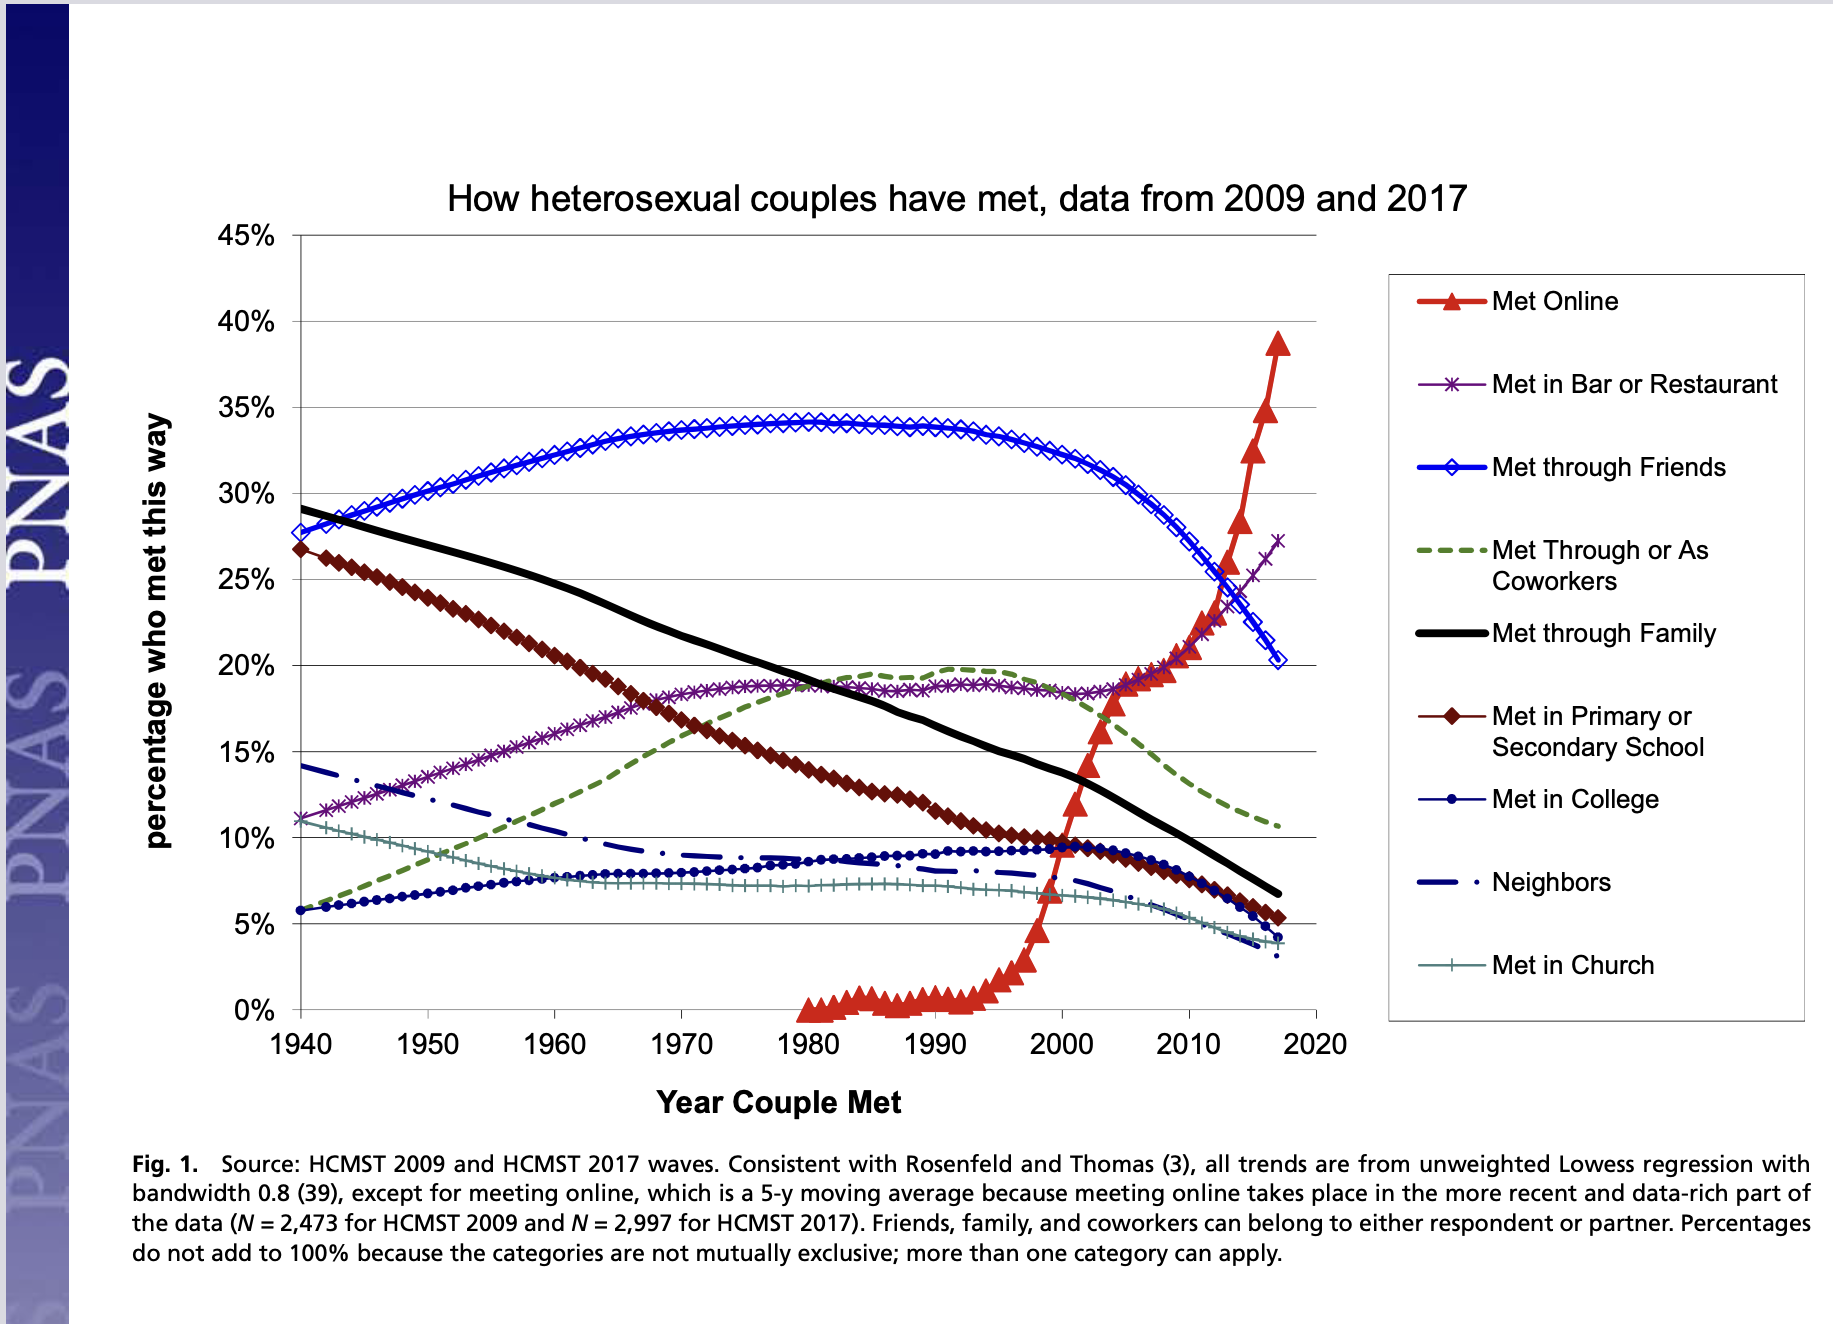
\includegraphics[height=0.85\textheight]{./lecture_includes/online_dating}
\end{figure}

\end{frame}

\begin{frame}{Confounders}

\begin{itemize}

\item Two problems:
	\begin{enumerate}
	\item Online dating either hits the US with an open website anyone can get on (early period) or a "swiping app" that anyone can get on (late period)
	\item After 2008, the American economy birth rates plummeted and never recovered (demographic transition)
	\end{enumerate}
\item Both are massive hurricane like winds and it's going to be challenging to deal with them with diff-in-diff
\item But, amazingly, we have a solution that gets at both and is probably much closer to our target parameter -- Craigslist Personals

\end{itemize}

\end{frame}

\begin{frame}{What was Craigslist Personals?}

\begin{itemize}
\item Craigslist is one of the most visited websites in the United States
\item Two sided matching website that devastated classified advertising revenue in newspapers
\item Primarily made money from housing and jobs, but you can get \emph{anything} on it 
\end{itemize}

\end{frame}

\begin{frame}{What was Craigslist Personals?}

\begin{itemize}
\item But then in 2000, in the Bay Area (i.e., San Francisco), they introduce "People matching technology" (their words) 
\item Casual sex, serious relationships, men seeking men, men seeking women, women seeking men, women seeking men
\item And great for us -- cities got this on different dates giving us "staggered rollout" 
\end{itemize}

\end{frame}









\begin{frame}{Personals}

\begin{figure}
    \centering
    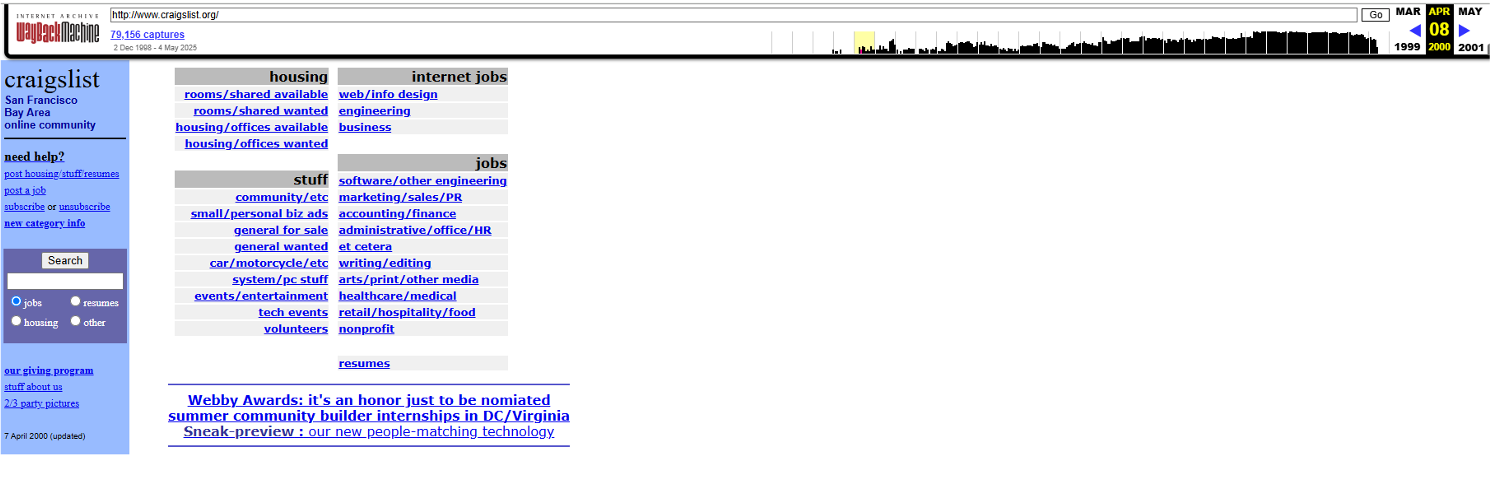
\includegraphics[height=0.85\textheight]{./lecture_includes/melanie1}
\end{figure}

\end{frame}


\begin{frame}{Personals}
\begin{figure}
    \centering
    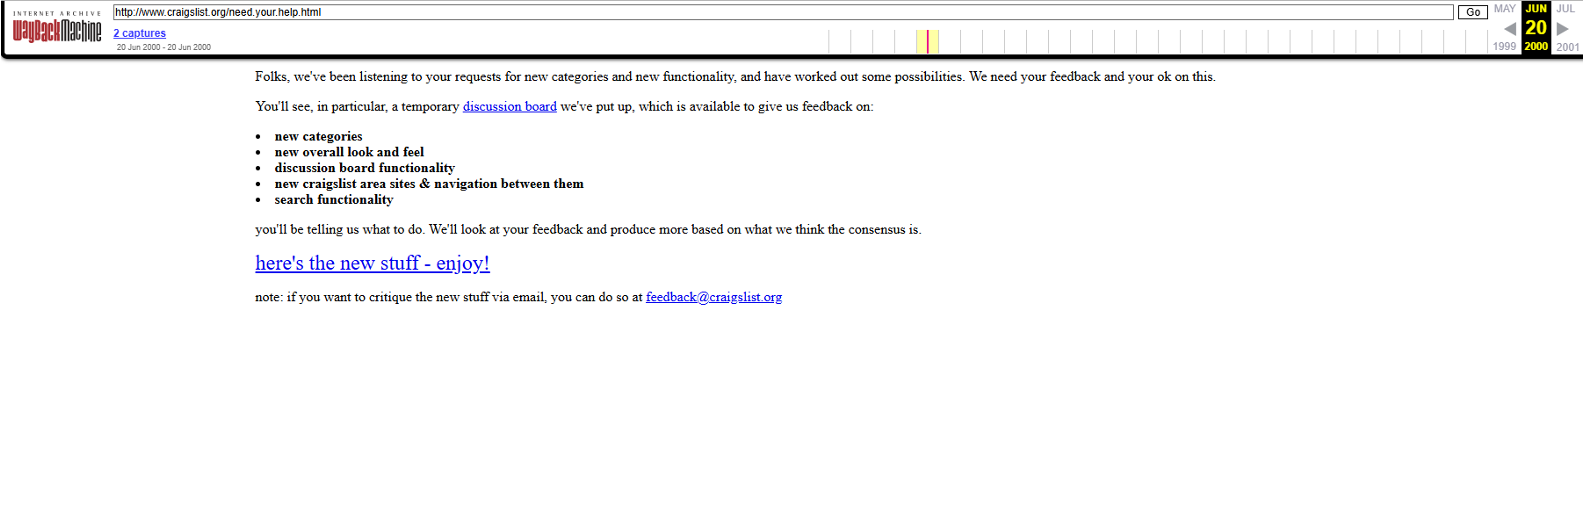
\includegraphics[height=0.5\textheight]{./lecture_includes/melanie2}
\end{figure}

\end{frame}

\begin{frame}{Personals starts in San Francisco}
\begin{figure}
    \centering
    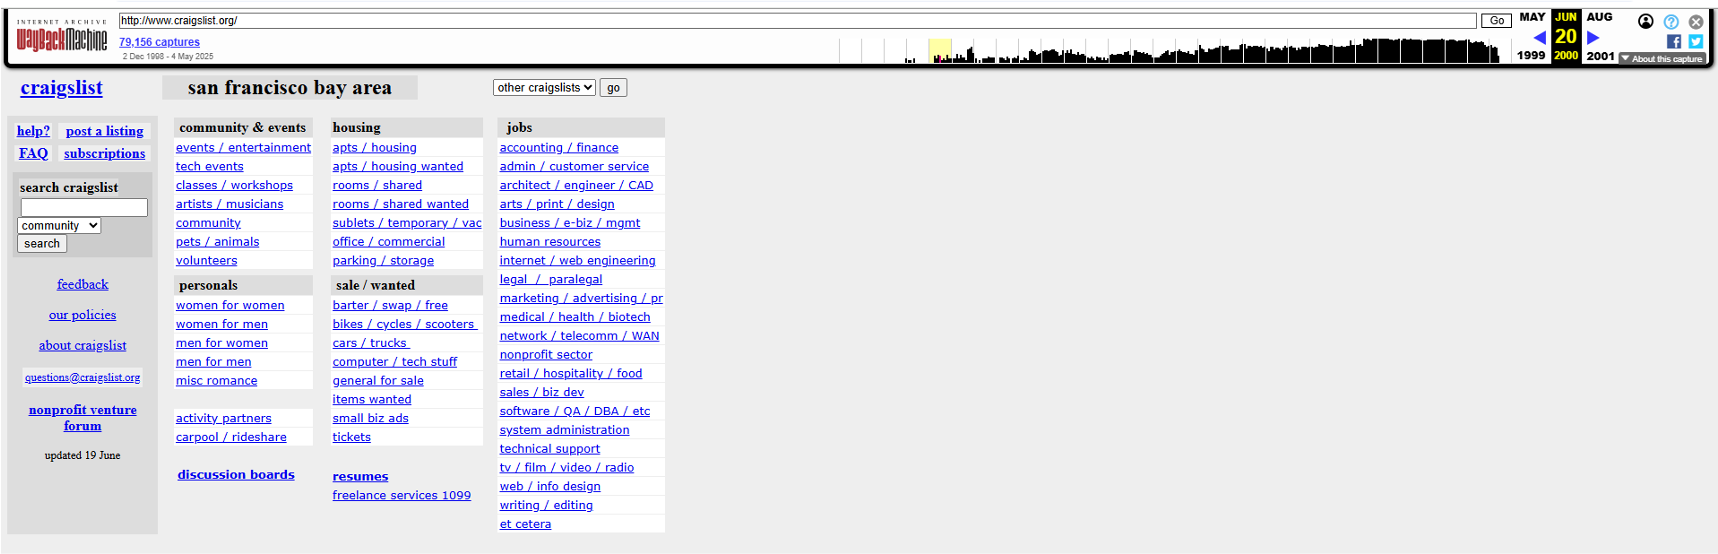
\includegraphics[height=0.85\textheight]{./lecture_includes/melanie3}
\end{figure}

\end{frame}

\begin{frame}{Personals begins spreading}
\begin{figure}
    \centering
    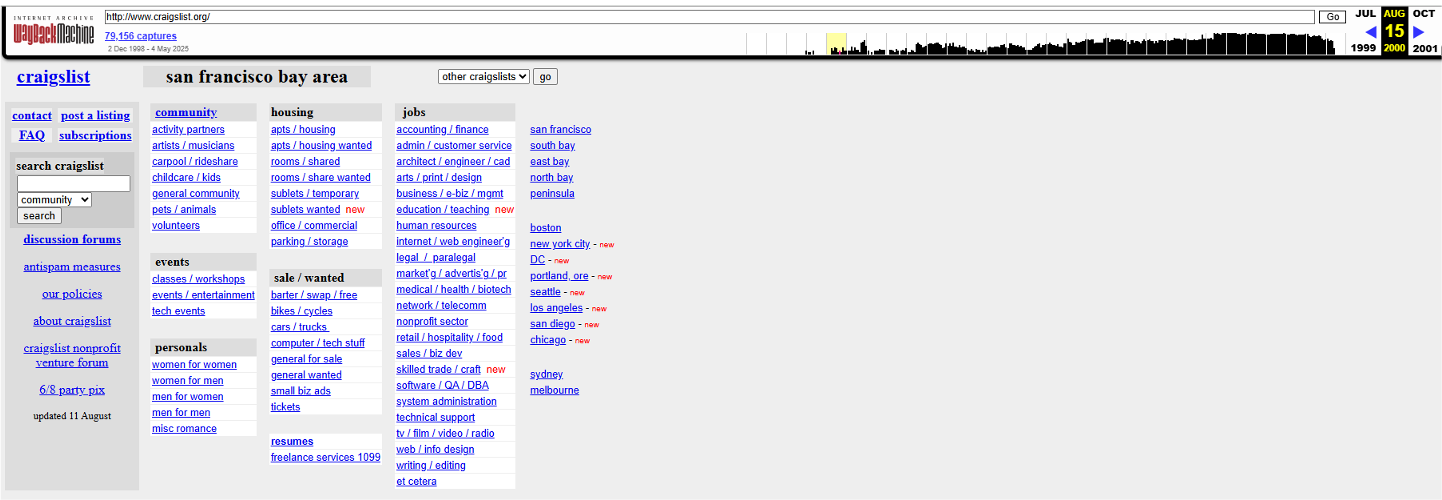
\includegraphics[height=0.85\textheight]{./lecture_includes/melanie4}
\end{figure}

\end{frame}

\begin{frame}{Personals gets larger}
\begin{figure}
    \centering
    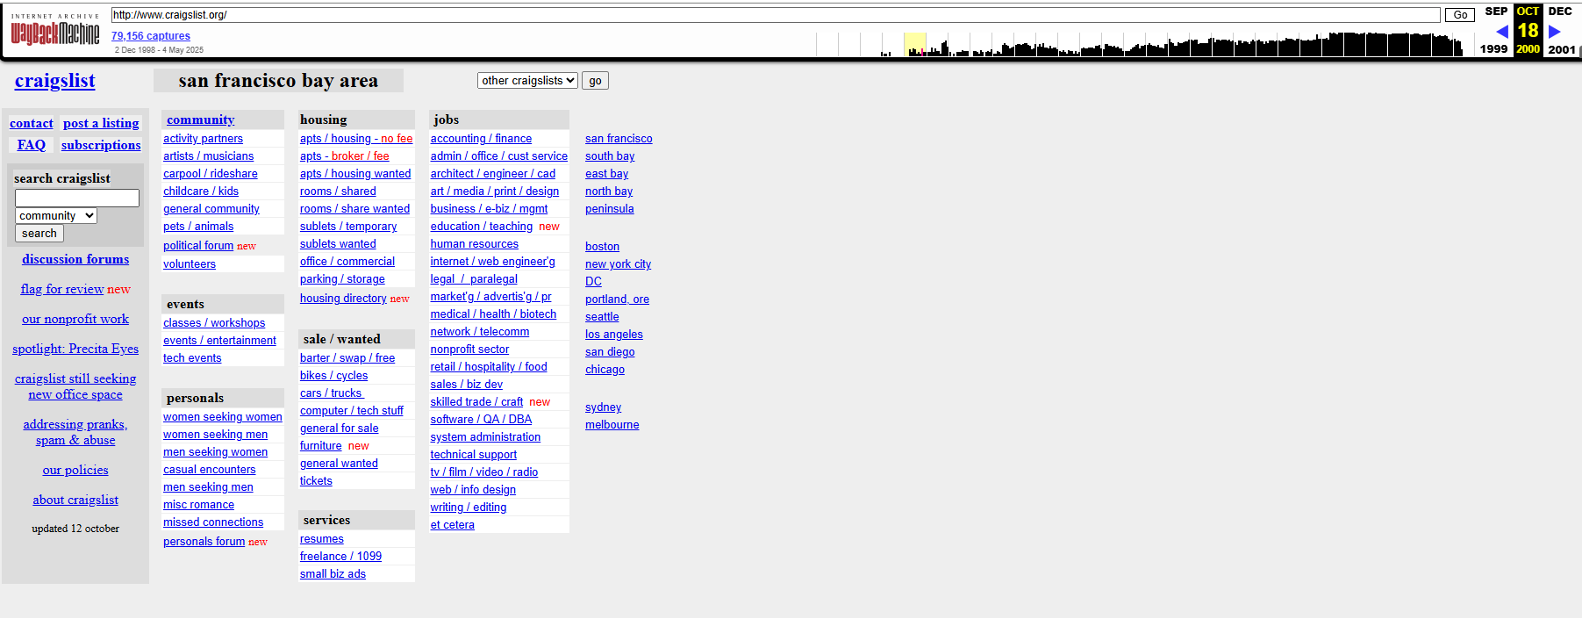
\includegraphics[height=0.85\textheight]{./lecture_includes/melanie5}
\end{figure}

\end{frame}

\begin{frame}{Personals is popular!}
\begin{figure}
    \centering
    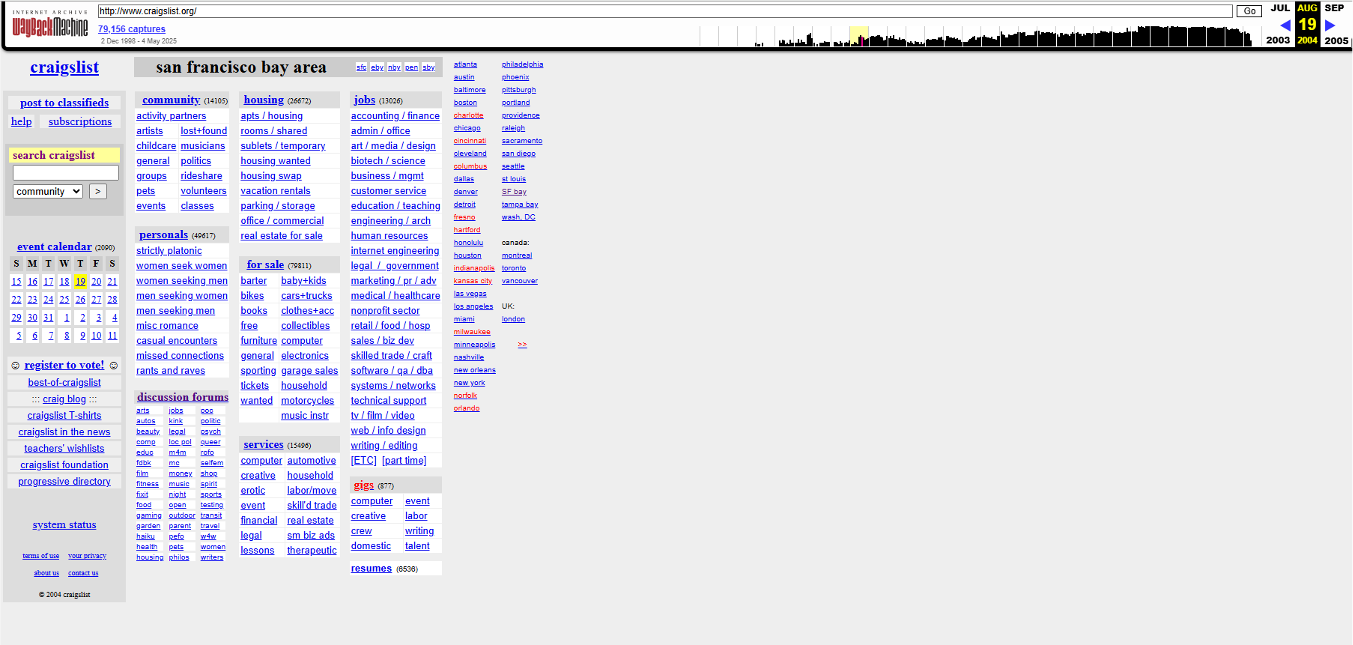
\includegraphics[height=0.85\textheight]{./lecture_includes/melanie6}
\end{figure}

\end{frame}

\begin{frame}{Personals is popular!}
\begin{figure}
    \centering
    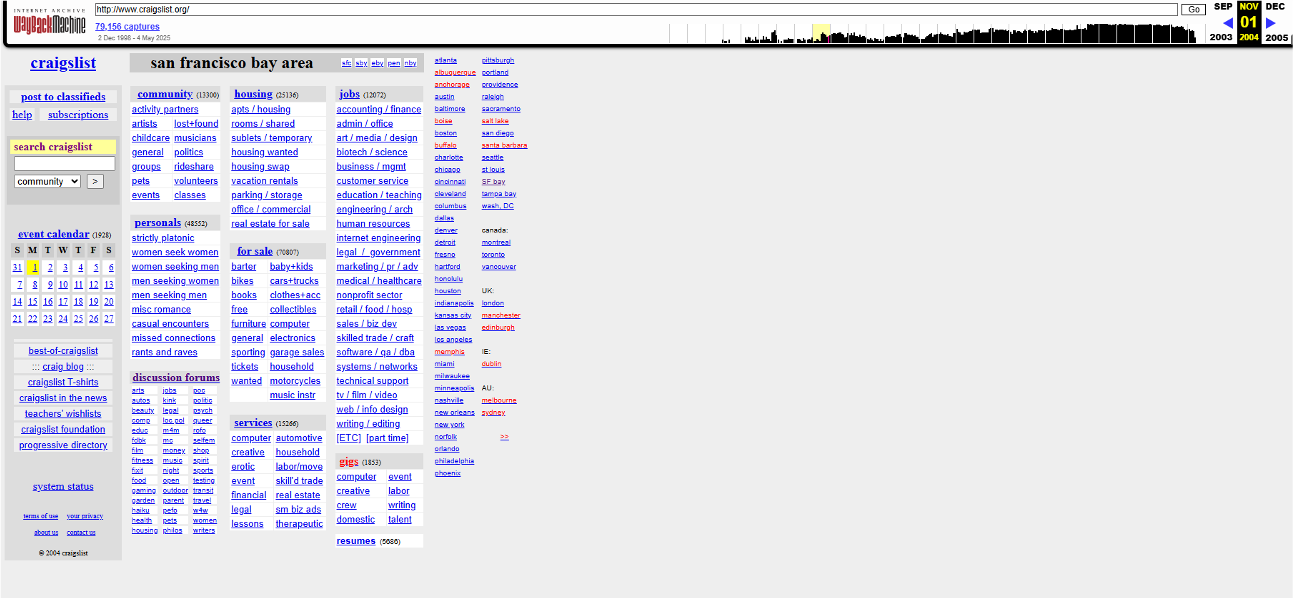
\includegraphics[height=0.85\textheight]{./lecture_includes/melanie7}
\end{figure}

\end{frame}

\begin{frame}{Personals is popular!}
\begin{figure}
    \centering
    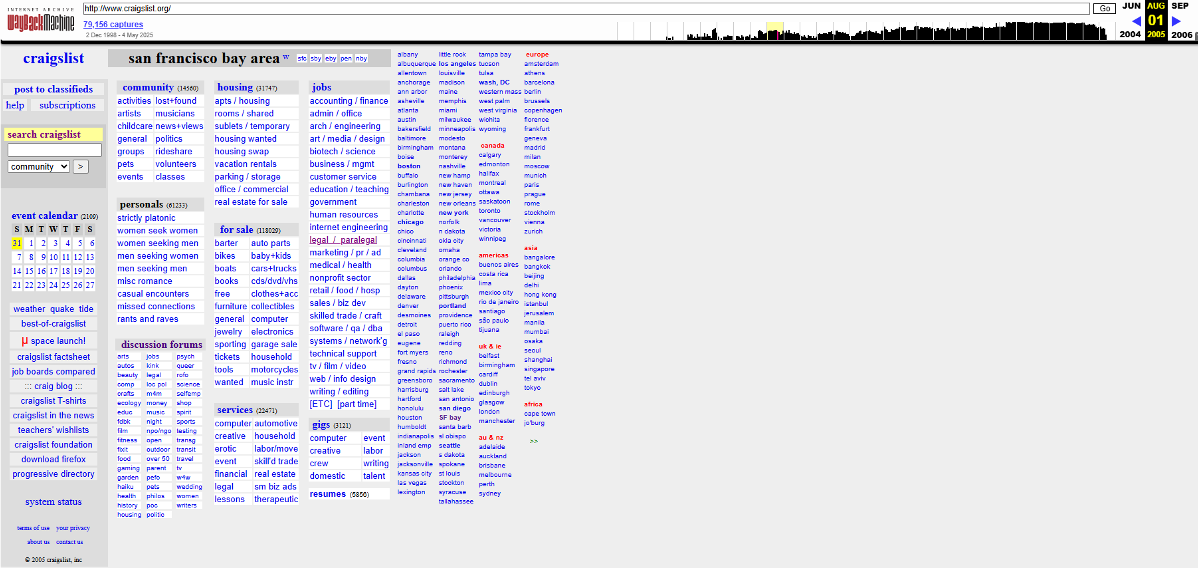
\includegraphics[height=0.85\textheight]{./lecture_includes/melanie8}
\end{figure}

\end{frame}


\begin{frame}{Our project}

\begin{itemize}
\item So we have geographic rollout from 2000 to 2010
	\begin{enumerate}
\item But after 2008, Great Recession leads to plummeting birth rates
\item And after 2008, we have social media, smart phones, all of which maybe had their own independent effects on matching ("sex recessions")
	\end{enumerate}
\item So we will use 1995 (pre-treatment) to 2007 as our sample period
\item But we will include the 2008-2010 "later treated counties" as our control group
\item Used the wayback machine to get every county's craigslist start date (three of us and an RA!)
\end{itemize}

\end{frame}

\begin{frame}{Recovery of Birth Rates (National vs. County)}
    \centering
    \begin{columns}
        \column{0.5\textwidth}
        \centering
        \textbf{Average National Birth Rates}
        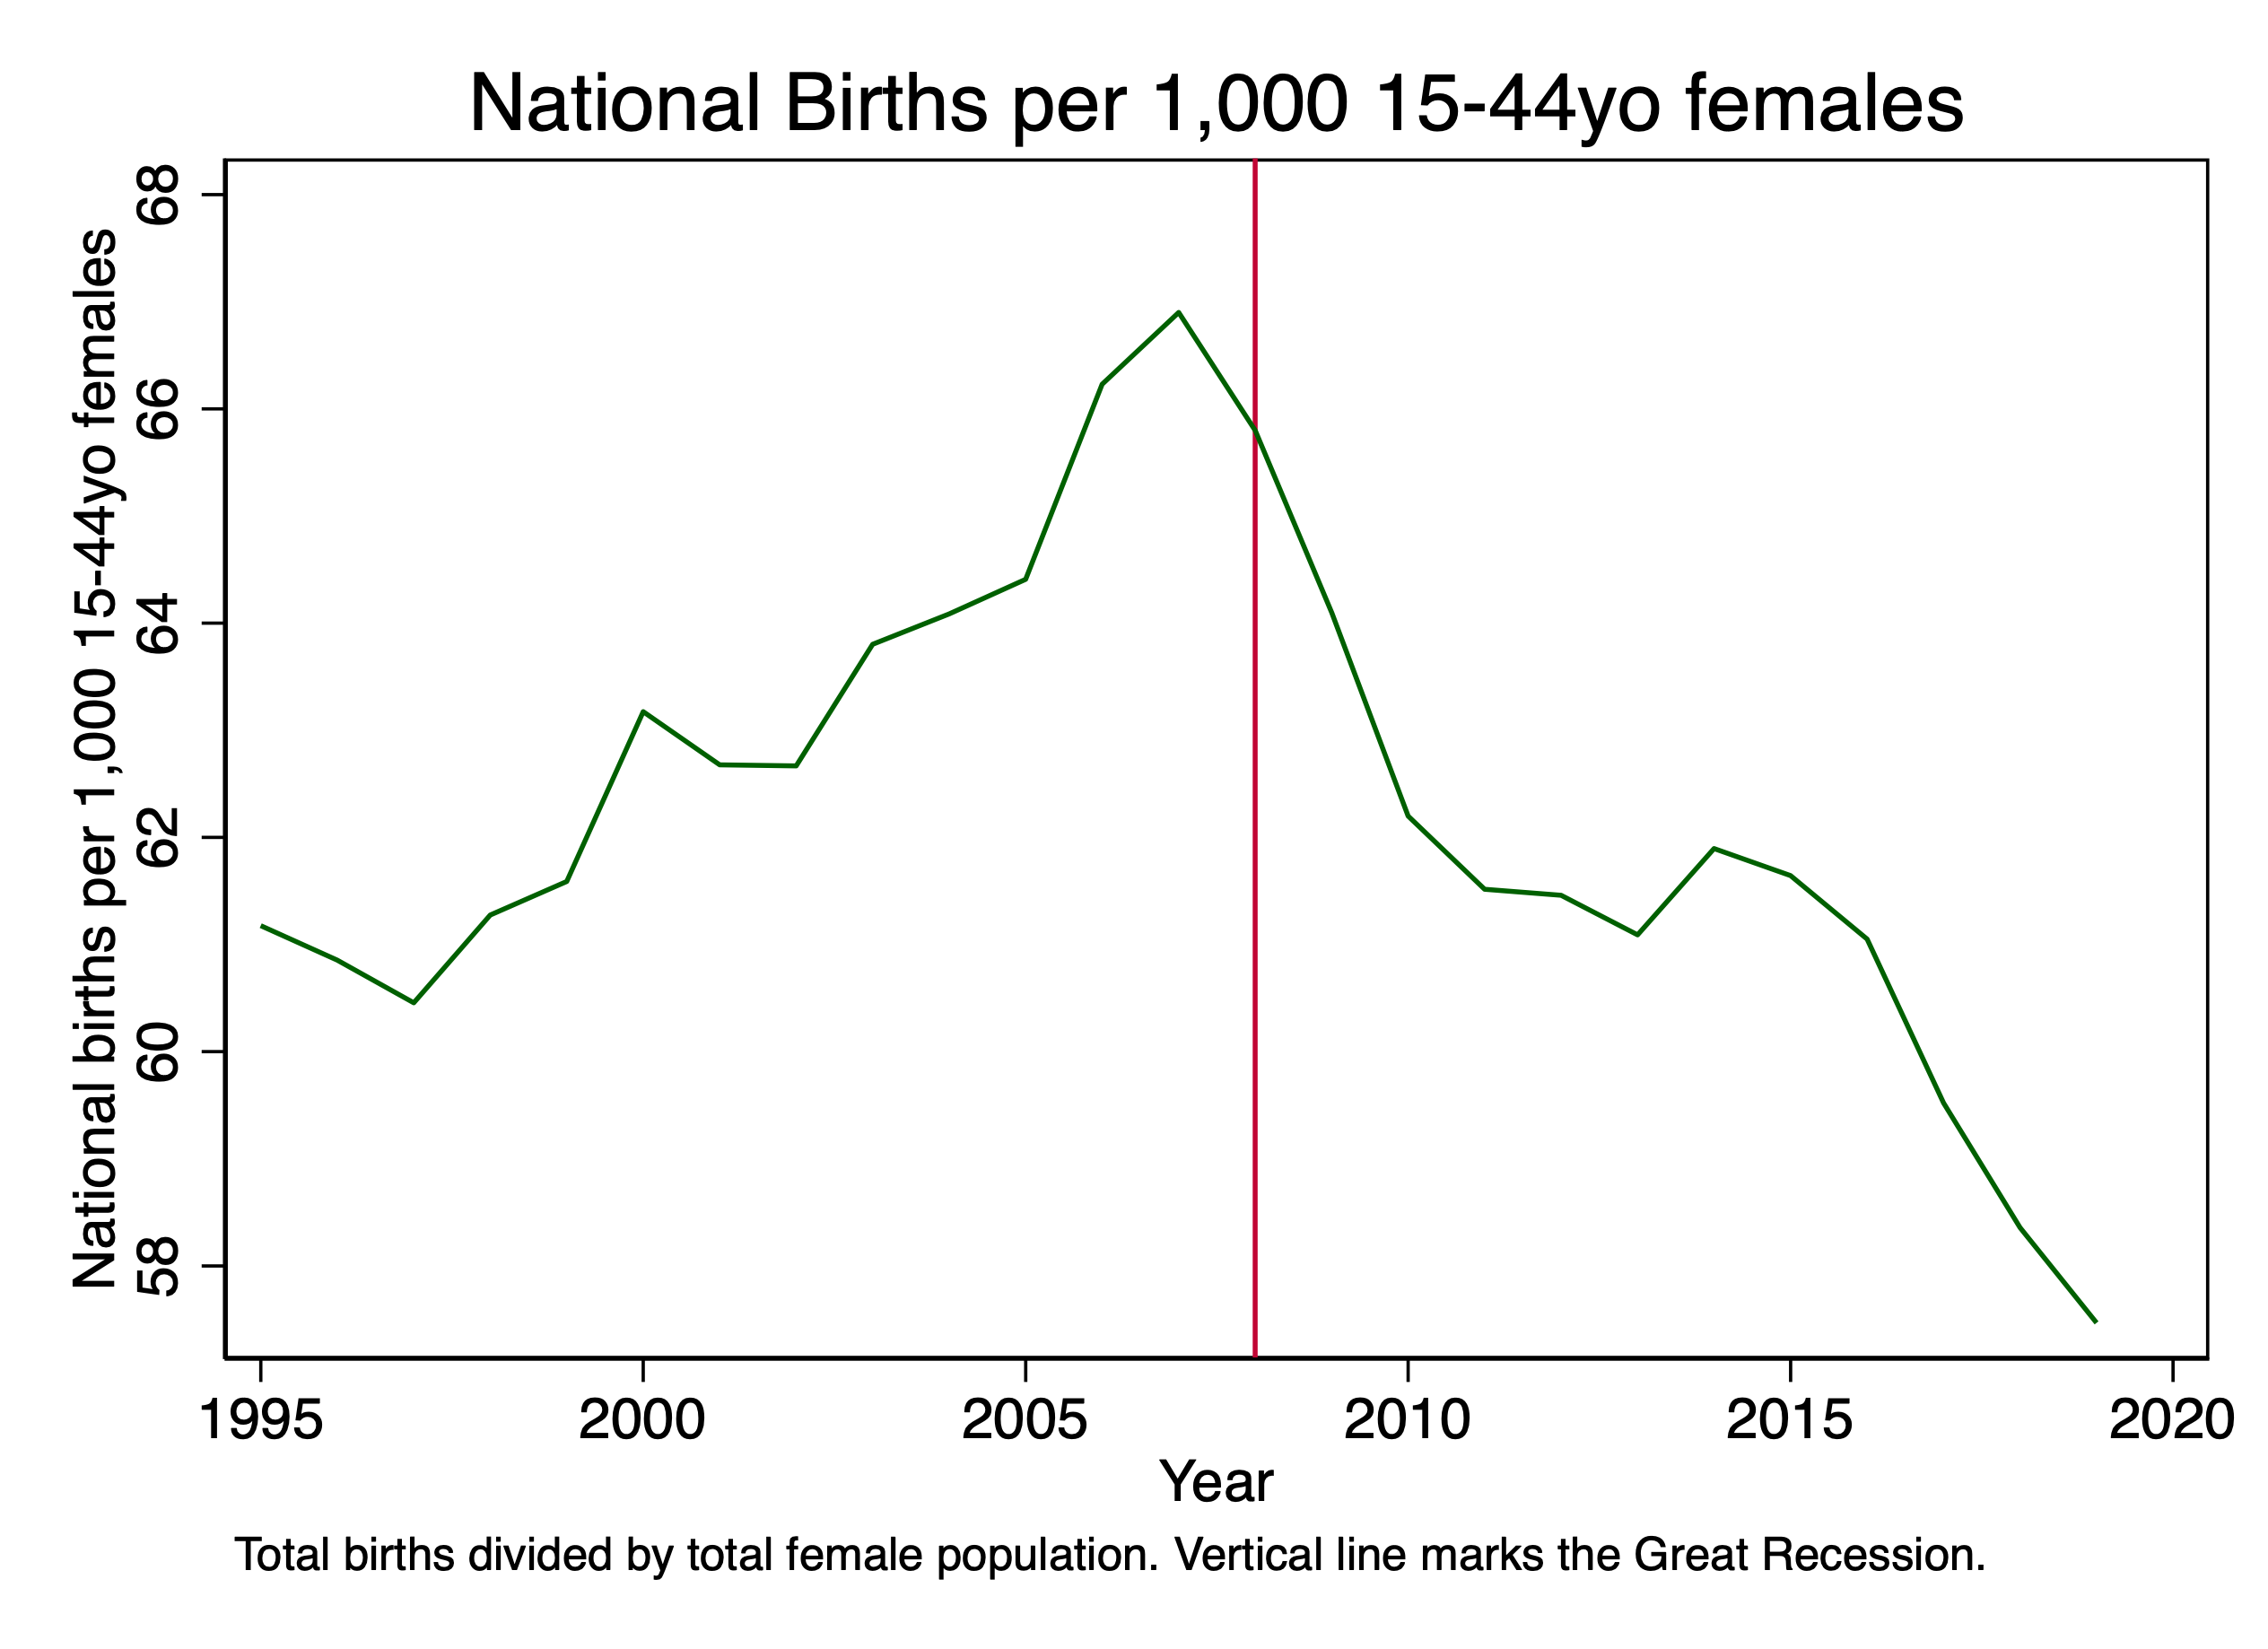
\includegraphics[width=\linewidth,height=0.6\textheight,keepaspectratio]{./lecture_includes/national_br.png}
        
        \column{0.5\textwidth}
        \centering
        \textbf{Average County Birth Rates}
        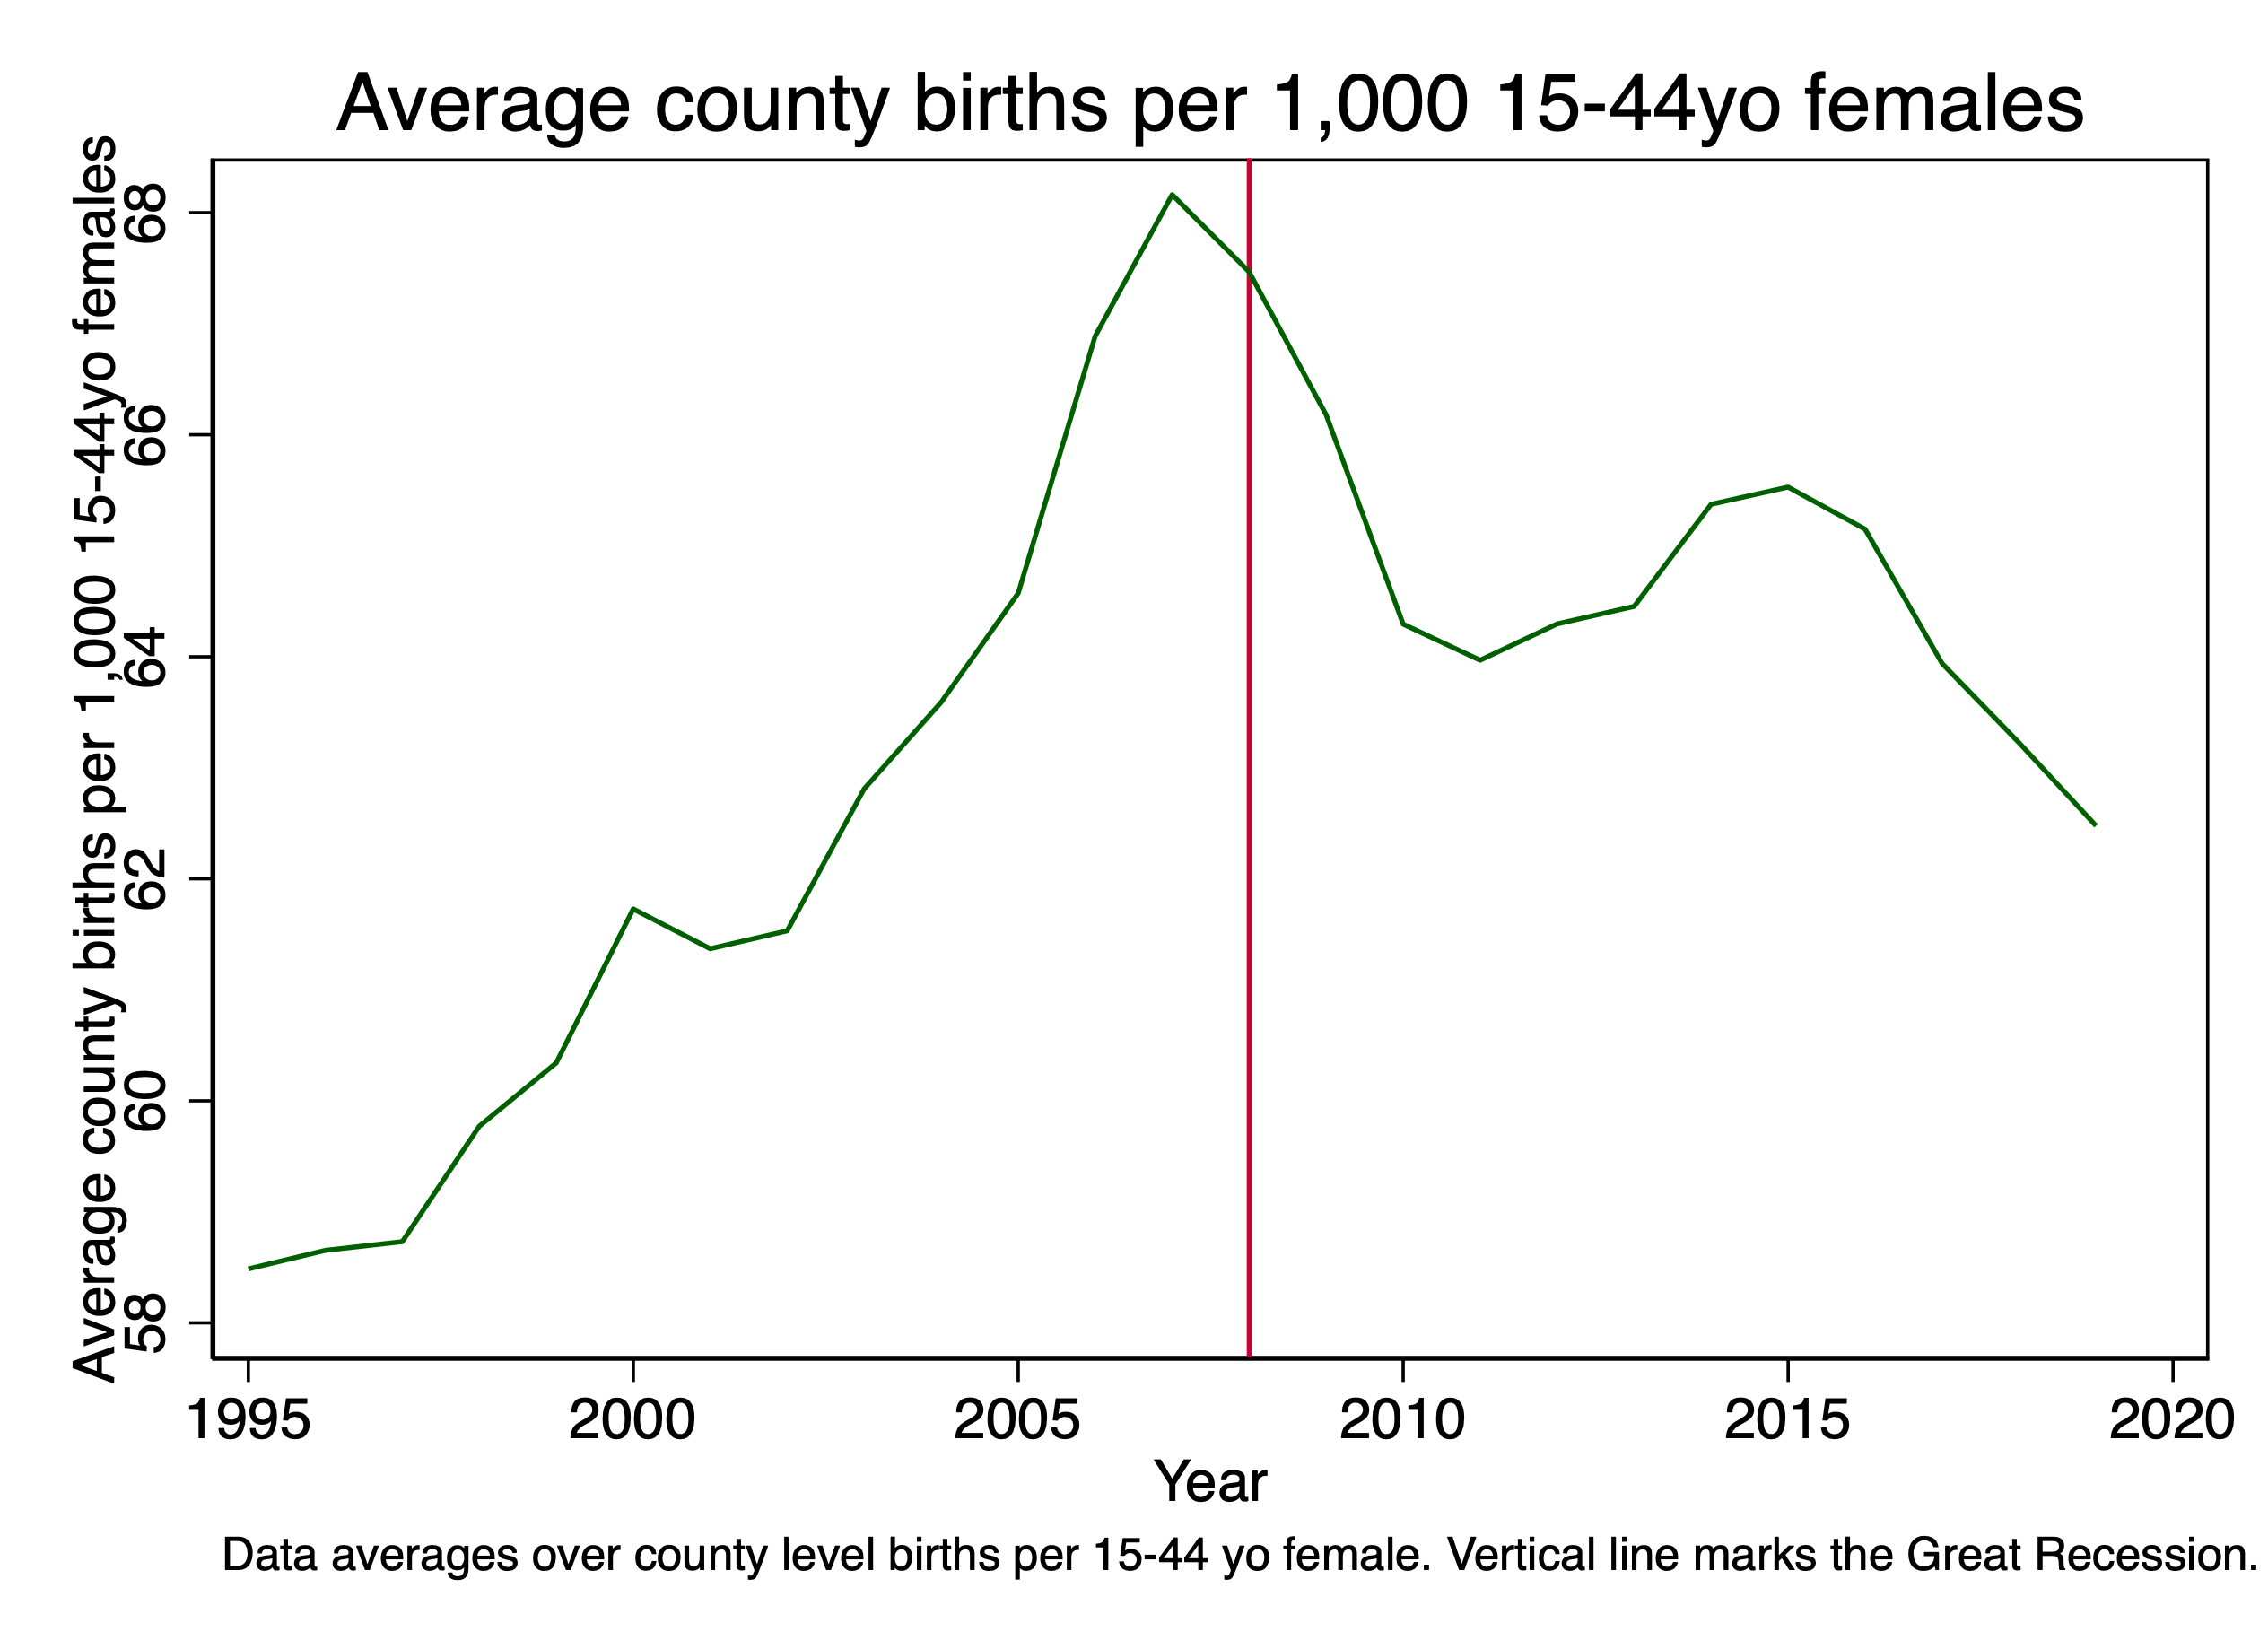
\includegraphics[width=\linewidth,height=0.6\textheight,keepaspectratio]{./lecture_includes/county_br.png}
    \end{columns}
\end{frame}


\begin{frame}

\begin{figure}
    \centering
    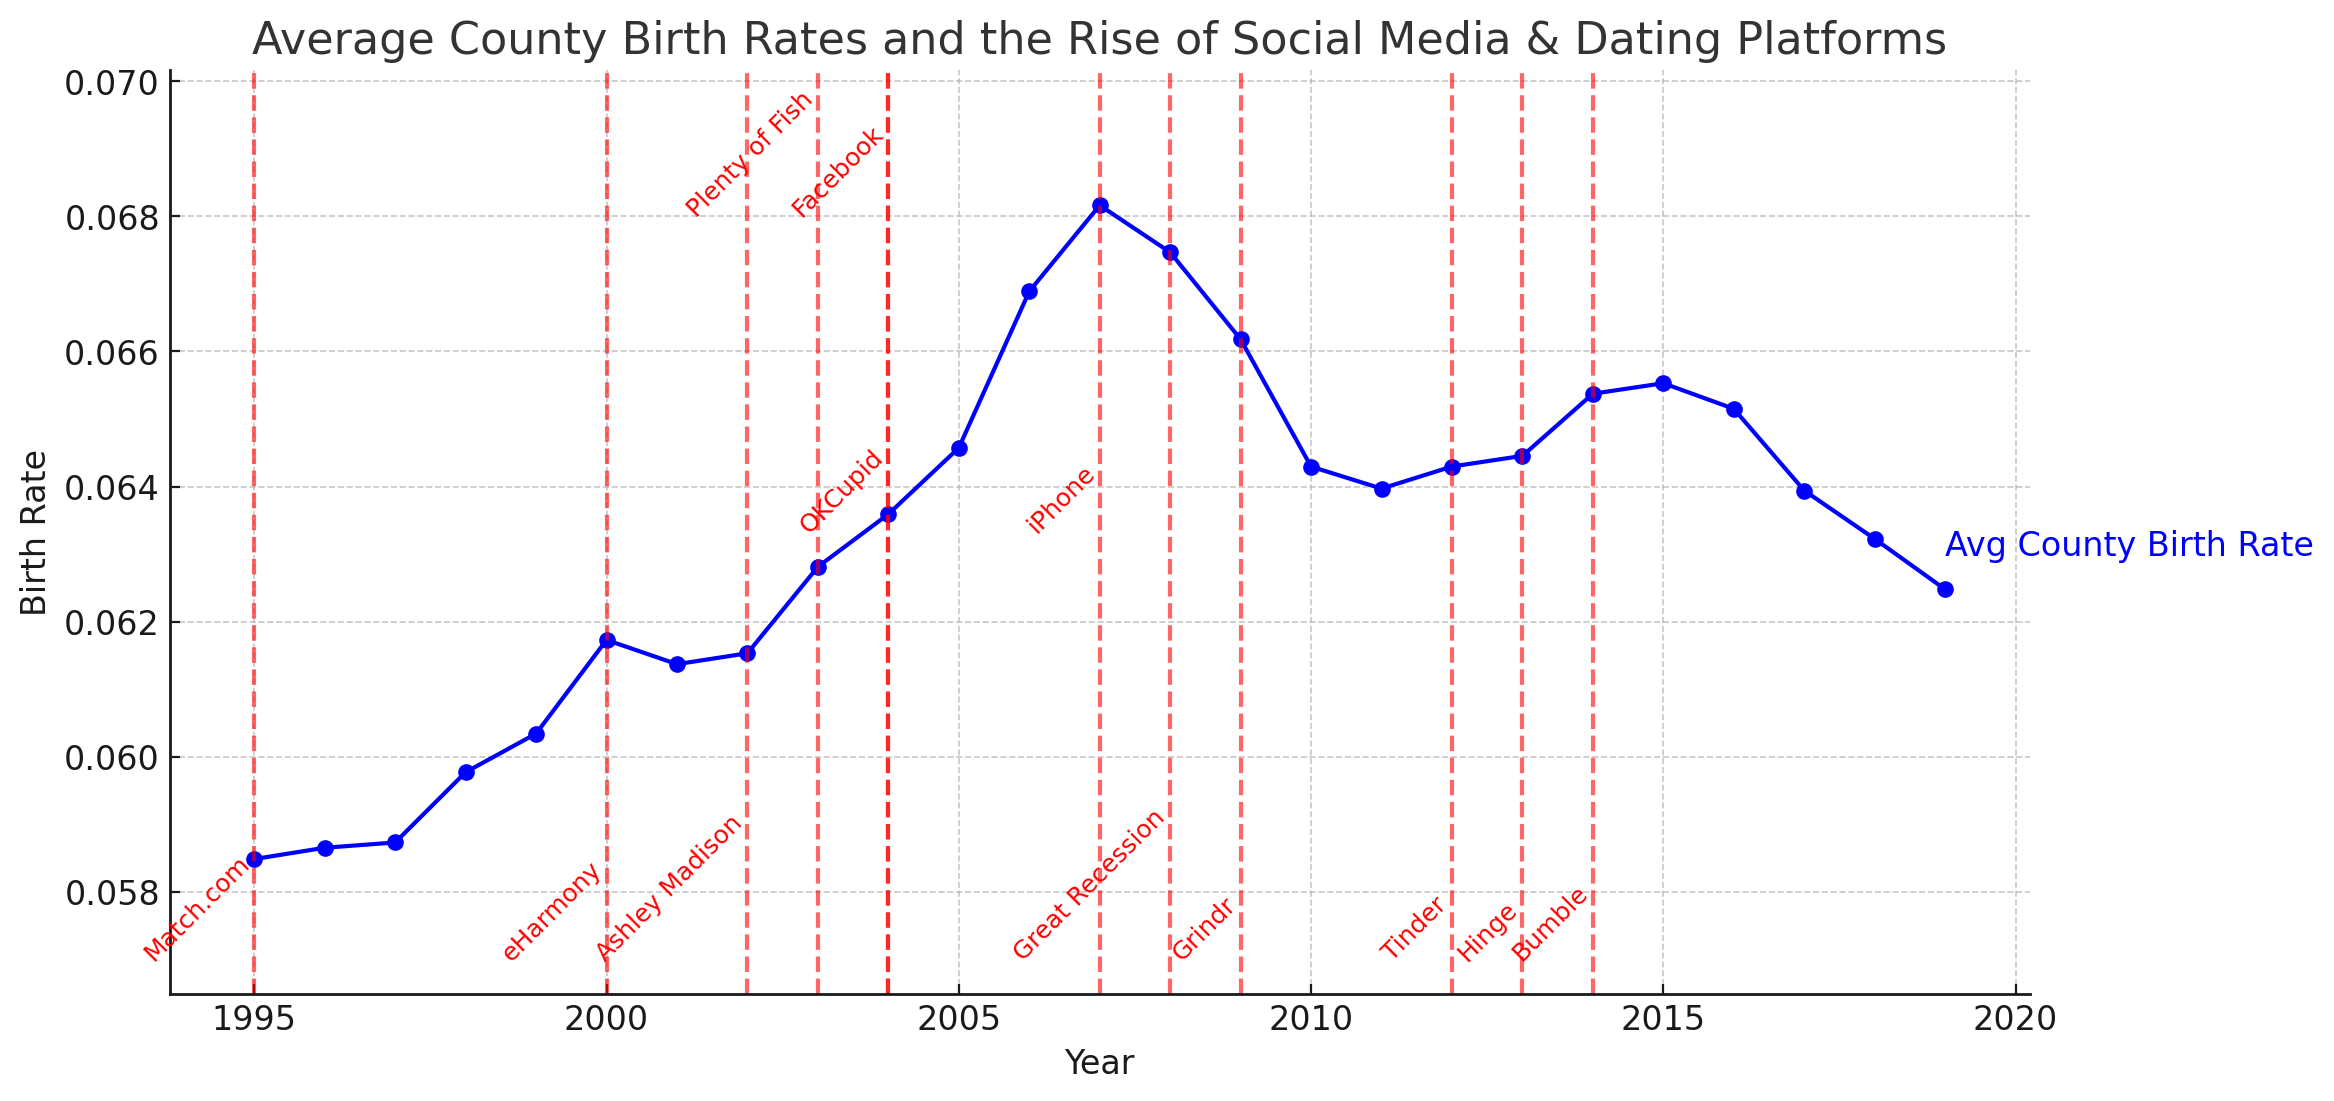
\includegraphics[height=0.6\textheight]{./lecture_includes/python_births.png}
\end{figure}

\end{frame}





\begin{frame}[shrink=20]{Number of counties by treatment cohorts}
\begin{table}[htbp]\centering
\caption{Number of counties by year Craigslist personals appeared}\label{tab:countybycohort}
\begin{tabular}{lc}
\toprule
\textbf{Treatment Cohort} & \textbf{Number of Counties Treated} \\
\midrule
Never treated&       1,779\\
2000 cohort &           9\\
2001 cohort &           5\\
2002 cohort &          12\\
2003 cohort &          36\\
2004 cohort &          58\\
2005 cohort &          69\\
2006 cohort &         341\\
2007 cohort &          65\\
2008 cohort &          66\\
2009 cohort &         215\\
2010 cohort &           1\\
\midrule
Total counties &     2,656 \\
\bottomrule
\end{tabular}
\end{table}
\end{frame}


\begin{frame}{Rollout of Craigslist's Personals}
    \centering
    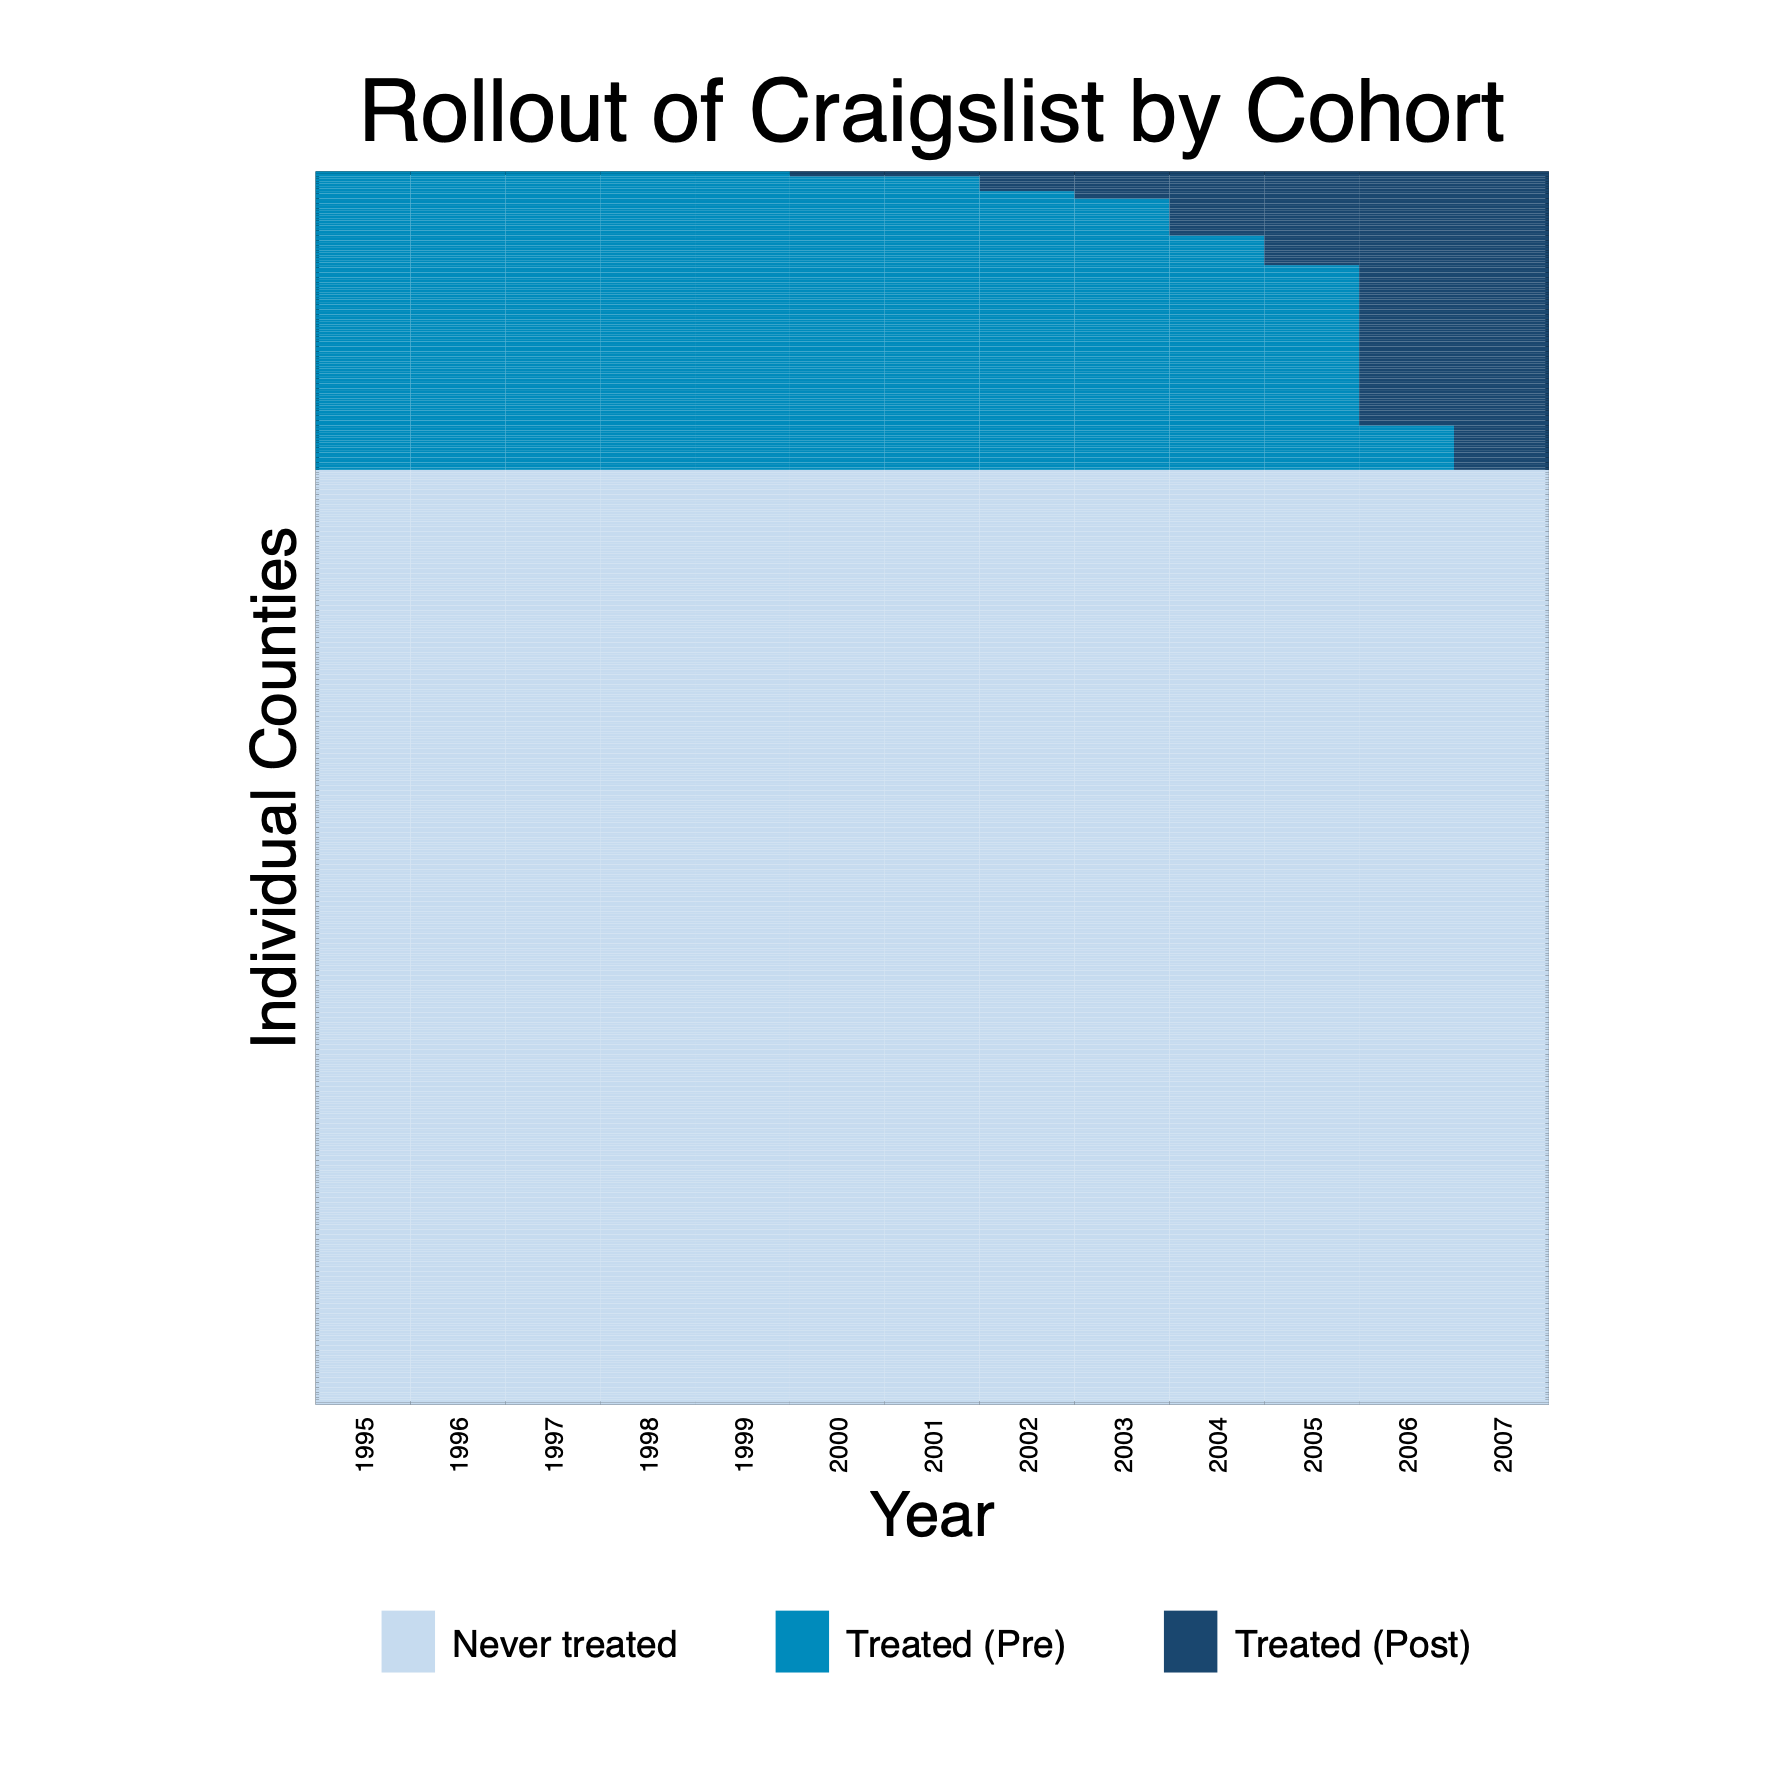
\includegraphics[width=\textwidth,height=0.95\textheight,keepaspectratio]{./lecture_includes/rollout.png}
\end{frame}

\begin{frame}{Births by Treatment Cohort}
    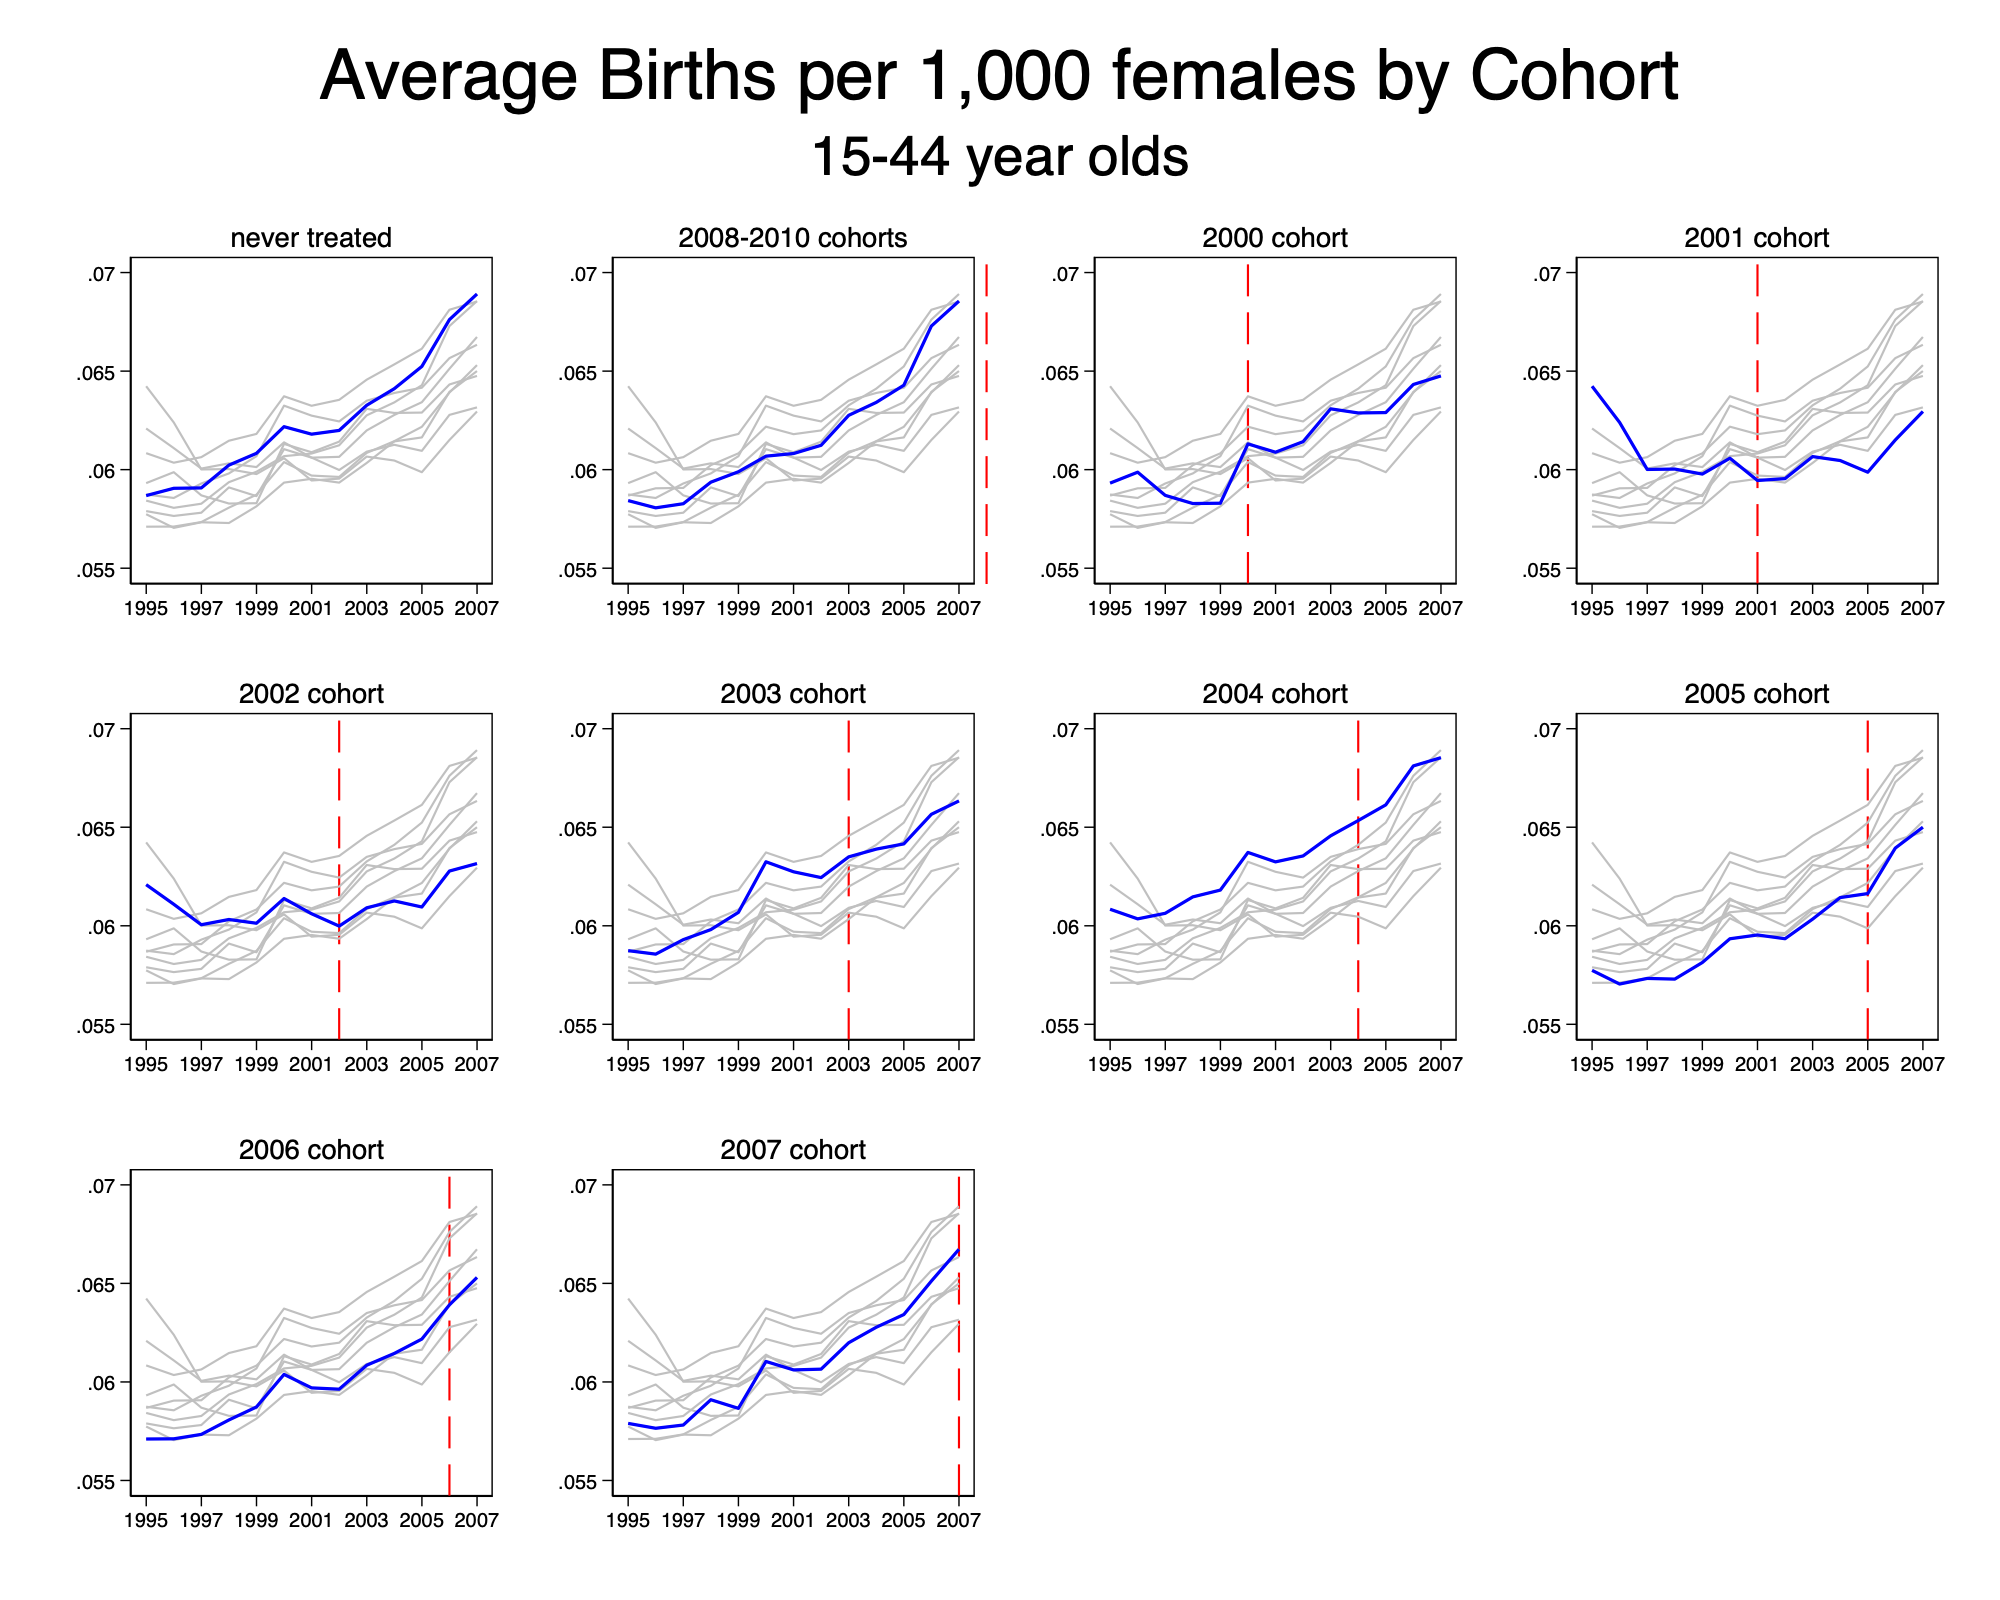
\includegraphics[width=\textwidth,height=0.9\textheight,keepaspectratio]{./lecture_includes/pretty_births.png}
\end{frame}


\begin{frame}{Estimator selection}

\begin{itemize}

\item We used CS to estimate the average effect of the rollout on birth rates 
\item It's unweighted by population so "average effect on the average county for now
\item We decided to make our control group the "2008-2010" as our control group because at least they were eventually treated, but doesn't really matter as never-treated gets same things
\item First, I want to just illustrate for you the "short vs long difference" issue

\end{itemize}

\end{frame}





\begin{frame}{Short gap event study, no covariates}

\begin{figure}
    \centering
    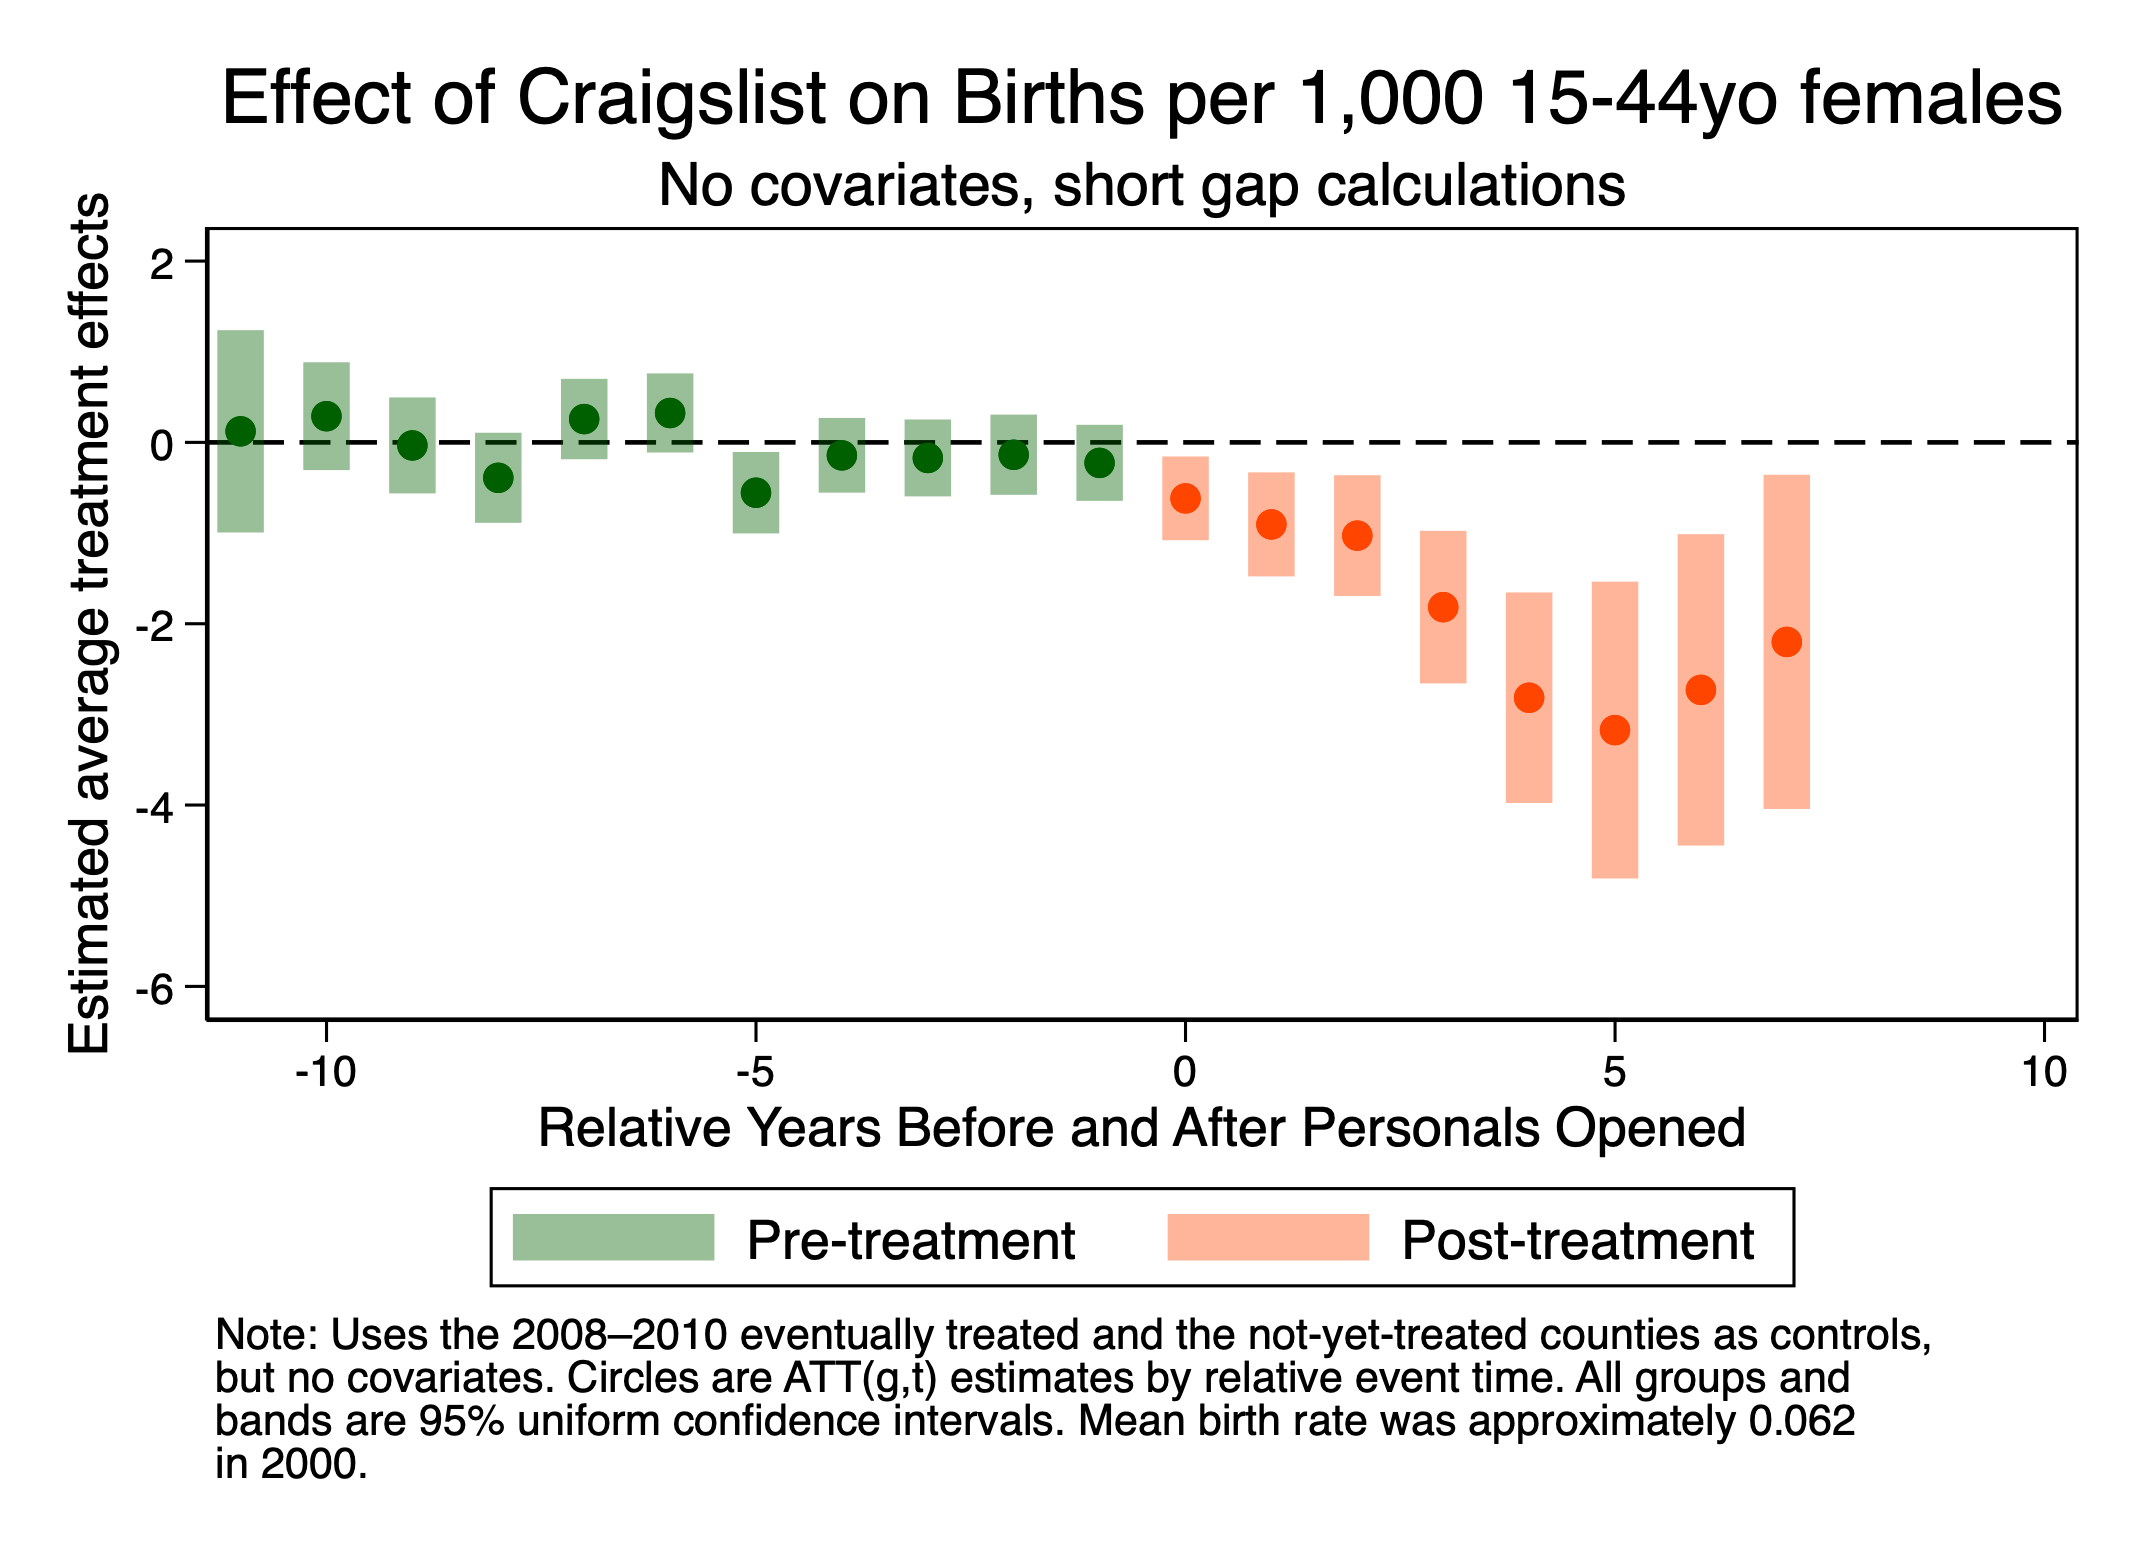
\includegraphics[height=0.85\textheight]{./lecture_includes/es_births_shortnone.png}
\end{figure}

\end{frame}

\begin{frame}{Long differences event study, no covariates}

\begin{figure}
    \centering
    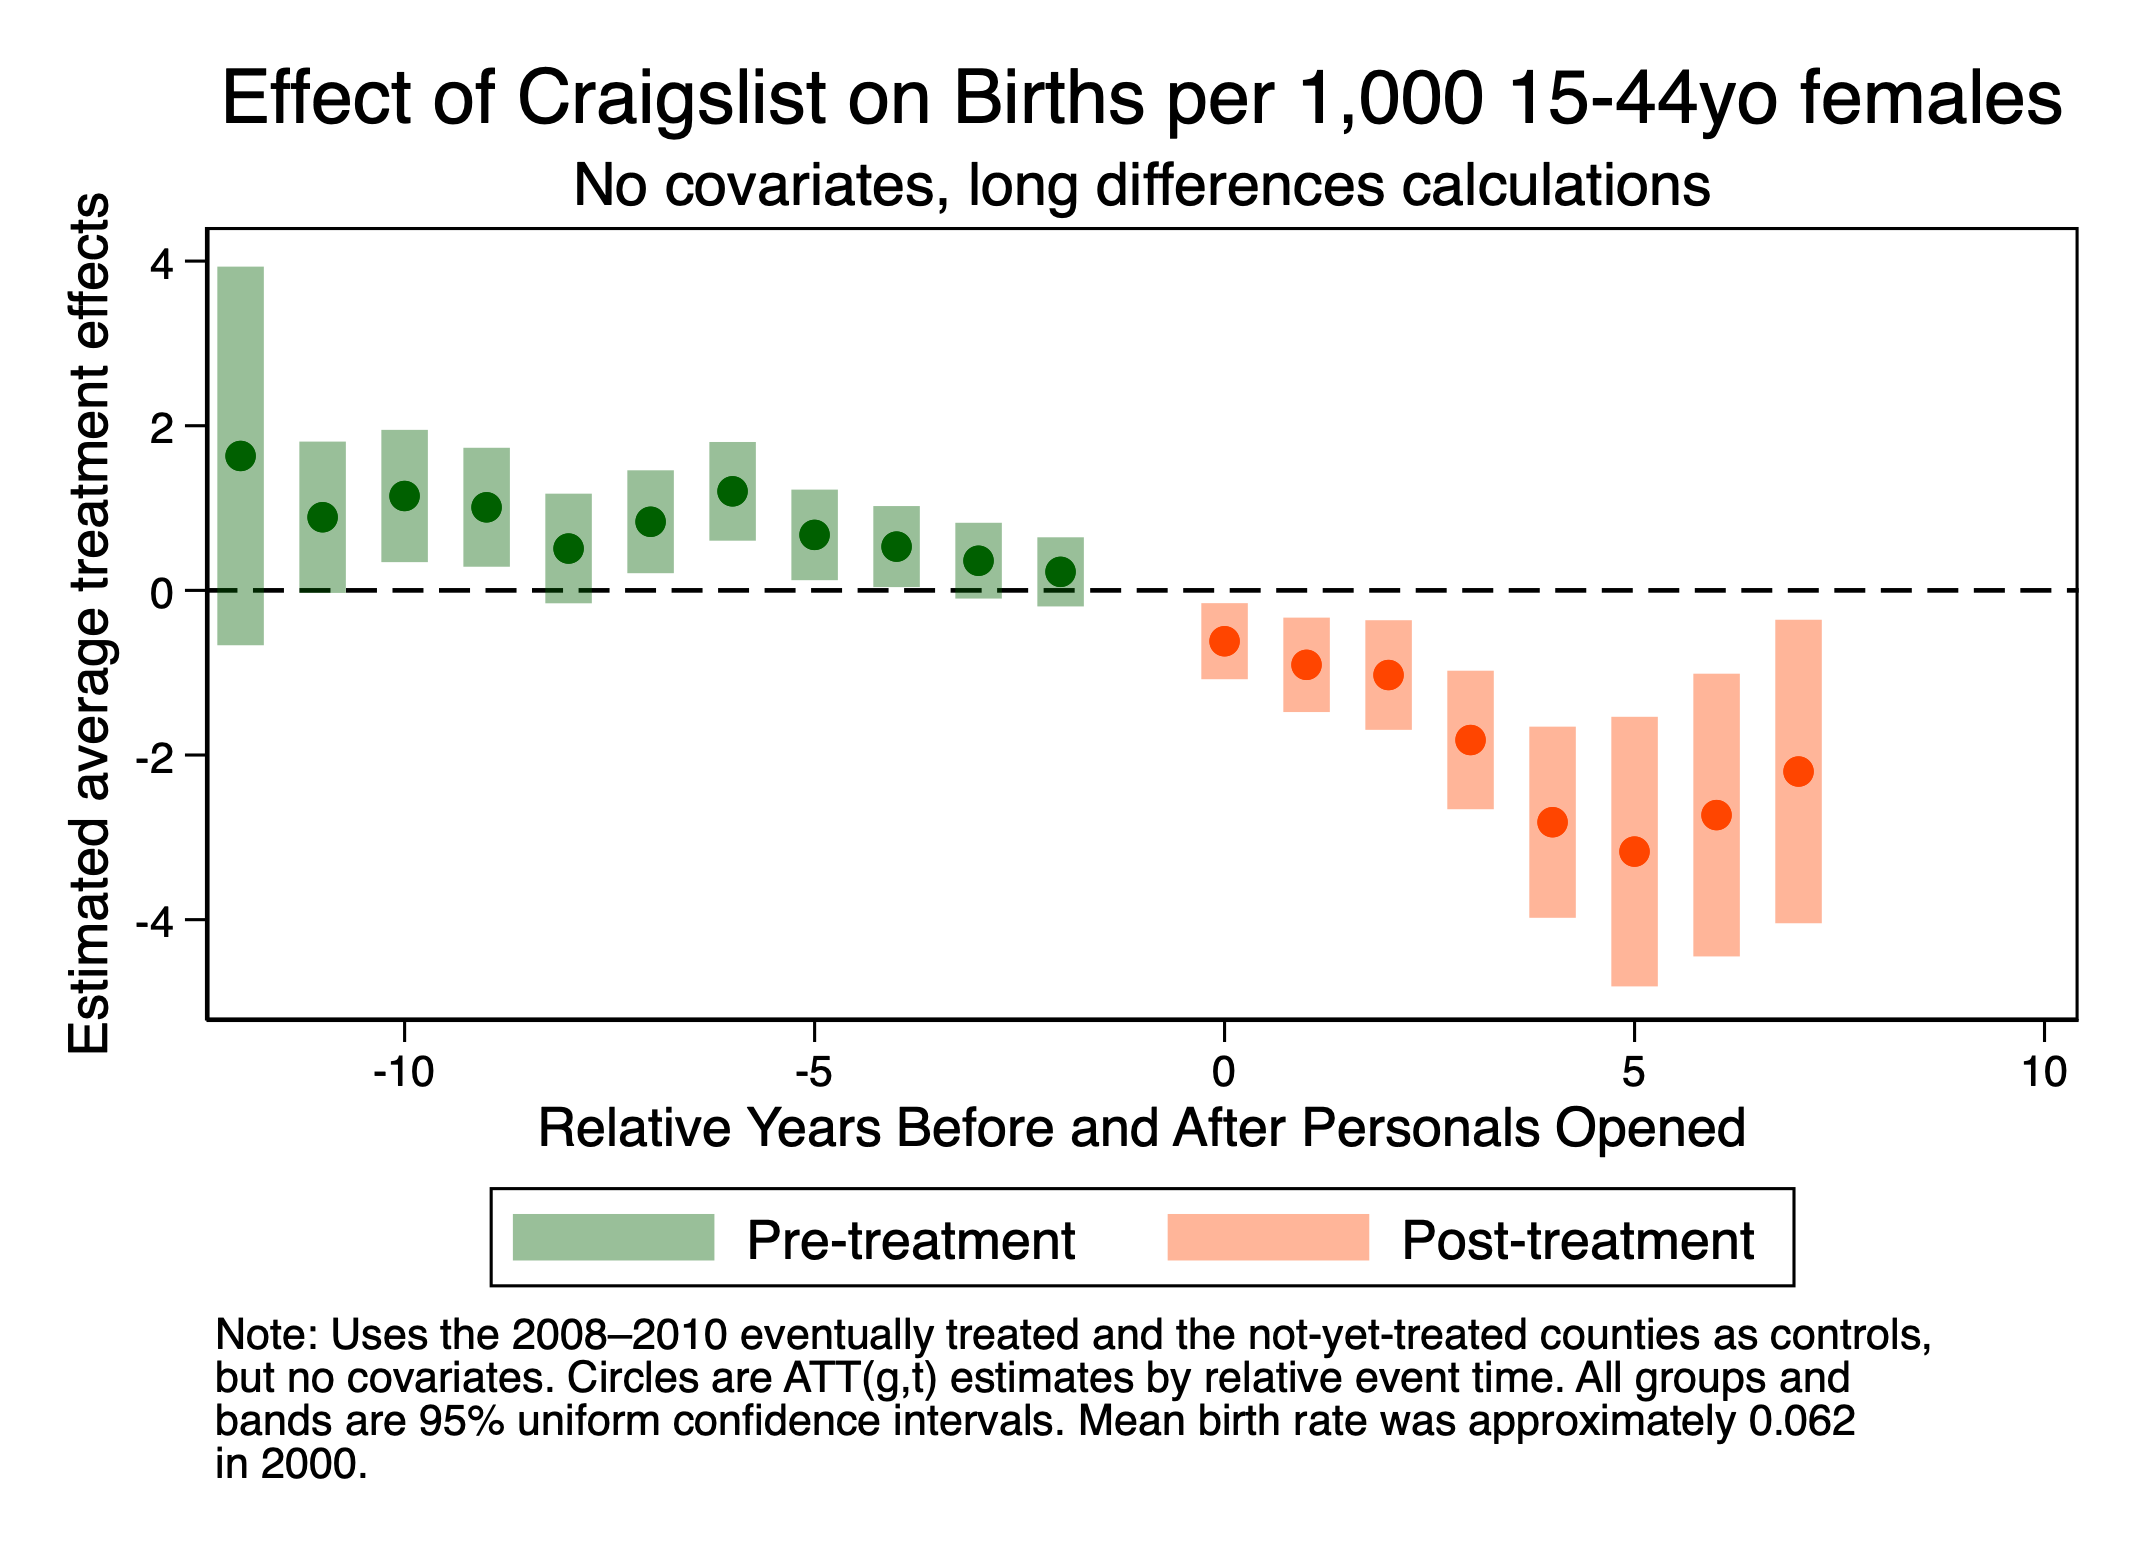
\includegraphics[height=0.85\textheight]{./lecture_includes/es_births_none}
\end{figure}

\end{frame}


\begin{frame}{Trends or No Trends?!}

\begin{figure}[htbp]
    \centering
    \begin{minipage}[b]{0.48\textwidth}
        \centering
    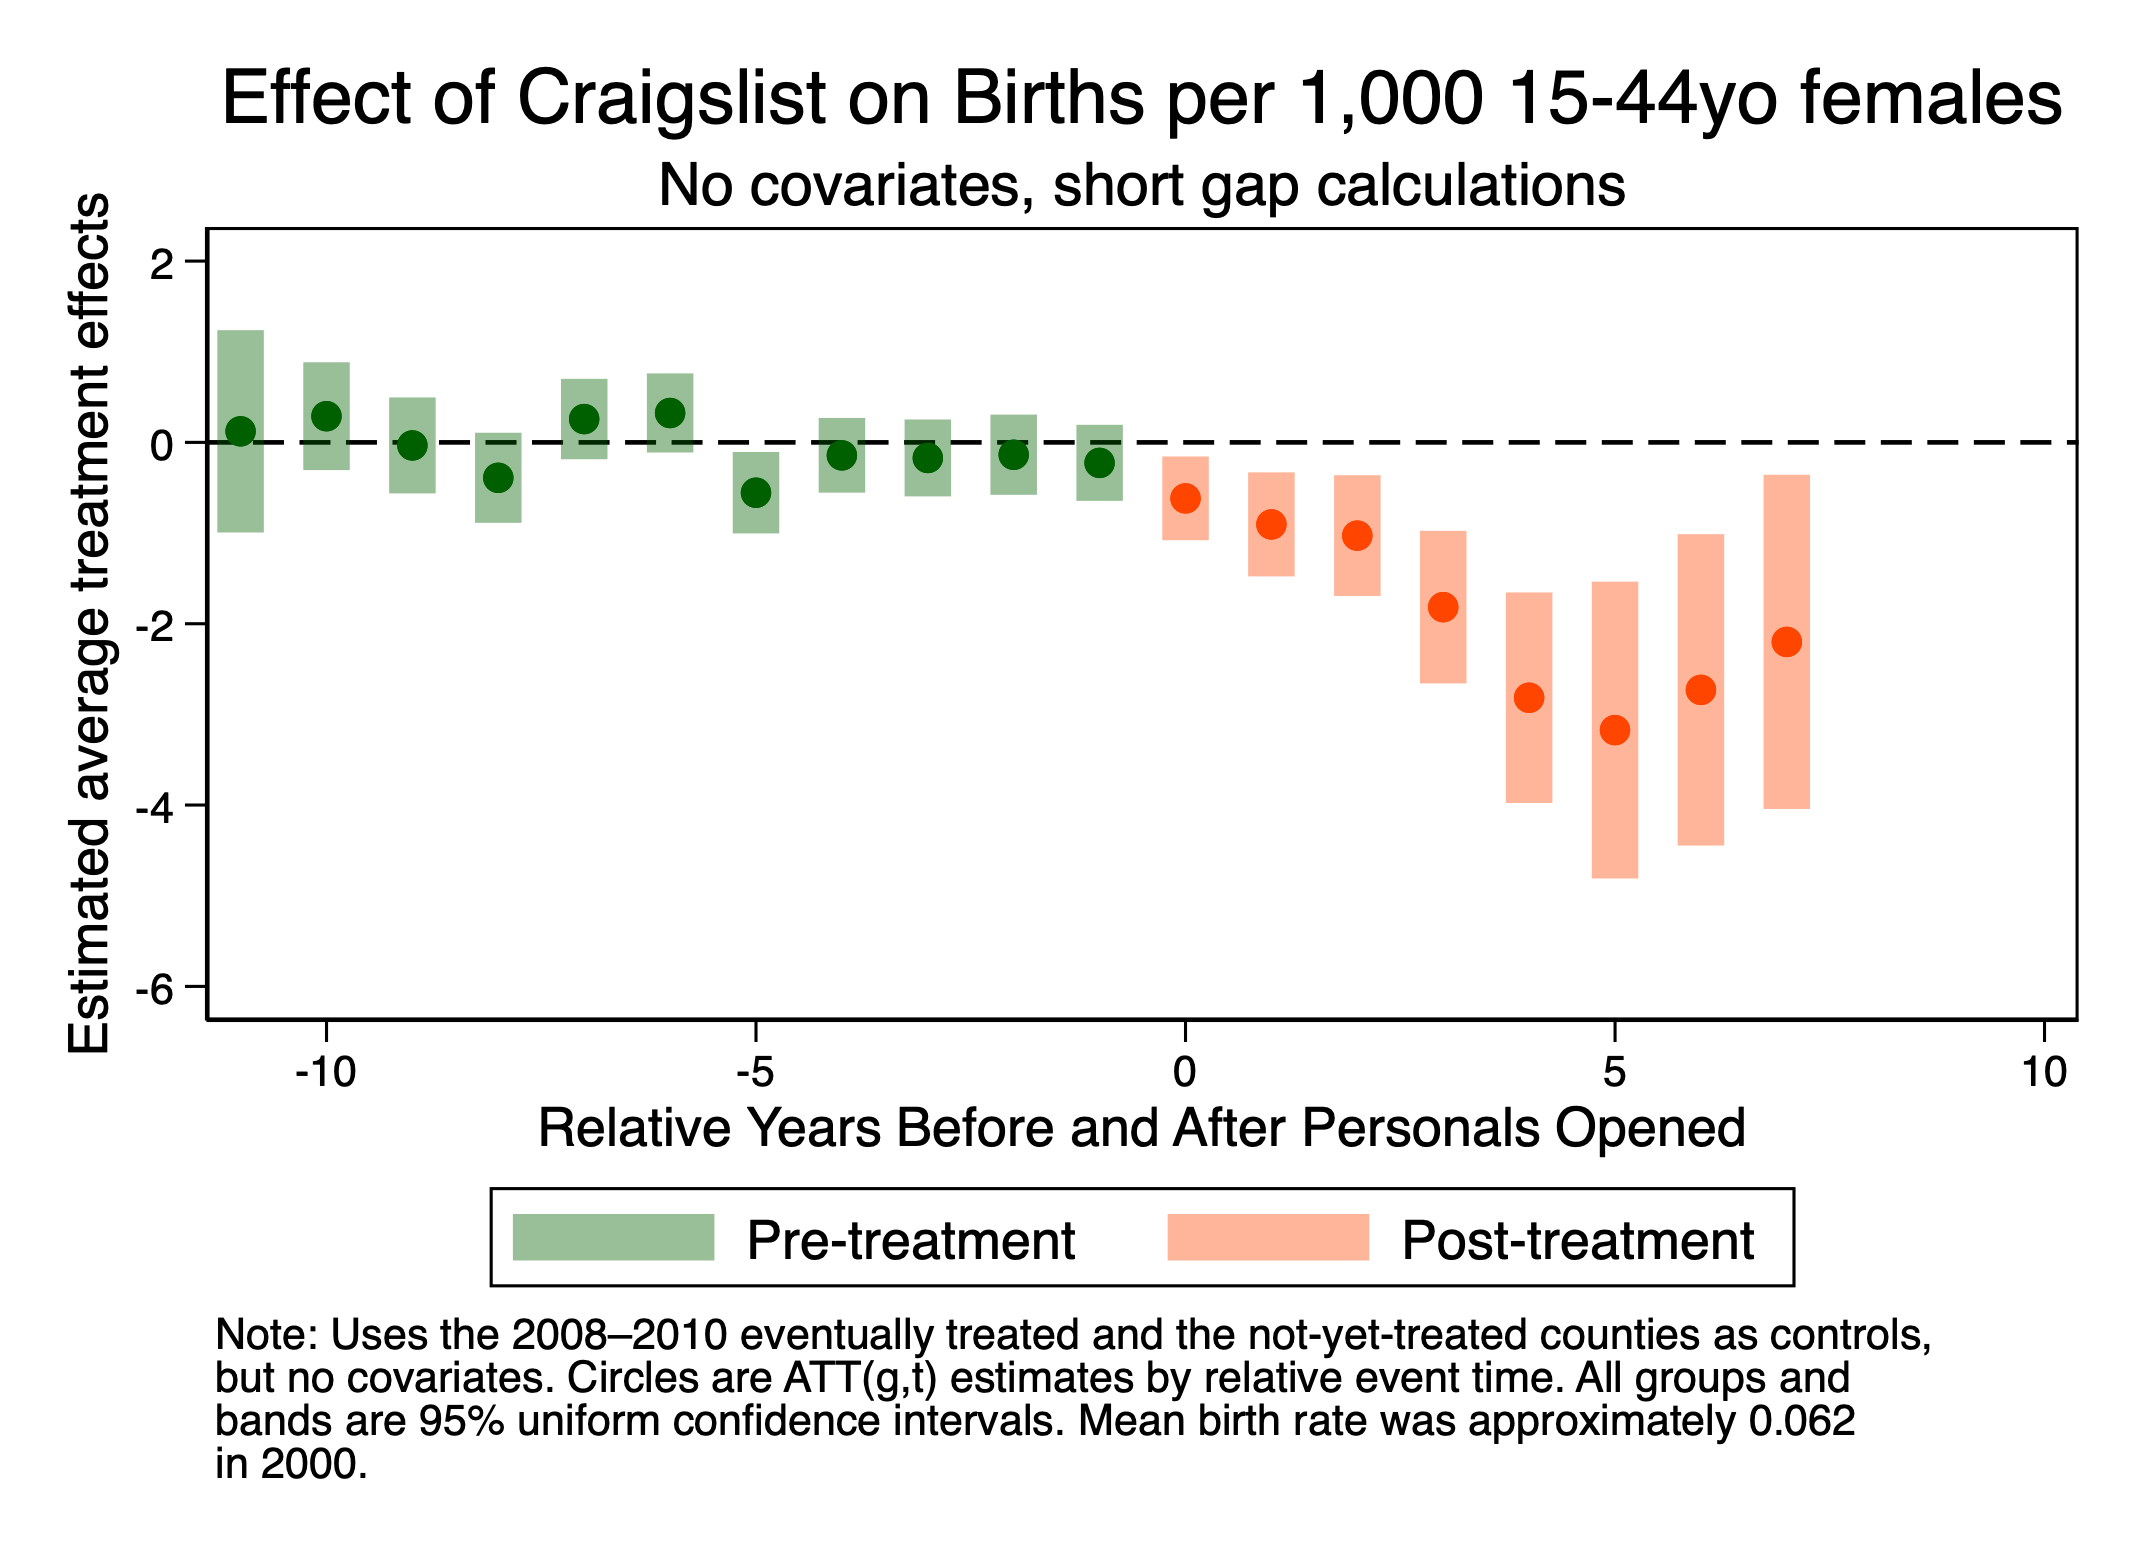
\includegraphics[height=0.45\textheight]{./lecture_includes/es_births_shortnone.png}
        \caption{Short Gap}
    \end{minipage}
    \hfill
    \begin{minipage}[b]{0.48\textwidth}
        \centering
    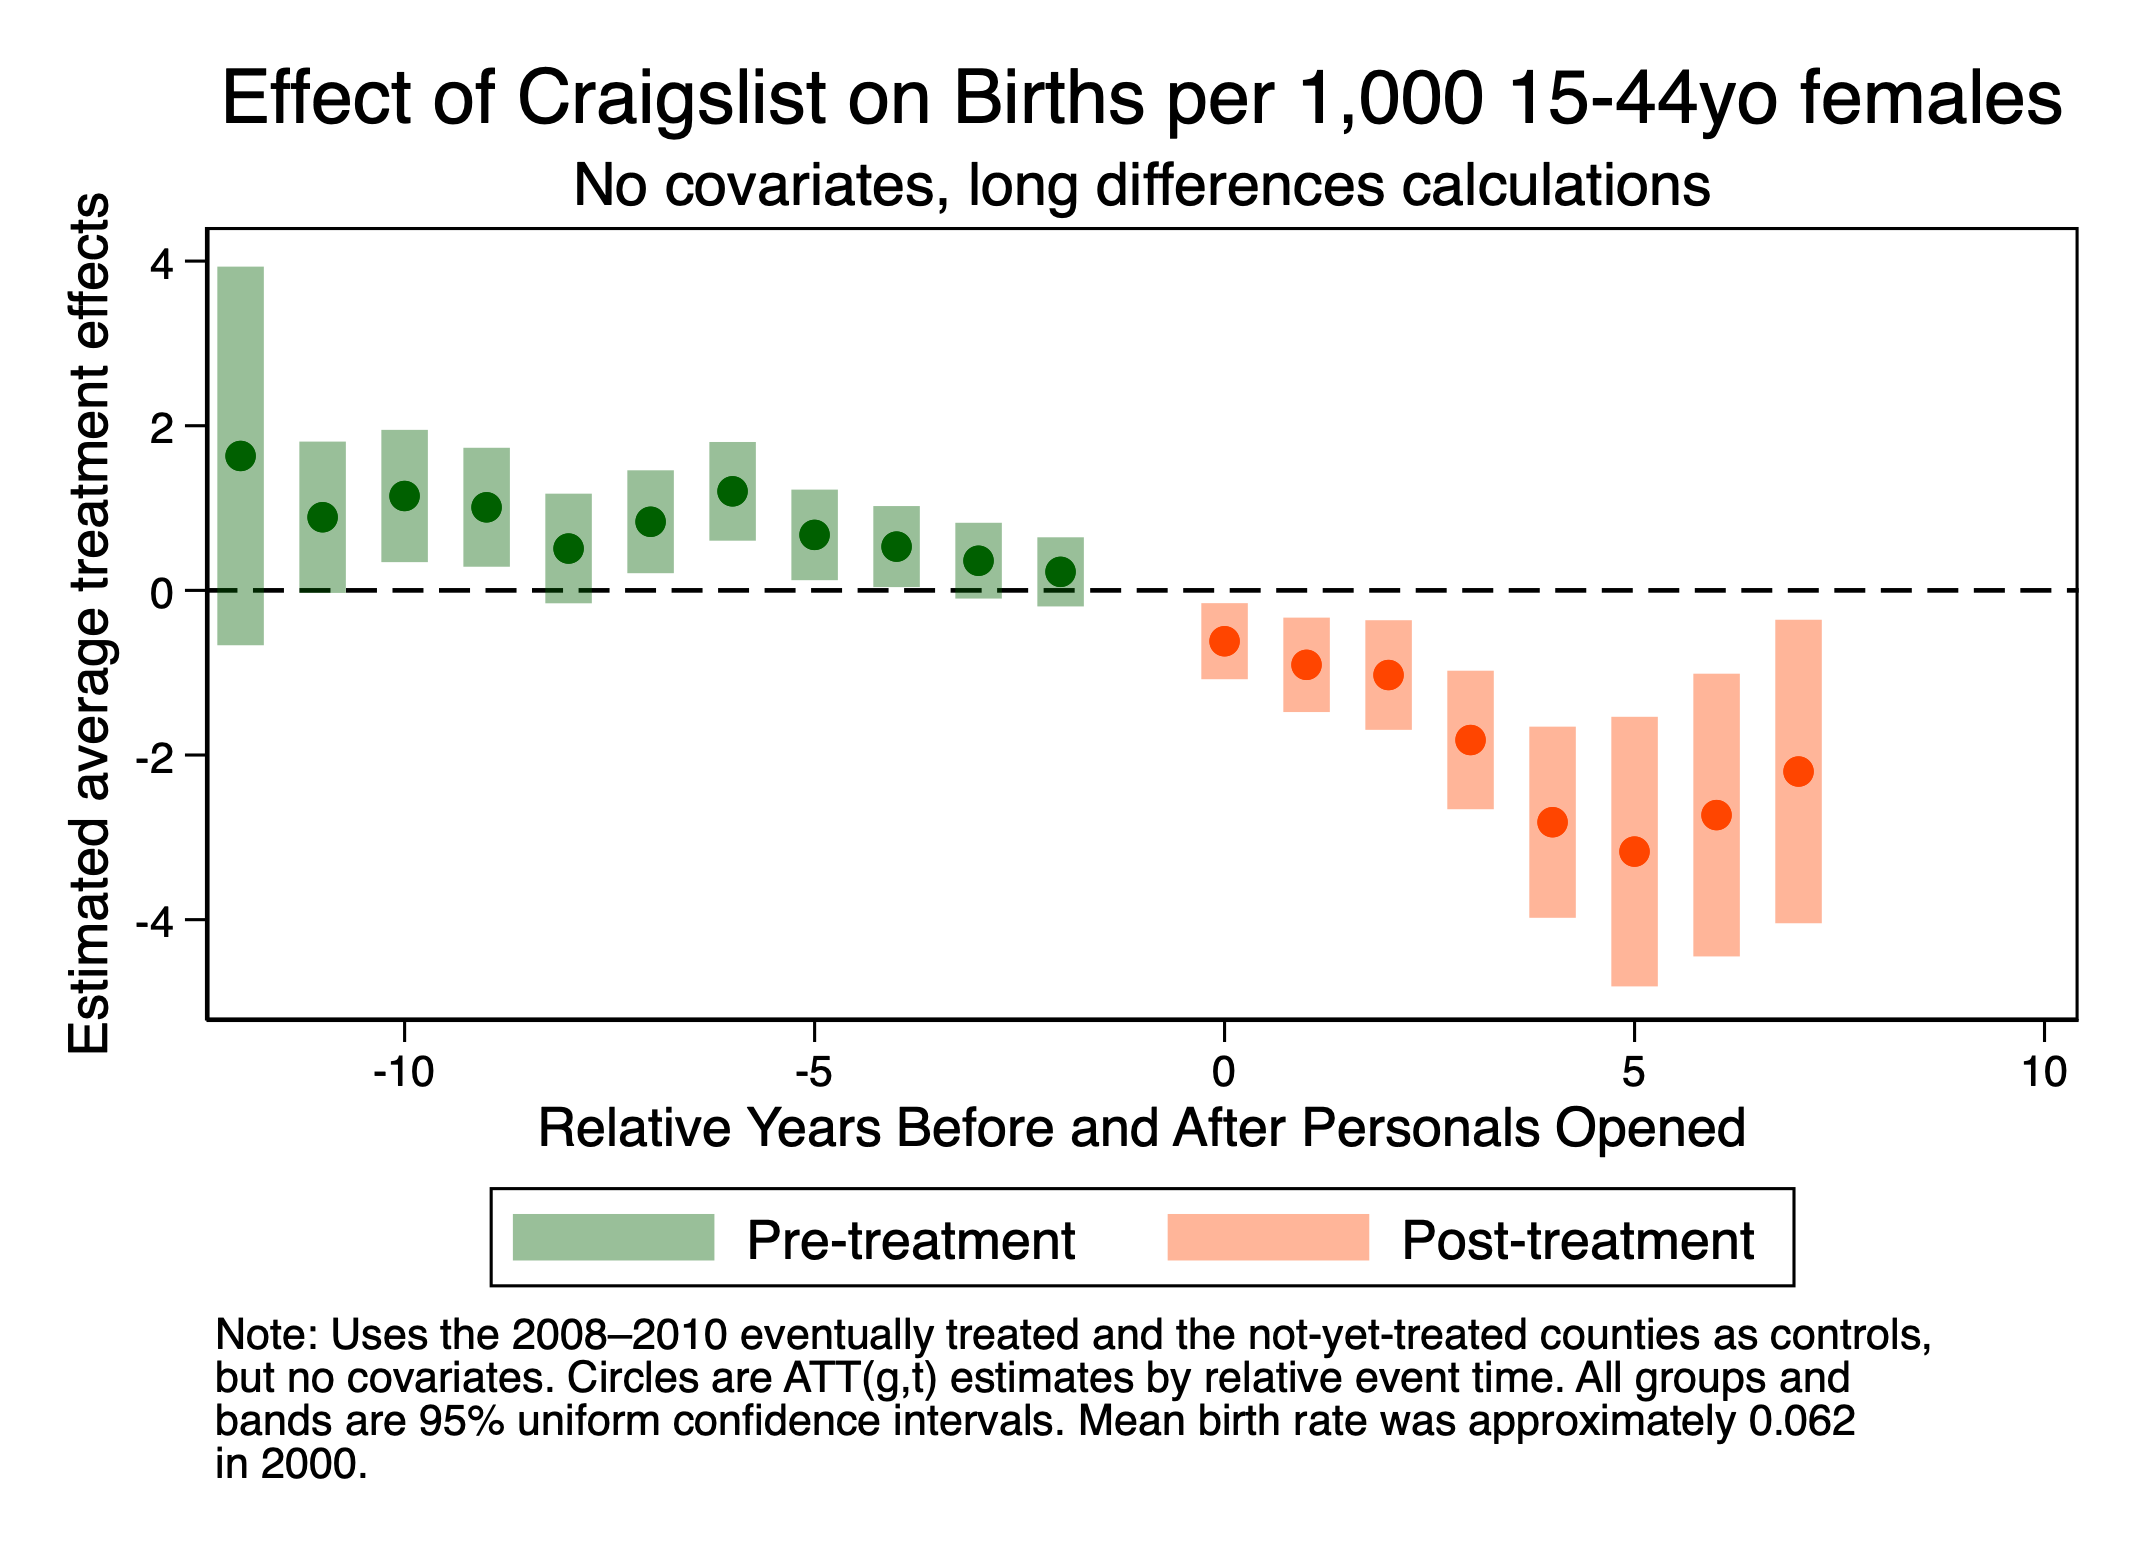
\includegraphics[height=0.45\textheight]{./lecture_includes/es_births_none}
        \caption{Long Difference}
    \end{minipage}
\end{figure}

\end{frame}


\begin{frame}{Scrutinizing that event study}

\begin{itemize}
\item I was so excited when I saw those flat pre-trends until I learned that the default syntax in Stata's \texttt{csdid} calculated short gaps!
\item We had a whole story that online dating caused "permanent dating" until I realized that!! lol
\item But more than that -- was unconditional parallel trends really plausible?  
\item We are assuming the mean change in "untreated birth rates" is the same in our timing cohorts as the comparison cohort, but that assumes a particular "similar control group" and we have no covariates
\end{itemize}
\end{frame}



\begin{frame}{Who got a Craigslist and who didn't?}

\begin{itemize}

\item Craigslist is this: \url{houston.craigslist.org} for Houston, Texas
\item I grew up in a town in Mississippi called Brookhaven with a population of 11,000 and if you search for \url{brookhaven.craigslist.org} it's not there
\item Craigslist targeted \emph{cities} but most of the US counties are \emph{rural}
\end{itemize}

\end{frame}



\begin{frame}{Is Unconditional parallel trends plausible?}

\begin{itemize}
\item But my coauthors are demographers who focus a lot on maternal health and children, plus they're labor economists and they urban counties and rural counties differ:
	\begin{itemize}
	\item Cities have more college educated women, delayed childbearing, lower marriage rates, different racial composition, more access to female healthcare resources
	\item Rural towns have lower educated women, earlier age at first birth, higher marriage rates, more homogenous, worse healthcare access
	\end{itemize}
\item If Craigslist counties are more urban, then our treatment and control are imbalance on covariates that cause trends in $Y^0$
\item Let's look at mean female population and urban measures by timing cohort
\end{itemize}

\end{frame}


\begin{frame}{Female population by timing cohort}

\begin{figure}
    \centering
    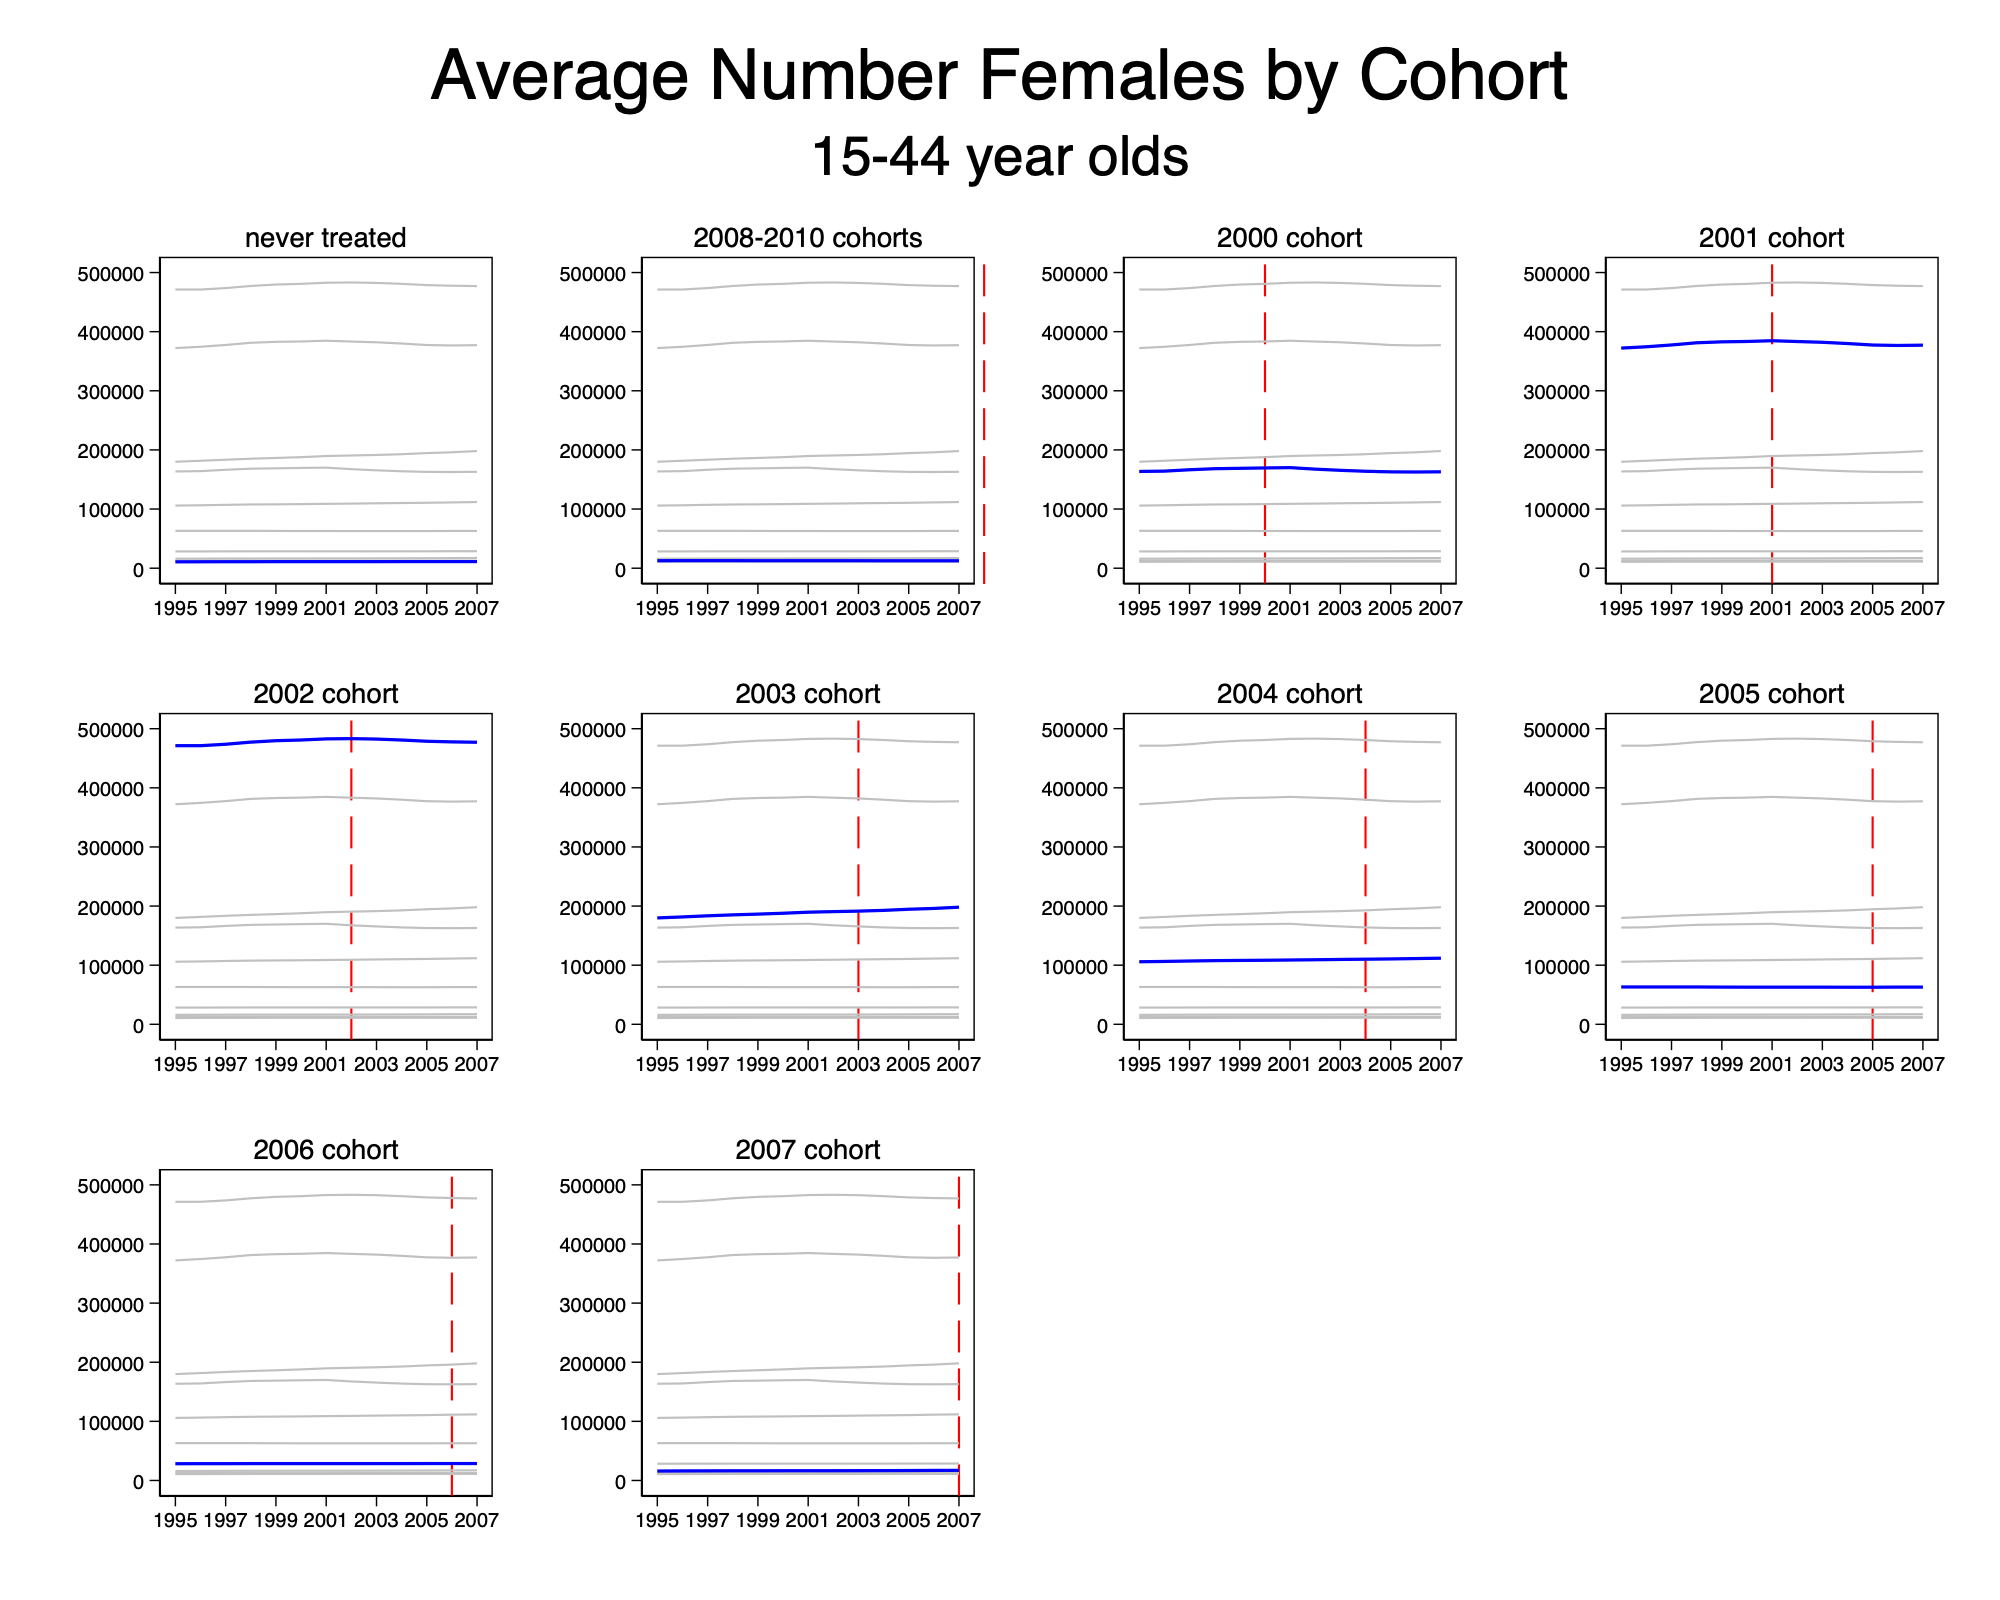
\includegraphics[height=0.85\textheight]{./lecture_includes/pretty_fempop}
\end{figure}

\end{frame}


\begin{frame}{Urban and rural counties by timing cohort}

\begin{figure}
    \centering
    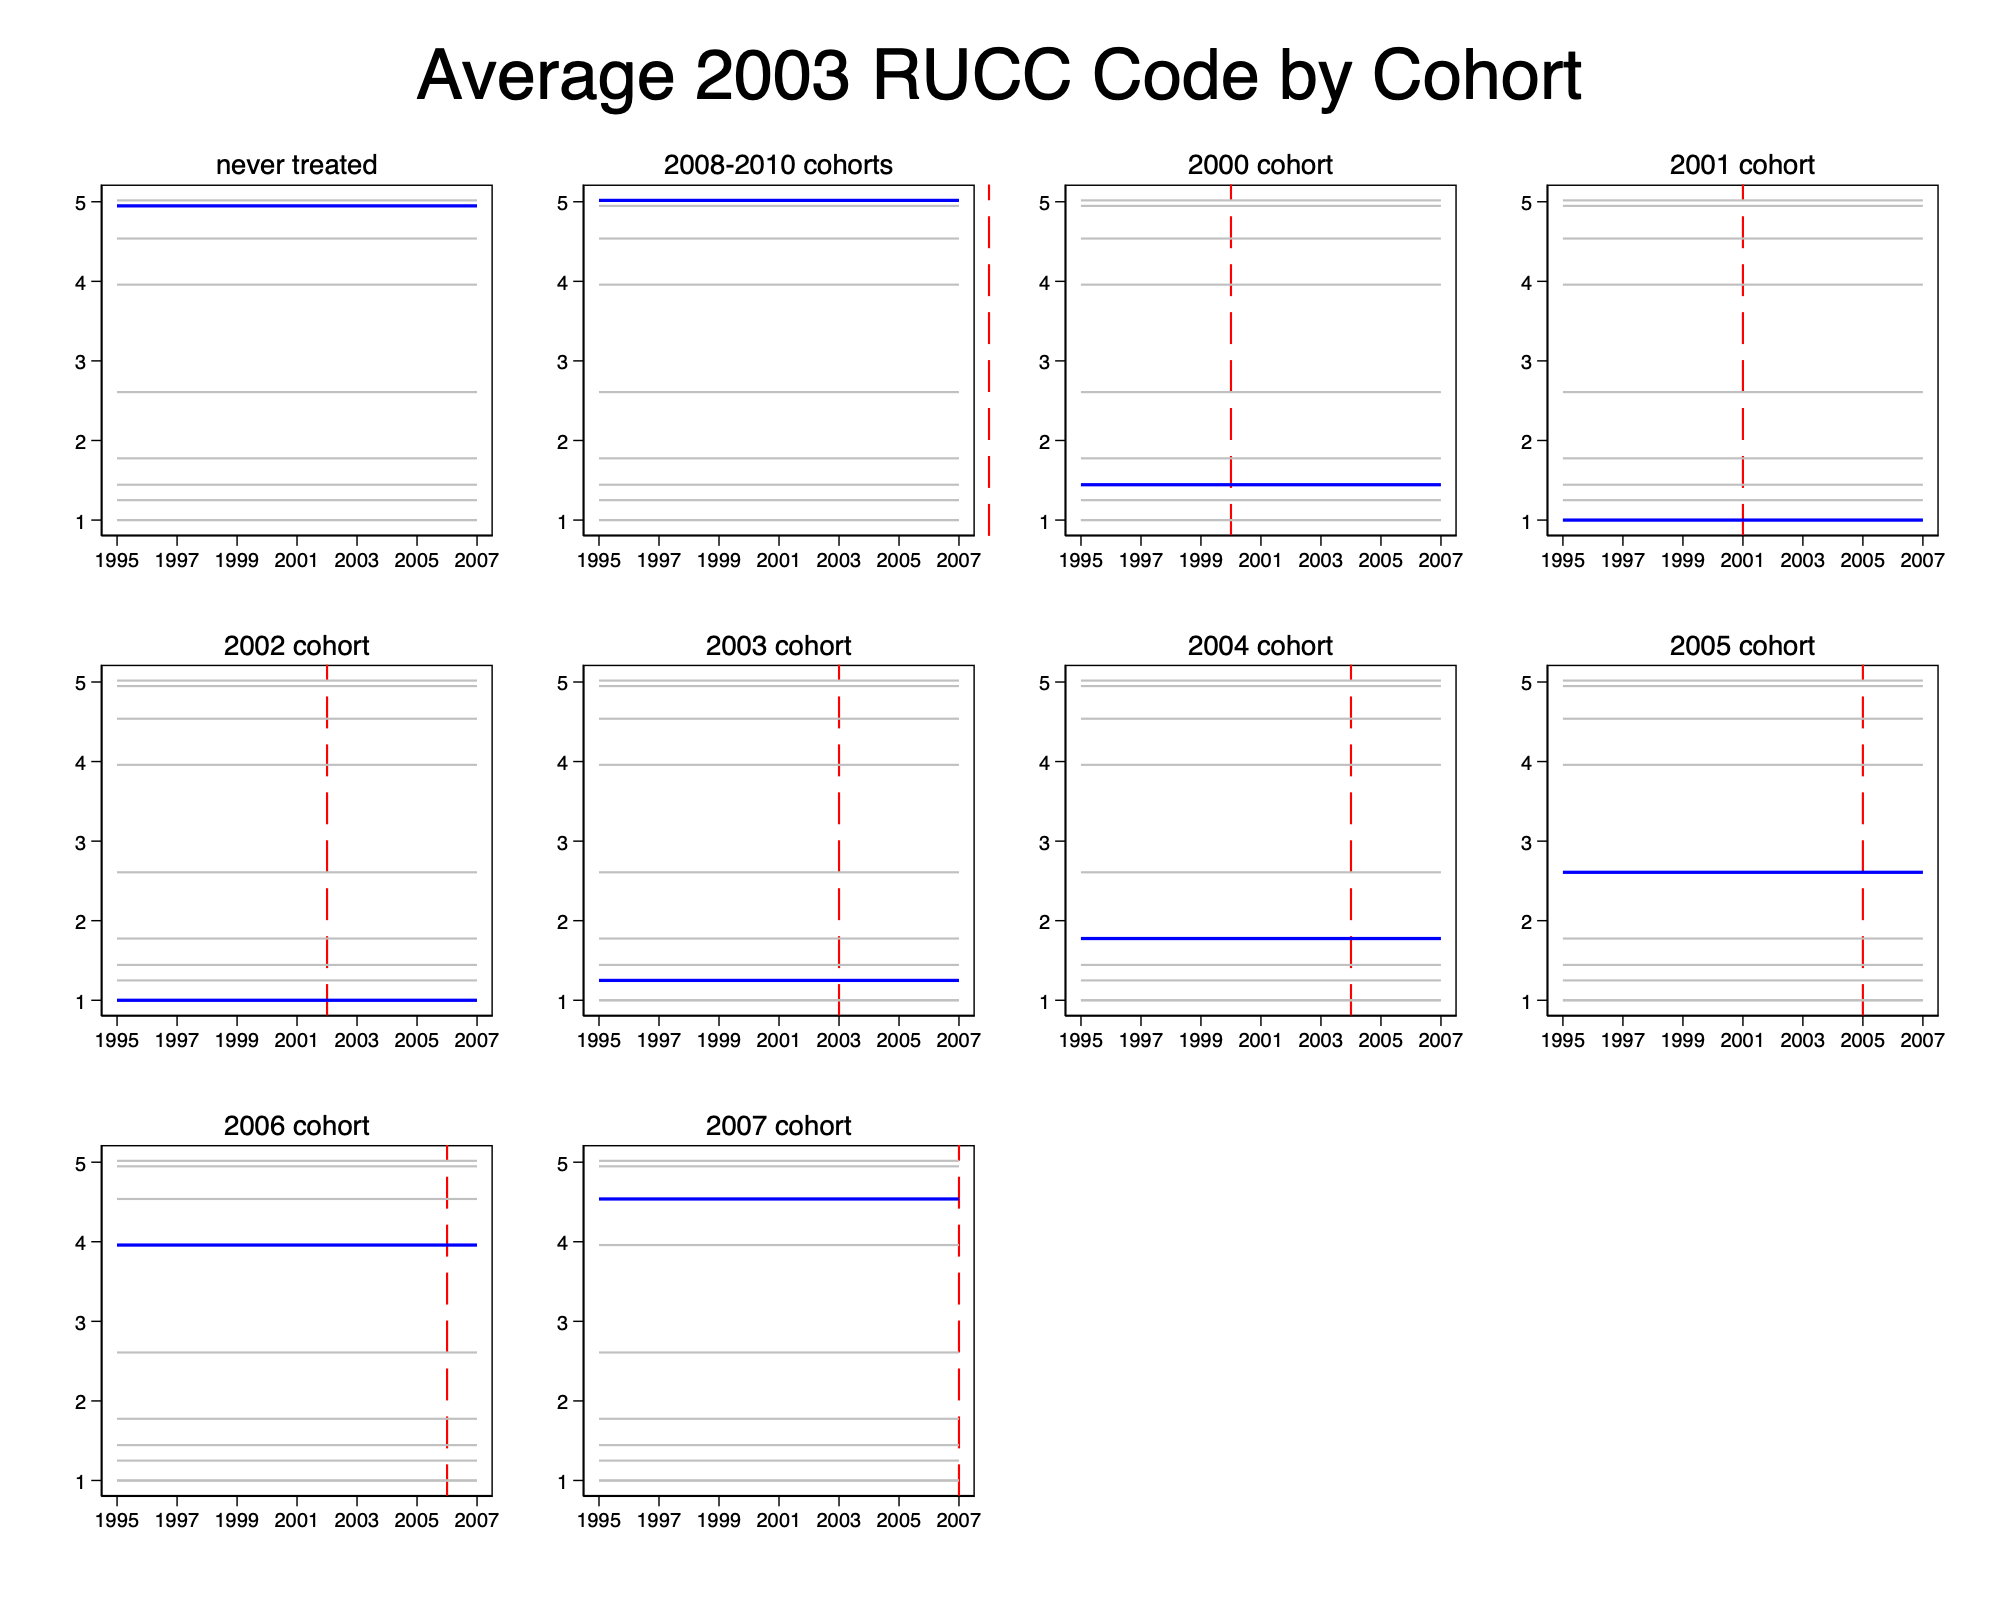
\includegraphics[height=0.85\textheight]{./lecture_includes/pretty_RUCC}
\end{figure}

\end{frame}



\begin{frame}{Control for 9-digit urban code}

\begin{itemize}

\item So we decided -- and I still remember this day -- to just include one variable
\item 9-digit RUCC code measuring "how urban is the county?"
	\begin{itemize}
	\item RUCC code of 1: VERY URBAN (e.g., San Francisco)
	\item RUCC code of 9: VERY RURAL (e.g., Brookhaven)
	\end{itemize}
\item Effectively, what is happening when we do this, it is as though we are estimating CS for 1s, 2s, 3s, and so on
\item Our control group is so large they have \emph{every RUCC code}
\item So, we estimate CS with 8 RUCC dummies (more dramatic if I show it to you)
\end{itemize}

\end{frame}




\begin{frame}{Long Differences, with and without RUCC dummies}

\begin{figure}
    \centering
    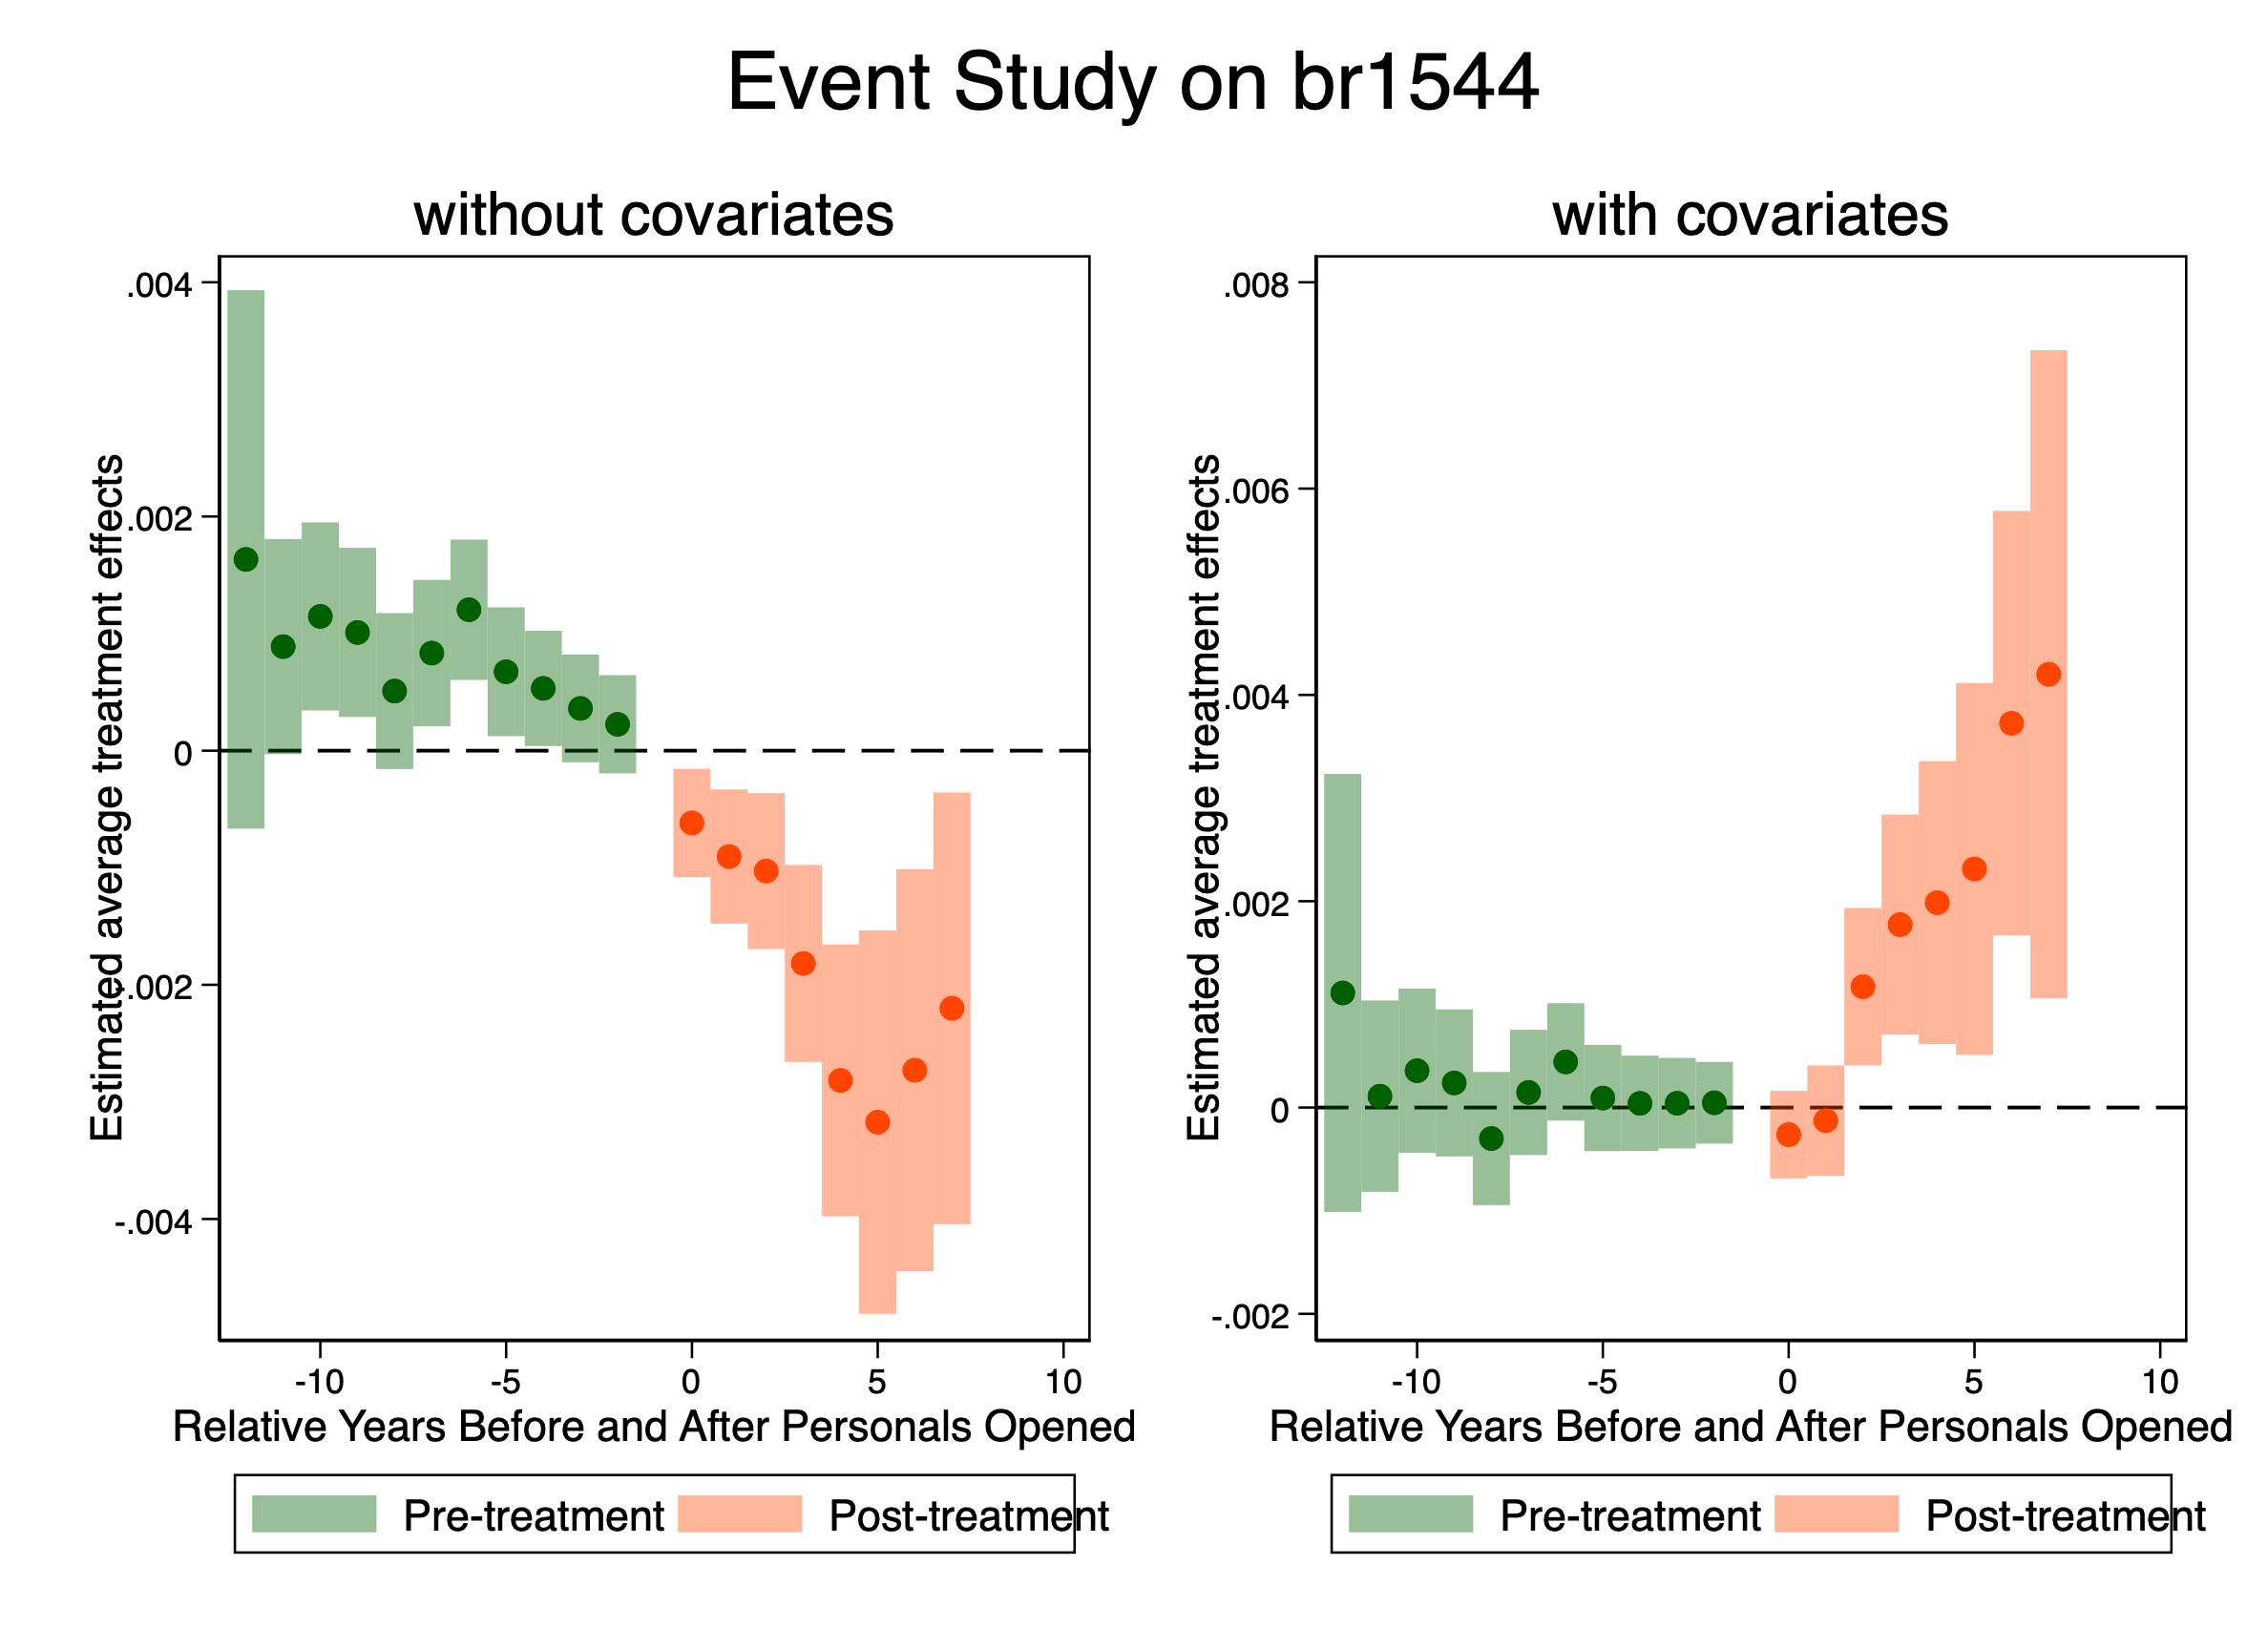
\includegraphics[height=0.85\textheight]{./lecture_includes/es_br1544_combined.png}
\end{figure}

\end{frame}

\begin{frame}{Now put yourself in my shoes!}

\begin{figure}[htbp]
    \centering
    \begin{minipage}[b]{0.48\textwidth}
        \centering
    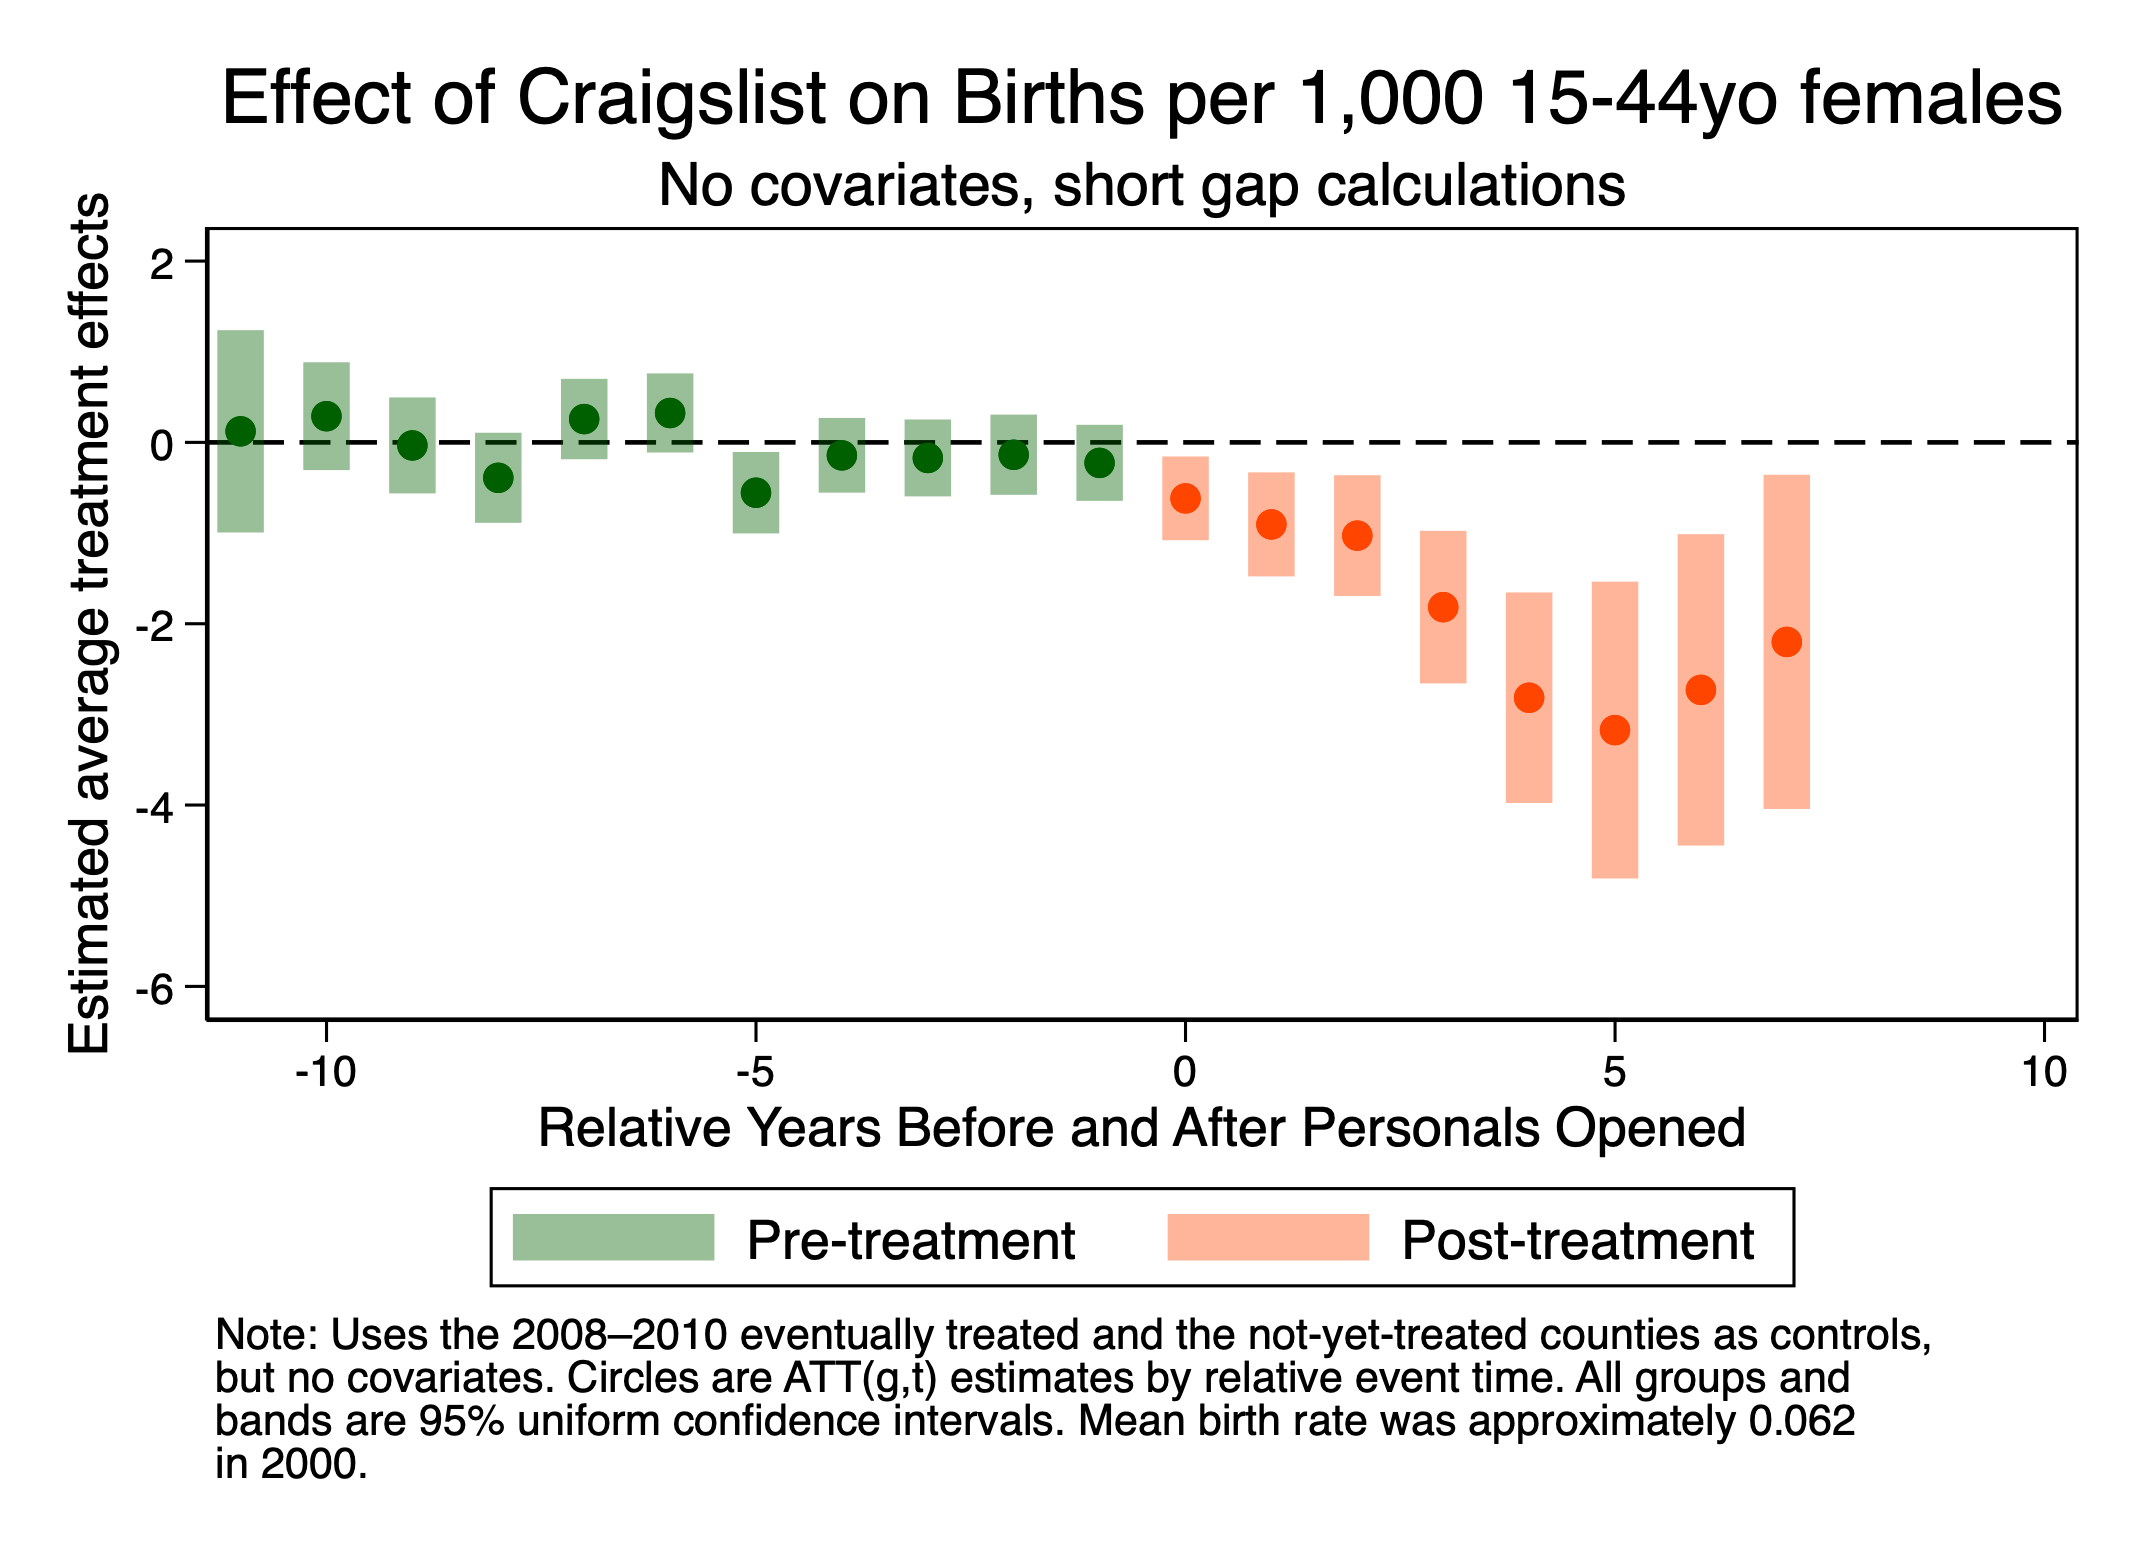
\includegraphics[height=0.45\textheight]{./lecture_includes/es_births_shortnone}
        \caption{Short Gap, no covariates}
    \end{minipage}
    \hfill
    \begin{minipage}[b]{0.48\textwidth}
        \centering
    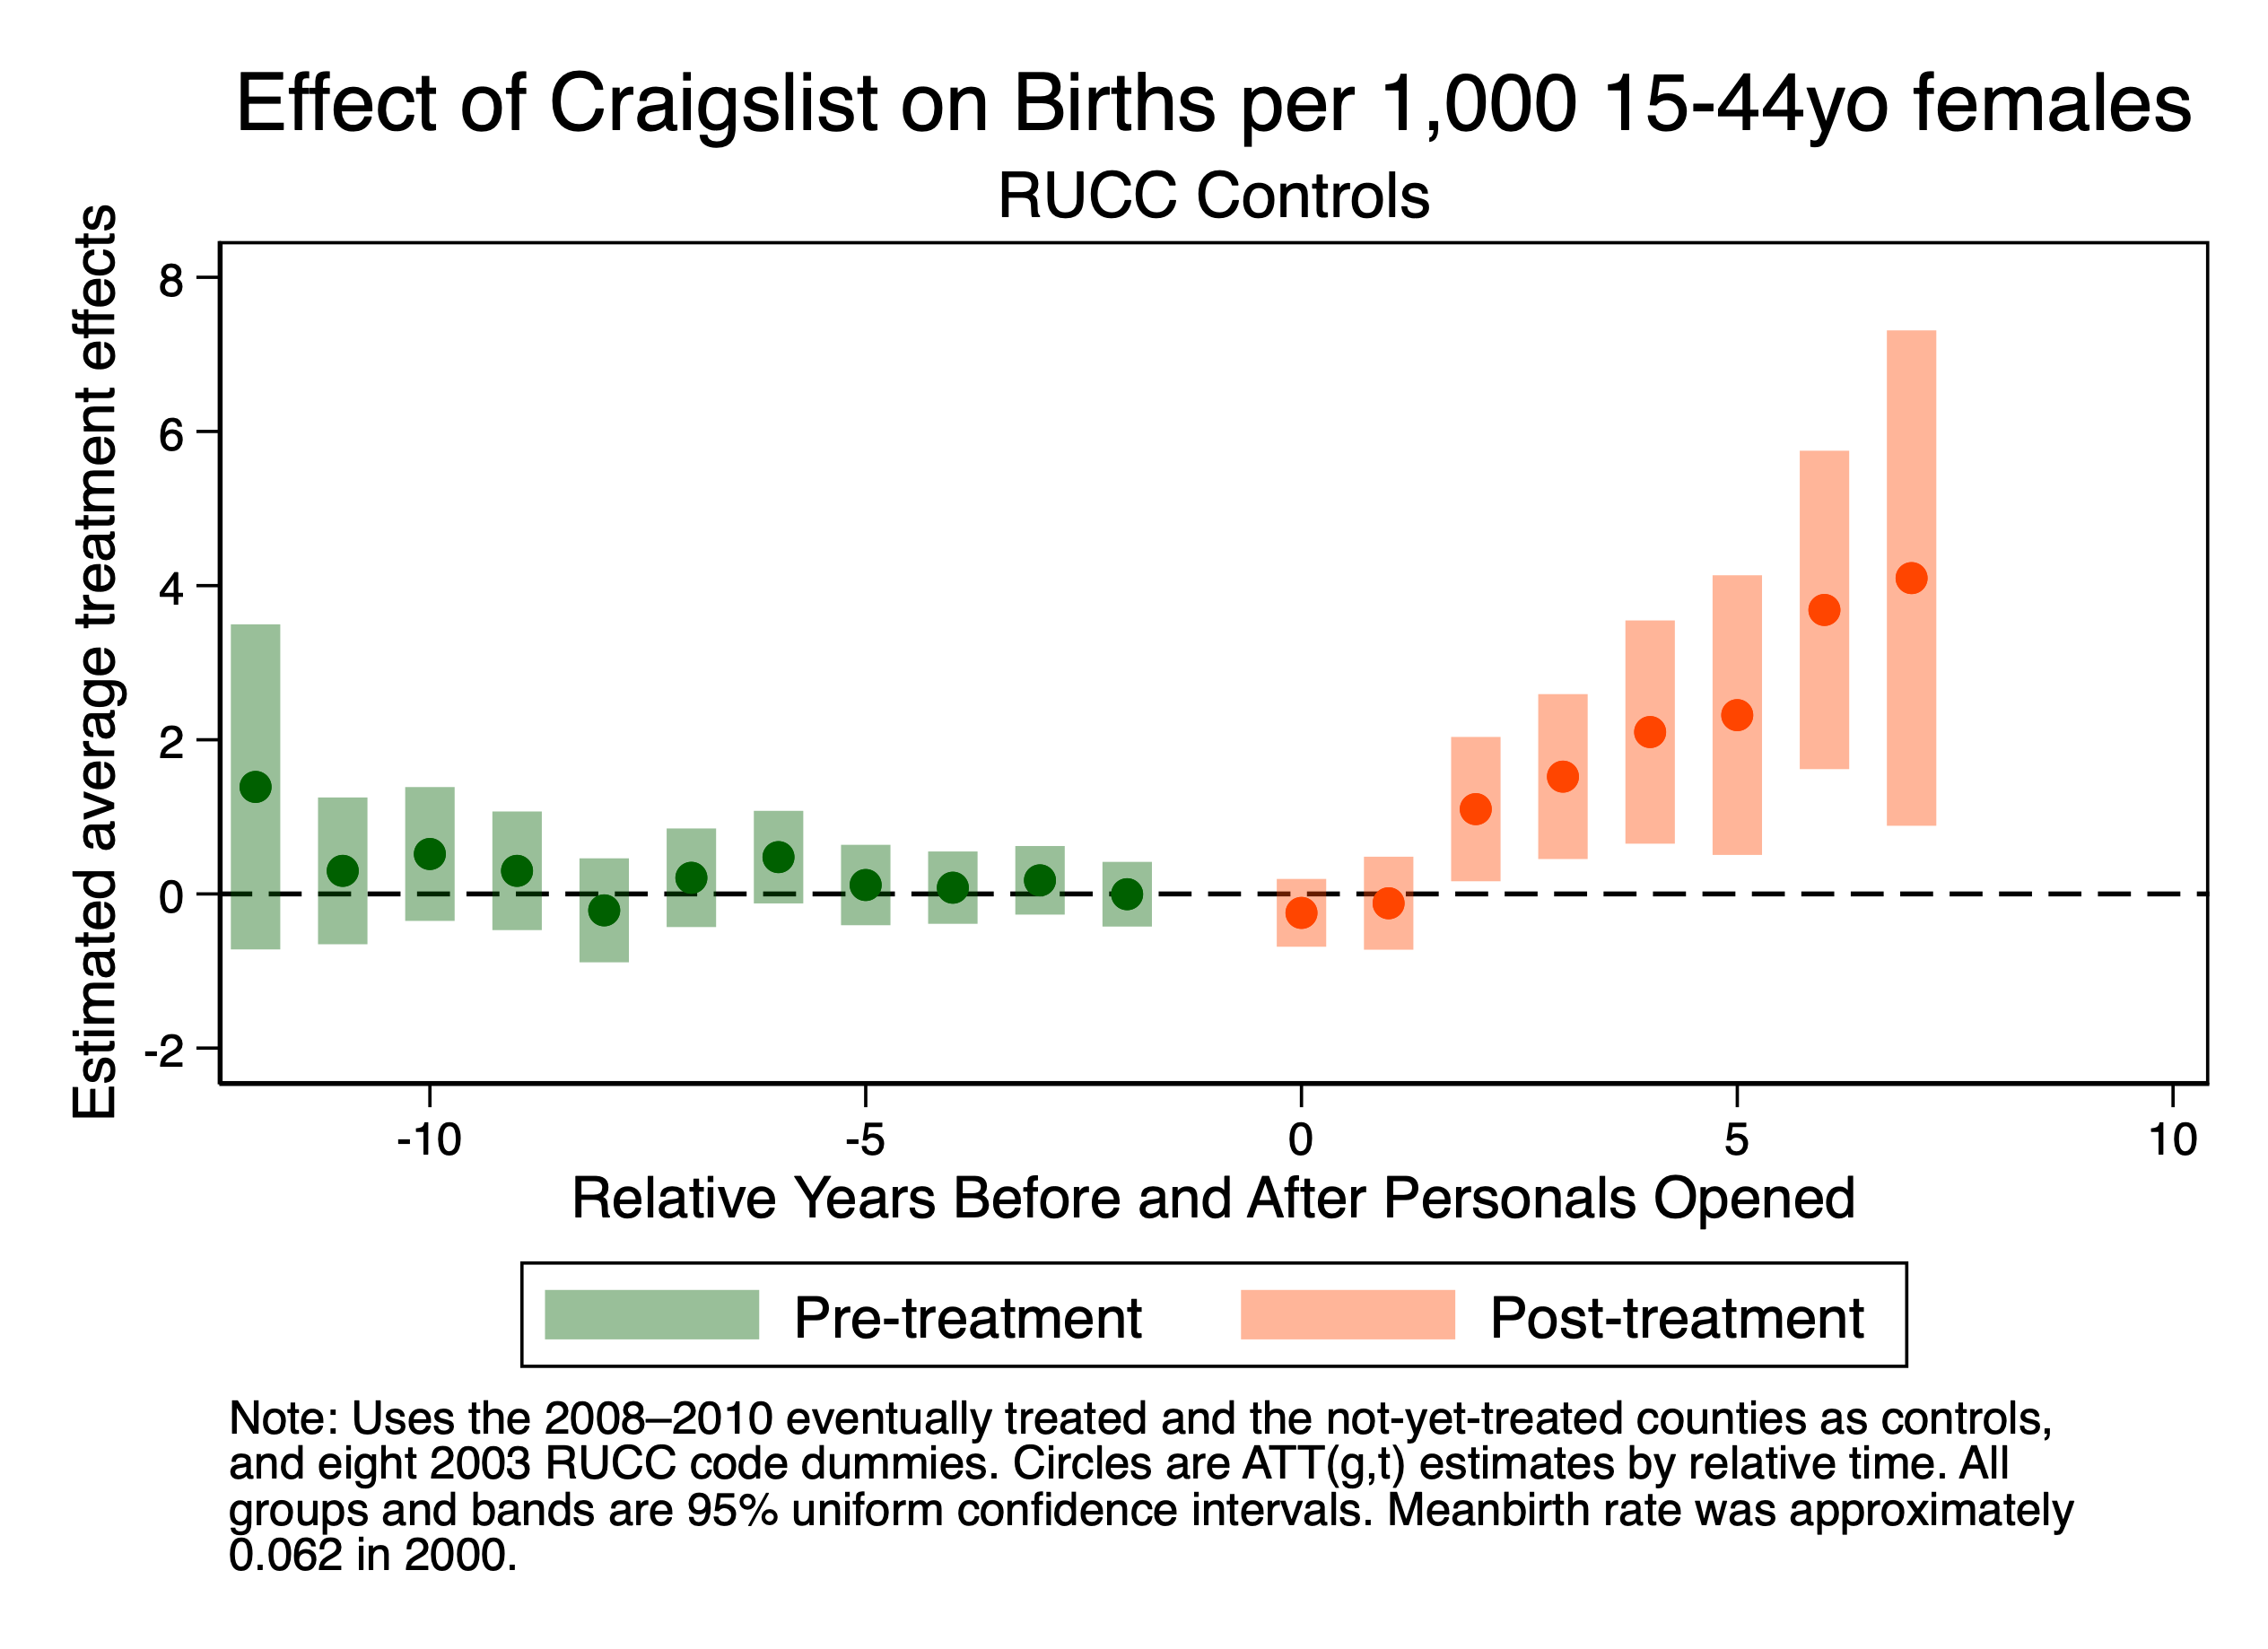
\includegraphics[height=0.45\textheight]{./lecture_includes/es_births_RUCC.png}
        \caption{Long Difference, 8 RUCC dummies}
    \end{minipage}
\end{figure}

\end{frame}

\begin{frame}{Any more covariates?}

\begin{itemize}

\item So then we started asking ourselves -- is urban enough?  And how will we decide?
\item We decided we urban dummies captured a lot of things, but we wanted more, but what and how will we decide so limit specification searching
\item We decided to LASSO on $\Delta Birth\_rates$ using only the pretreatment periods because $\Delta Y_{t-\tau} = \Delta Y^0_{t-\tau}$ then 

\end{itemize}

\end{frame}

\begin{frame}{Specific LASSO steps}

\begin{enumerate}
\item Regress birth rates on state-year interactions for 1995-1999 (pre-treatment)
\item Took first difference per county for residuals
\item LASSO regression of first difference residuals (county-level)
\item Cross validation
\end{enumerate}

LASSO selected male to female sex ratio, per capita income, and unemployment rates (out of 11 covariates)

\end{frame}

\begin{frame}{CS estimator with 8 RUCC codes, sex ratio, per capita income and unemployment rate}

\begin{figure}
    \centering
    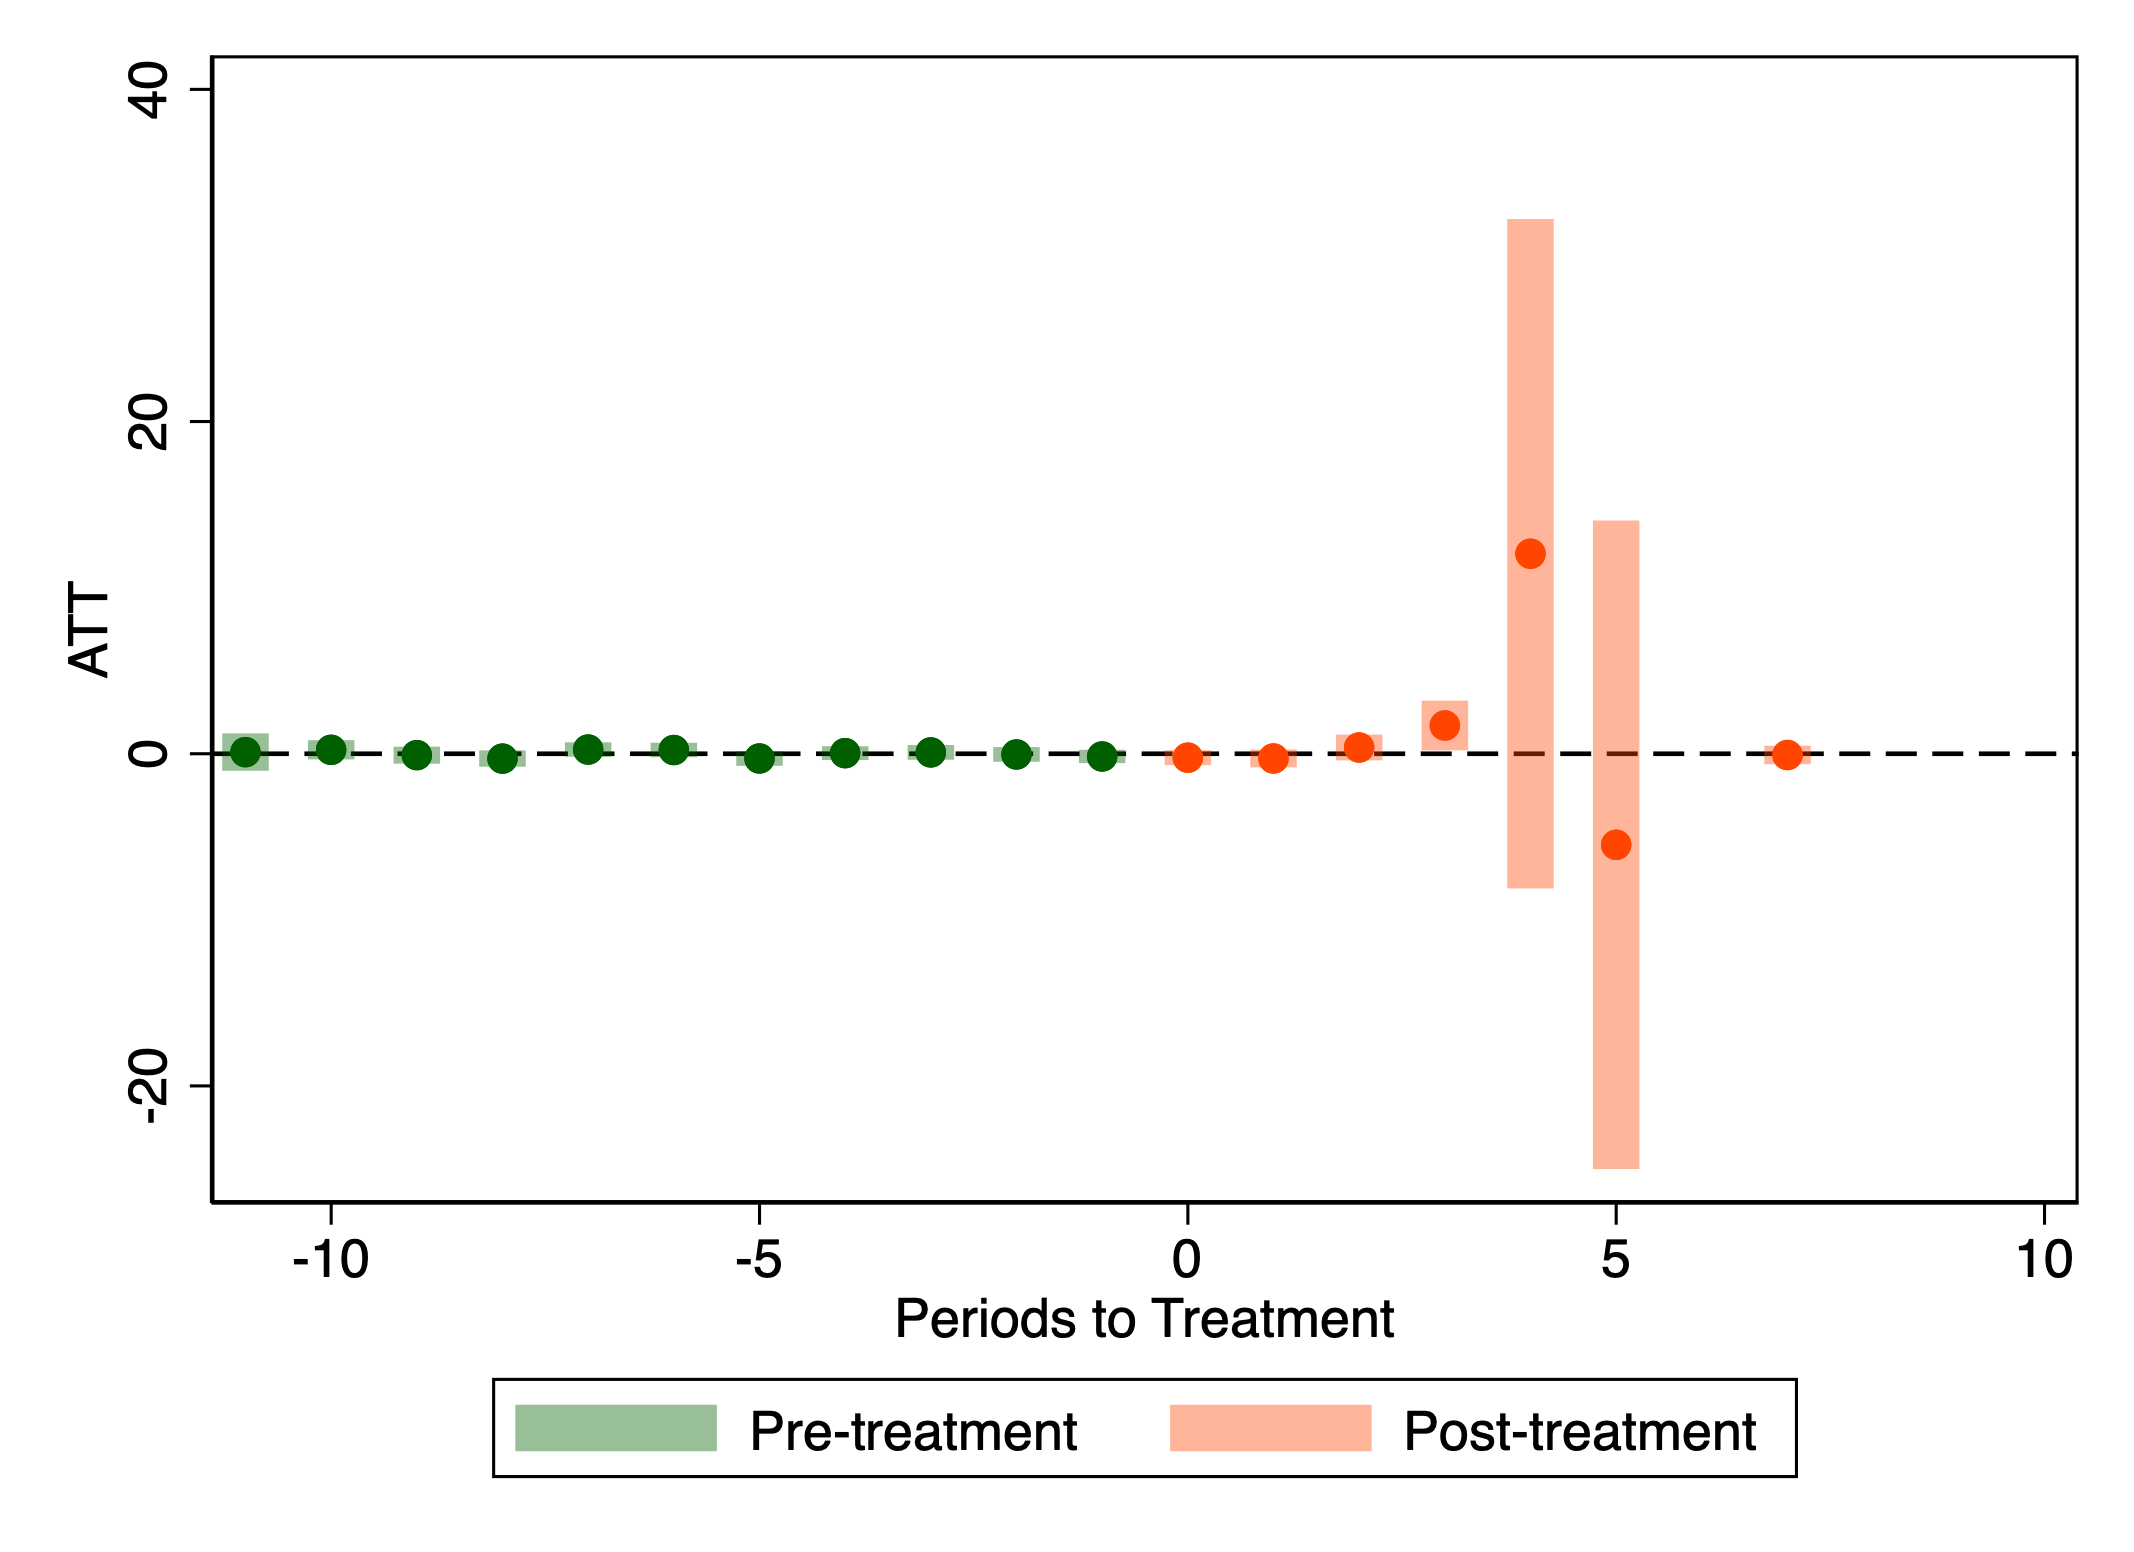
\includegraphics[height=0.85\textheight]{./lecture_includes/lasso_br1544}
\end{figure}

\end{frame}

\begin{frame}
\frametitle{Yikes!}

\begin{itemize}
\item What's going on?  Overlap problems
\item We are creating "separation" caused by curse of dimensionality
\item All of the propensity scores are ending up not overlapping
\item So we had to discretize the covariates into quantiles
\end{itemize}

\end{frame}


\begin{frame}{CS estimator with 8 RUCC codes, sex ratio, per capita income and unemployment rate quantiles}

\begin{figure}
    \centering
    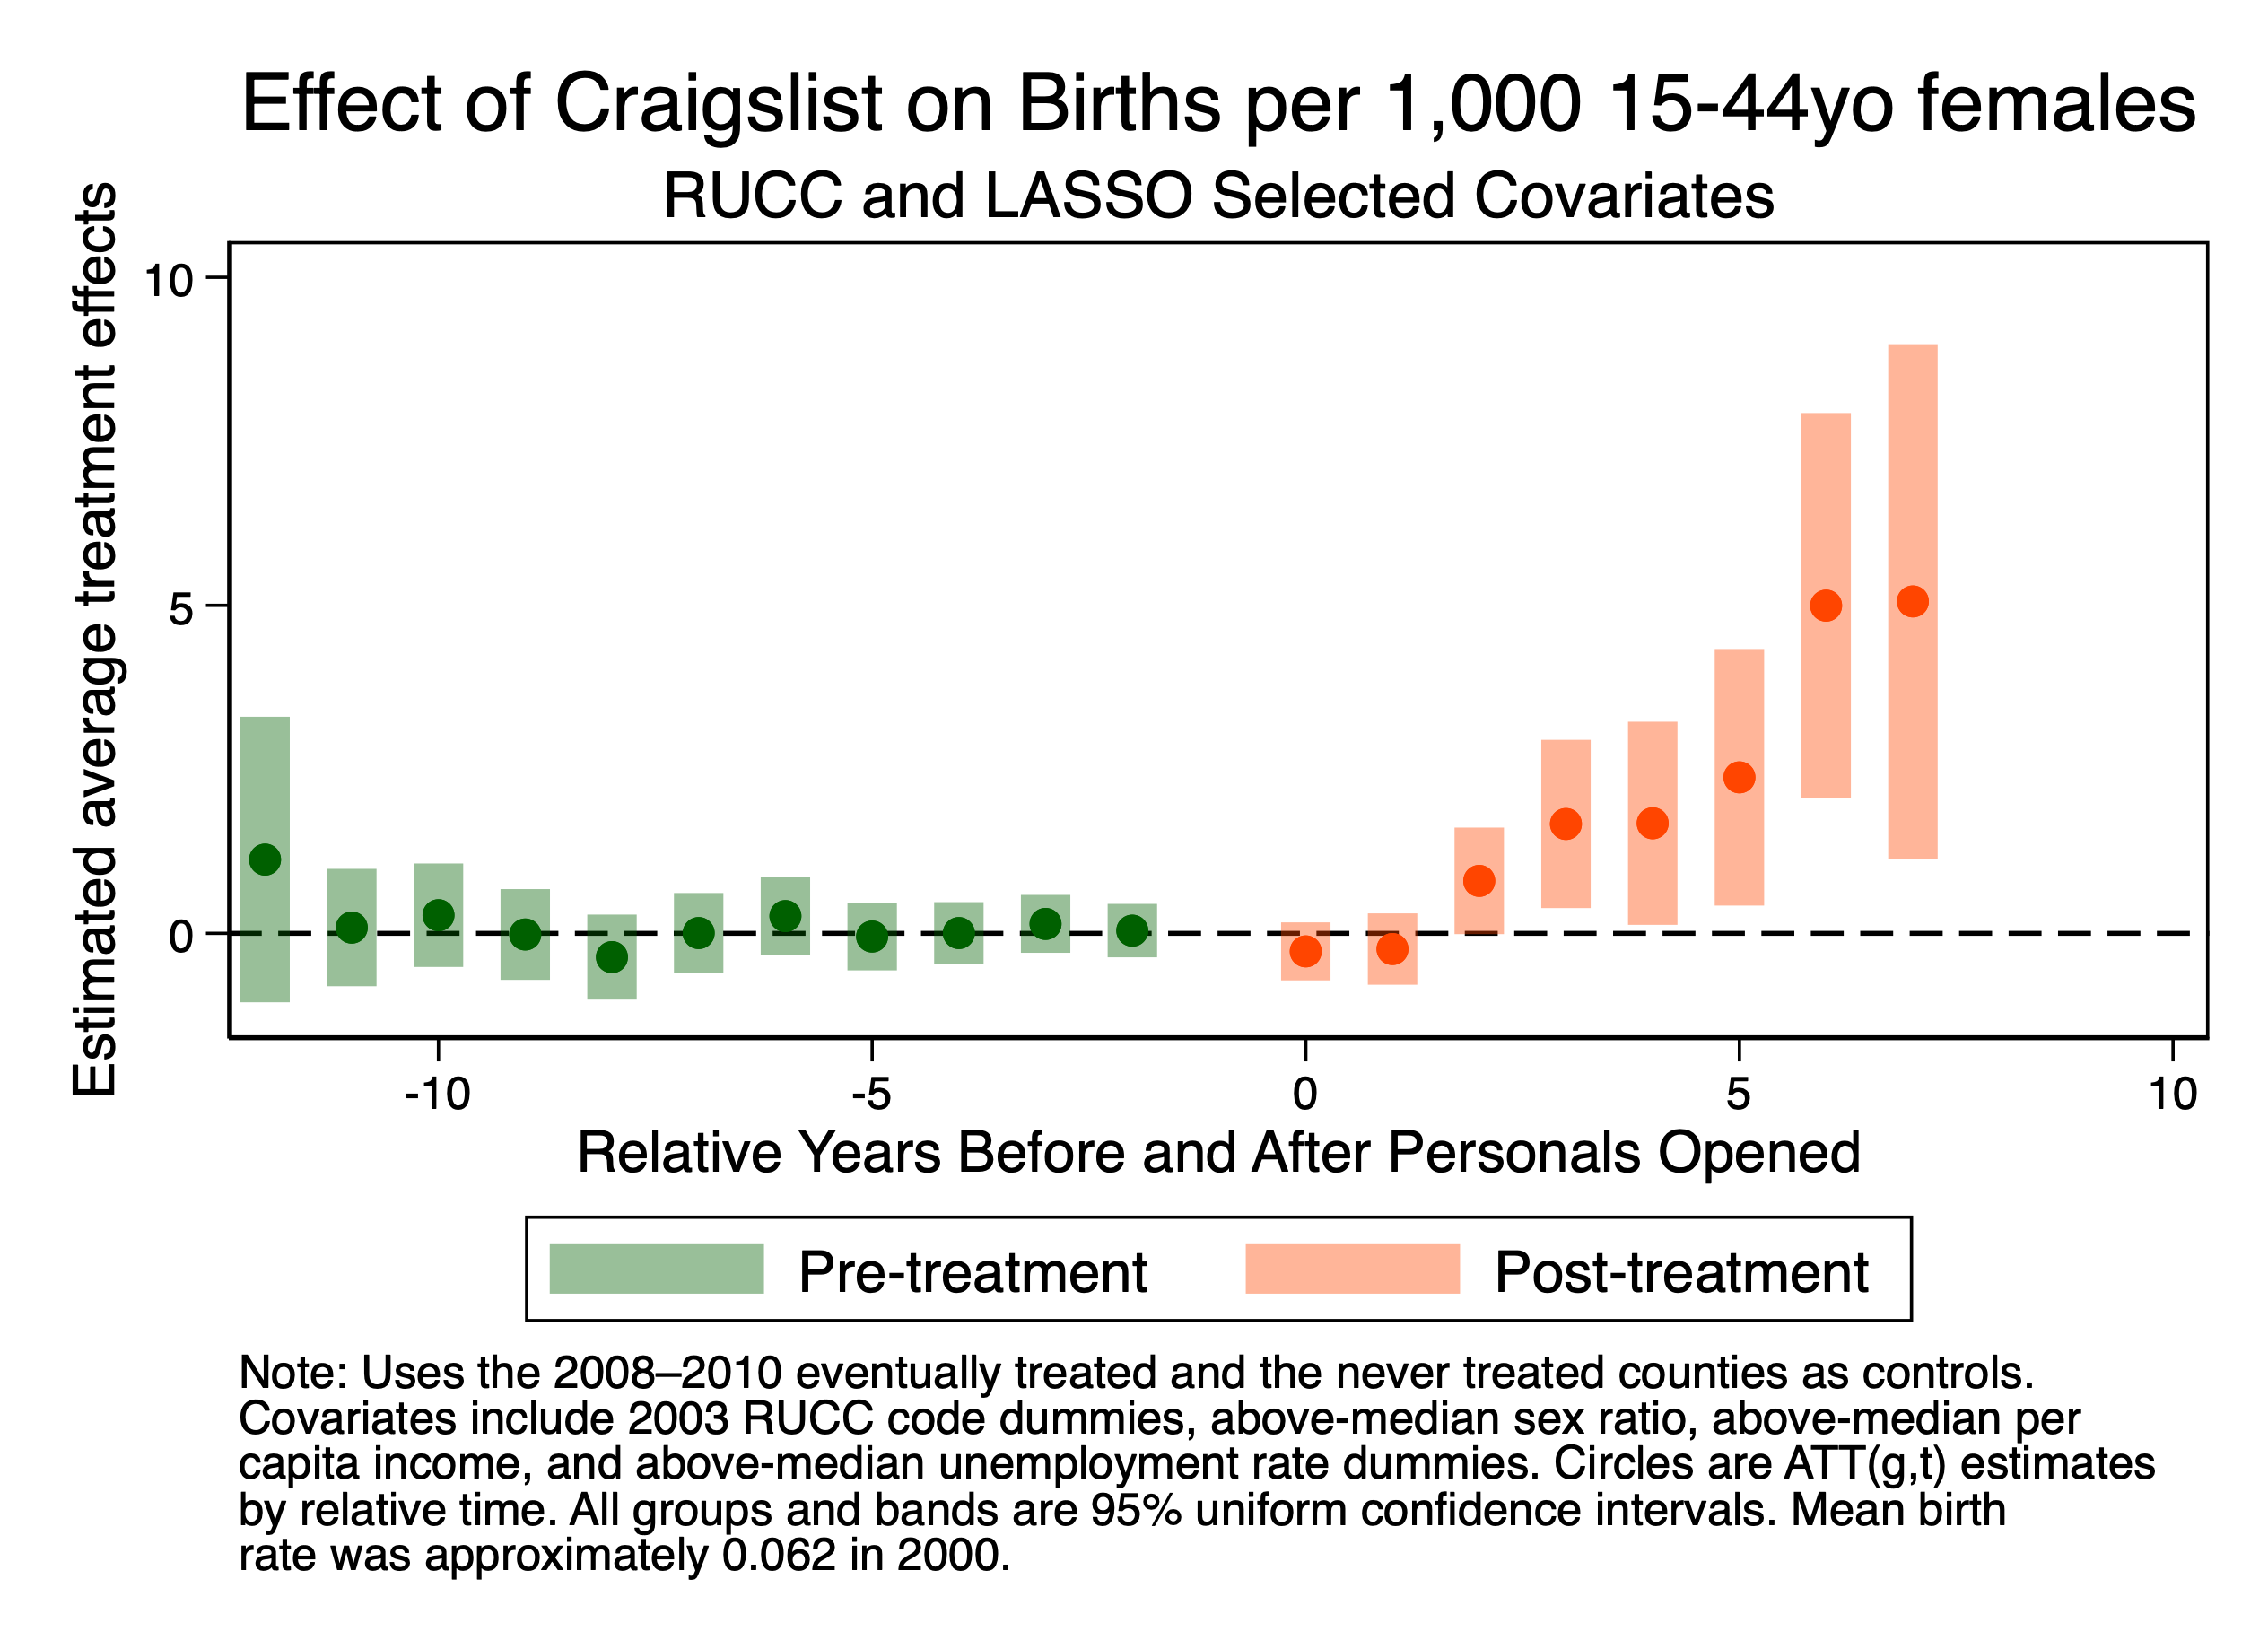
\includegraphics[height=0.85\textheight]{./lecture_includes/es_births_allX.png}
\end{figure}

\end{frame}

\begin{frame}{Interpreting those late lags}

\begin{itemize}
\item We have staggered rollout -- why does that matter?
\item All cohorts contribute $t=0$, but we lose one cohort at each lag
\item We don't find positive effects until 3rd lag and there's two things happening
	\begin{enumerate}
	\item On the one hand, it takes at least 9 months after meeting "the one" to have a child, so lags are reassuring
	\item On the other hand, CS is literally losing cohorts with each lag so mechanical sample selection
	\end{enumerate}

\end{itemize}

\end{frame}


\begin{frame}[shrink=20]{Number of counties by treatment cohorts}
\begin{table}[htbp]\centering
\caption{Number of counties by year Craigslist personals appeared}\label{tab:countybycohort}
\begin{tabular}{lc}
\toprule
\textbf{Treatment Cohort} & \textbf{Number of Counties Treated} \\
\midrule
Never treated&       1,779\\
2000 cohort &           9\\
2001 cohort &           5\\
2002 cohort &          12\\
2003 cohort &          36\\
2004 cohort &          58\\
2005 cohort &          69\\
2006 cohort &         341\\
2007 cohort &          65\\
2008 cohort &          66\\
2009 cohort &         215\\
2010 cohort &           1\\
\midrule
Total counties &     2,656 \\
\bottomrule
\end{tabular}
\end{table}
\end{frame}

\begin{frame}{Differentially sized cohorts}

\begin{itemize}
\item But there's more -- those "late adopters" are \emph{massive} which in CS is causing that alone them to shift the effects
\item Simple ATT is not significant with the 2006 cohort, but it is when it's gone
\item But it's just size -- those late adopters are \emph{rural}, they are \emph{much later}
\item Lots of different things about them and we are working on that now
\end{itemize}

\end{frame}


\begin{frame}{Writing this up will be horrible!}

\begin{itemize}

\item I don't mind showing you all this because it's a workshop about doing the work
\item Mark and Dan are going to talk about writing the papers!
\item But, we have \emph{no idea} how we are going to somehow collect all of this and make one coherent paper (we will be taking Mark and Dan's hidden curriculum workshop!)
\item Point is, though, that that's a different part of the process -- we want to understand \emph{mechanically} what CS is doing, \emph{numerically} the calculations (e.g., the weighting, the "dropping out cohorts")
\item We don't just want to jump to some gestation story in other words
\end{itemize}

\end{frame}



\begin{frame}{Be Curious, Not Judgment -- Ted Lasso}

\begin{itemize}

\item Do everything you can to figure out the treatment assignment mechanism 
\item Shoeleather dominates technical knowledge (Rubin 2008 "Design Trumps Analysis"; Freedman 1991)
\item Consider interviewing key people!  But don't ask them if they randomized -- they don't know what that word means
\item Ask them "hey, why did you do that thing you did?" or "hey, why did some people get put into your program but not others?"
\end{itemize}

\end{frame}

\begin{frame}[shrink=20]
    \centering
    \begin{center}
    \begin{figure}
        
\includegraphics[width=\textwidth]{./lecture_includes/craig_dm}
    \end{figure}
    \end{center}
    

    
\end{frame}




\section{Honest DiD}
'
\begin{frame}{Sensitivity Analysis}

\begin{itemize}
\item Assume the worst -- use the absolute worst gap in pre-trends and imagine PT broke by that much post-treatment
\item How bad does that have to get before your treatment effect coefficient covers zero?
\item Called \texttt{honestdid} by Rambachan and Roth (2023) 
\item Don't think of it as rejecting PT -- it's just saying how dependent on it you are
\end{itemize}

\end{frame}

\begin{frame}{Sensitivity Analysis}

	\begin{figure}
    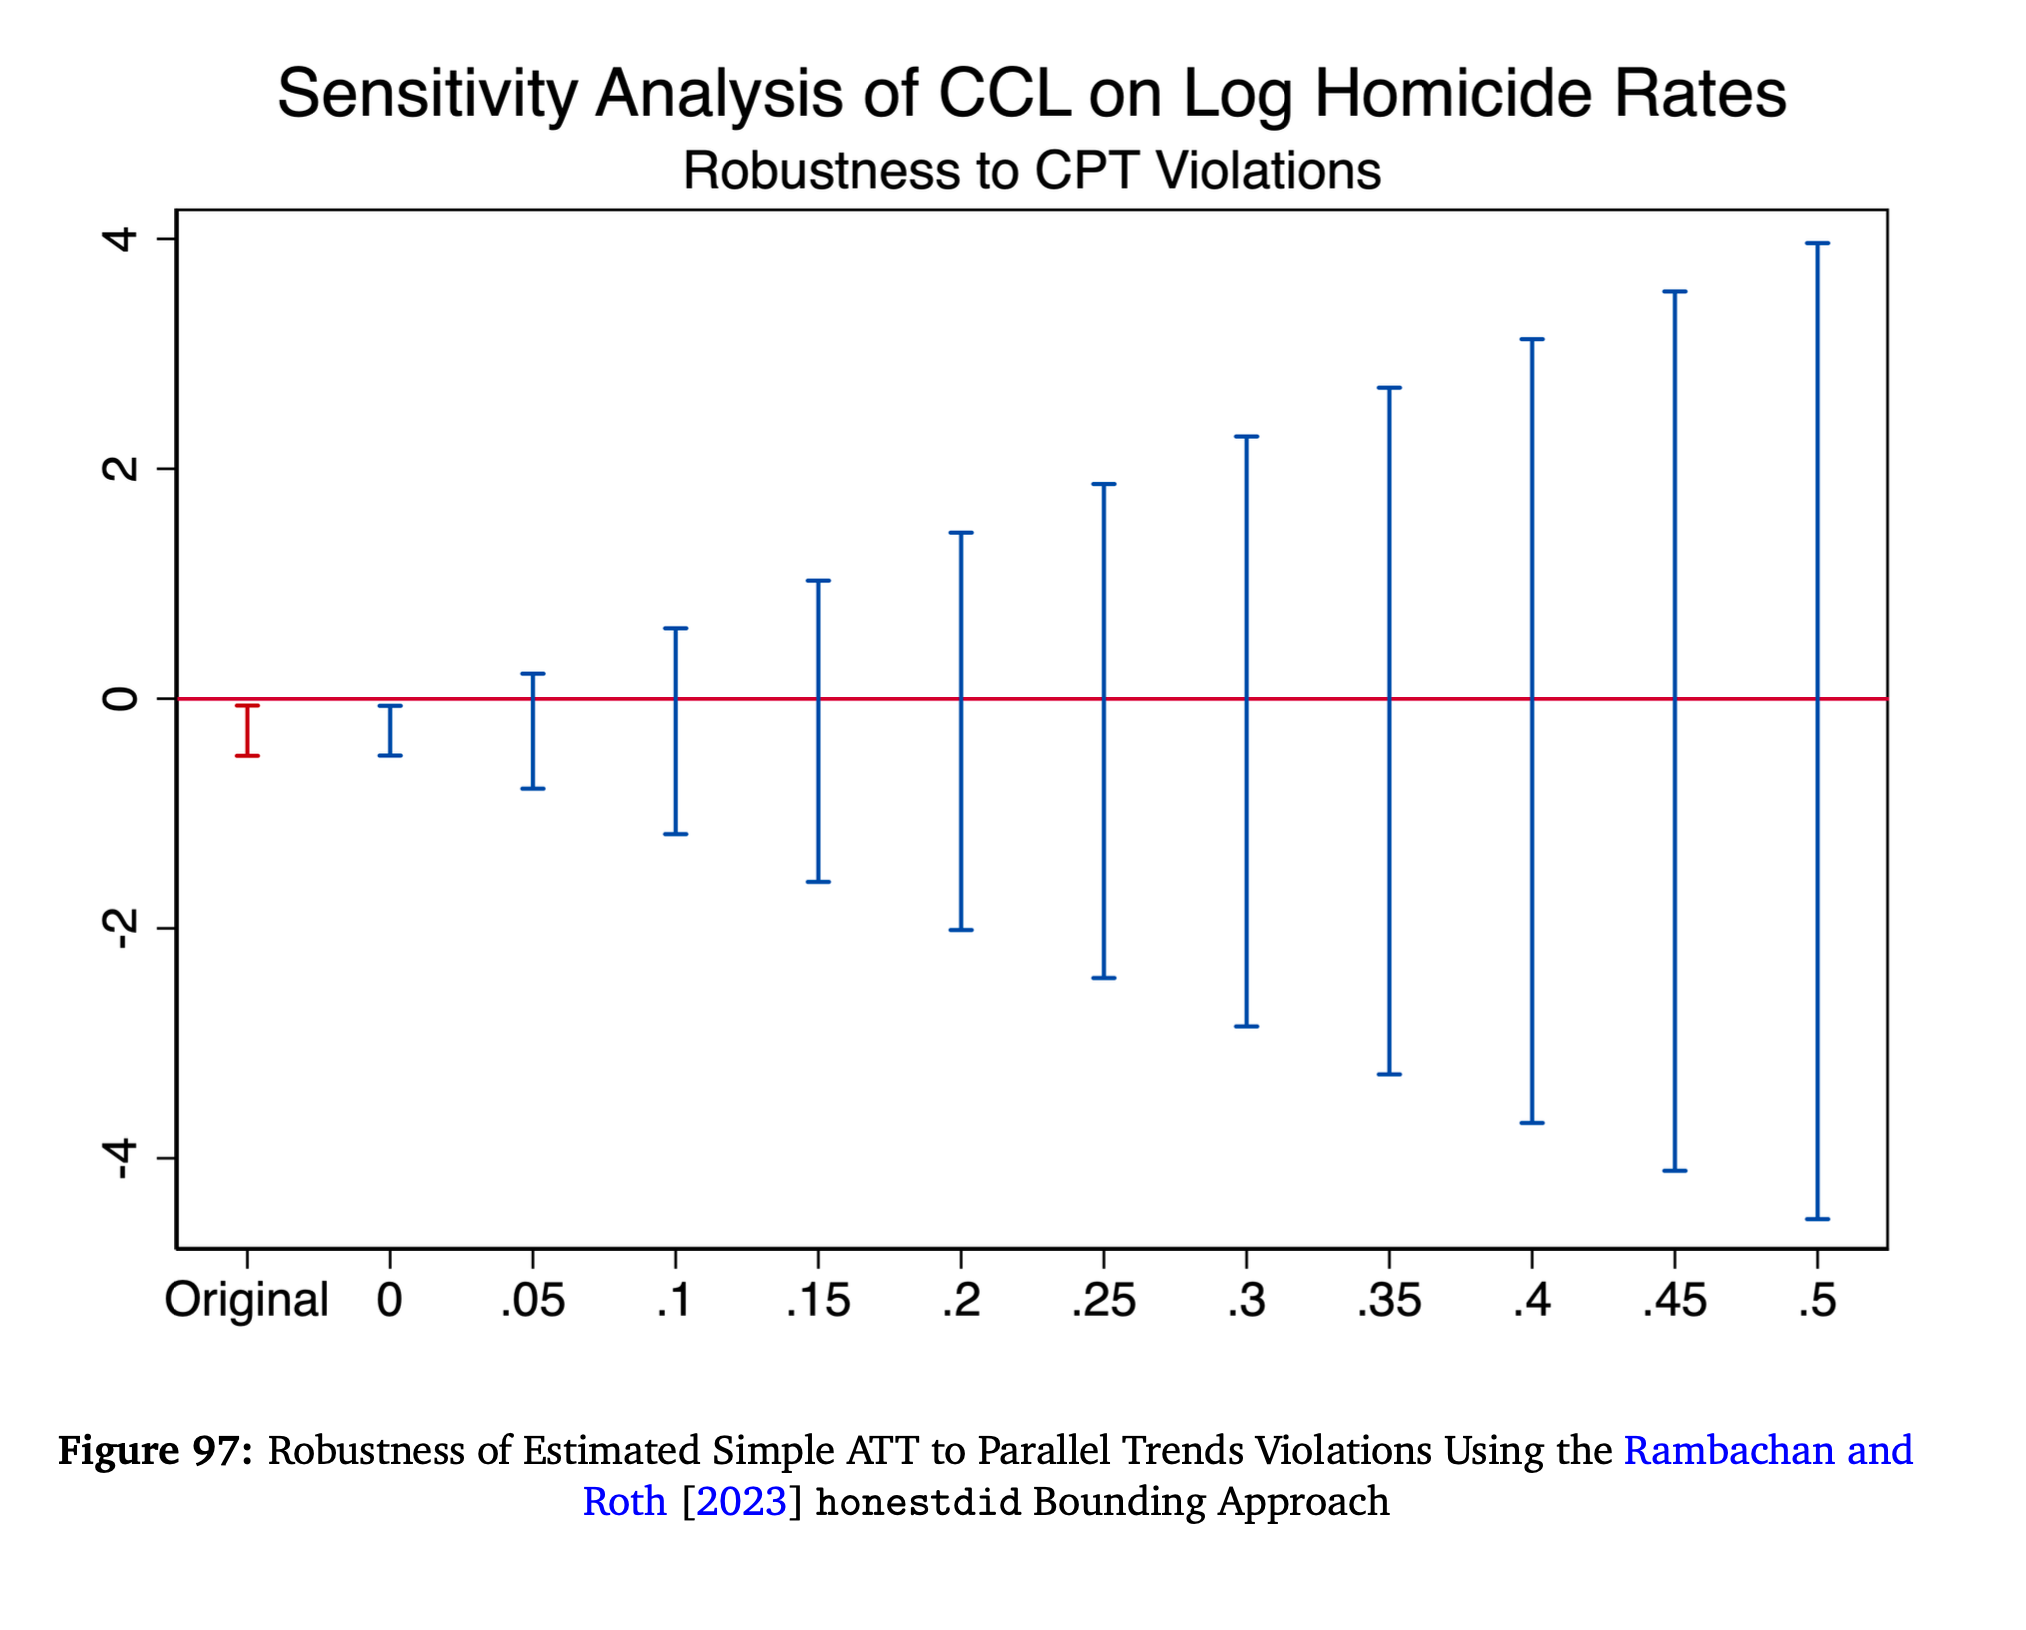
\includegraphics[height=0.85\textheight]{./lecture_includes/step9_roth}
	\end{figure}

\end{frame}






\section{DDDiD}





\begin{frame}{Final Step is to Do DDDiD}

\begin{itemize}
\item DDDiD is a powerful new estimator by Guido Imbens that you use when parallel trends doesn't hold
\pause
\item \textcolor{red}{"Don't Do Diff-in-Diff"}

\end{itemize}

\end{frame}

\begin{frame}{Goal was never to use diff-in-diff though}

\begin{itemize}
\item Chainsaws are amazing but that doesn't mean you should try to use them to sharpen pencils
\pause
\item If you simply do not believe parallel trends assumption holds in your data, for whatever reason, then diff-in-diff is the wrong estimator
\item Some things can be good for some stuff but not other things and that's okay
\item Besides --  our goal was never to use diff-in-diff 
\item Our goal was to get good, believable answers to good questions and then tell people about them in truthful, careful, non-confusing ways
\item Kyle is going to talk about imputation estimators as alternatives to diff-in-diff!

\end{itemize}

\end{frame}





\end{document}

\subsection{Example from AER 2022: Mental Health and Social Media}

\begin{frame}
\begin{center}
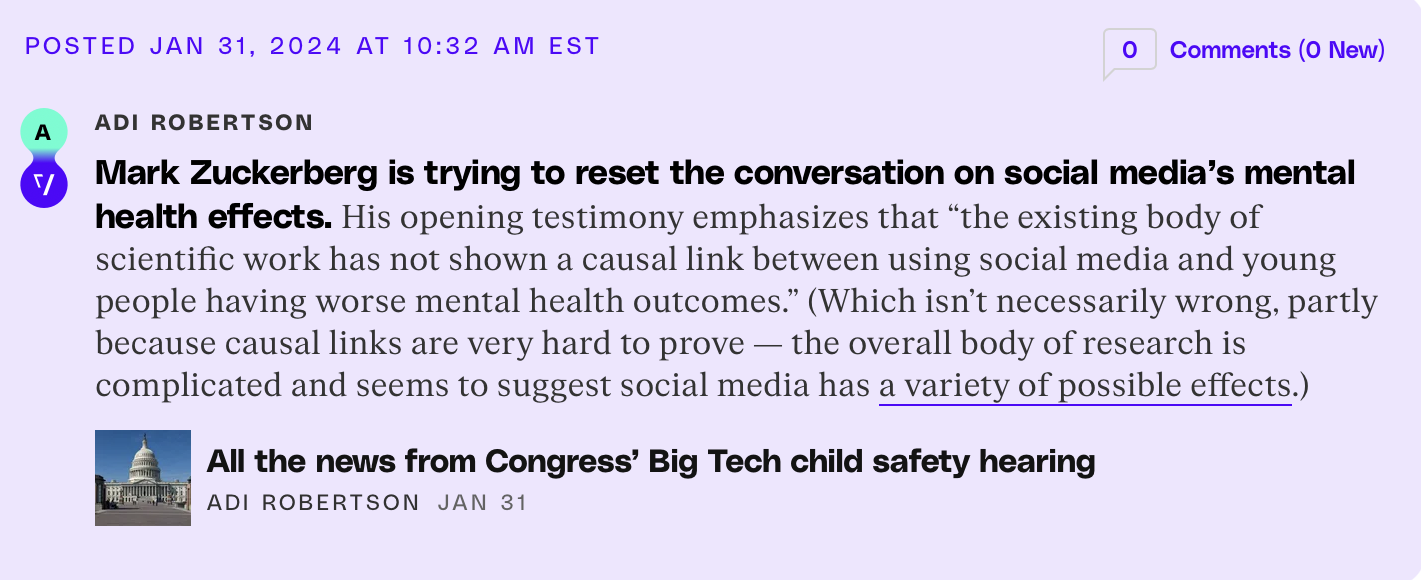
\includegraphics[scale=0.35]{./lecture_includes/facebook_quote}
\end{center}
\end{frame}



\begin{frame}{Mental health and Social Media}

\begin{itemize}
\item Unclear what he means; he may mean there is no experimental evidence
\item Very difficult to imagine a randomized experiment -- especially once the claim out there is that it is harmful, Institutional Review Boards likely wouldn't approve it
\item Quasi-experimental evidence can step in to answer important questions like this
\item Braghieri, Levy and Makarin (2022), ``Social Media and Mental Health'', \emph{American Economic Review}, 112(11): 3660-3693


\end{itemize}

\end{frame}

\begin{frame}{Overview of design and data}

\begin{itemize}
\item Authors take advantage of a clever quirk in Facebook (then ``theFacebook'') targeted different universities from 2004 to 2006
\item They found an online data source that allowed them to pin point precisely when a university was ``treated'' with theFacebook
\item They then linked that data with a longrunning health survey of college students (both before and after) in a very clever way
\item Estimated the effect of a new social media platform's presence at a university on student revealed mental health problems

\end{itemize}

\end{frame}


\begin{frame}{DID in Court}

Five elements of a strong DiD
\begin{enumerate}

\item \textbf{Bite}: \textcolor{red}{Nothing}. They cannot really show much here.  No data on Facebook usage.  They had to rely on anecdote and Facebook as a ``first mover'', but there had been Friendster and MySpace so this does weaken the paper maybe
\item \textbf{Main Results}: Very strong evidence, mostly expressed using rich survey data and questions transformed into z-scores (standard deviations)
\item \textbf{Falsifications}: \textcolor{red}{None}. Authors do not perform falsifications. Remember Miller, Johnson and Wherry looking at Medicaid's effect on Medicare eligible population?  There isn't anything like that here.
\item \textbf{Event studies}: Extremely compelling evidence and robustness across a half dozen different models
\item \textbf{Mechanism}: \textcolor{red}{Very weak in my opinion}

\end{enumerate}

\end{frame}

\begin{frame}{DiD in Court}

\begin{itemize}

\item So in many ways the strength of the project lies in a few areas:
	\begin{enumerate}
	\item Important question -- social media and youth mental health problems is a major policy question (see Zuckerberg testifying before Congress about it)
	\item Excellent research design -- difference-in-differences
	\item Meticulous data collection
	\item Data visualization is compelling
	\end{enumerate}
\item And it publishes in the premiere journal in economics, which I think shows that the research question and high quality data combined with research design can lift a paper

\end{itemize}

\end{frame}







\begin{frame}{TWFE}

\begin{equation}
Y_{icgt} = \alpha_g + \delta_t + \beta \times Facebook_{gt} + X_i \times \gamma + X_c \times \psi + \varepsilon_{icgt}
\end{equation}

\bigskip

This is a version of the regression model we looked at called "twoway fixed effects".  Somewhat complicated to dig into, so I will just say that they use it plus some other methods that are appropriate when you have several difference-in-differences events.  But the focus is on $\beta$

\end{frame}


\begin{frame}{Data on Facebook}

\begin{itemize}

\item When does Facebook appear at a school?  
	\begin{itemize}
	\item Facebook only publishes a fraction of that information
	\item They came up with a workaround
	\end{itemize}
\item The Wayback Machine has been taking almost daily photographs of every website since the Internet's beginning -- including the frontpage of ``TheFacebook''
\item Guess what was on the front page of TheFacebook \dots

\end{itemize}

\end{frame}

\begin{frame}
\begin{center}
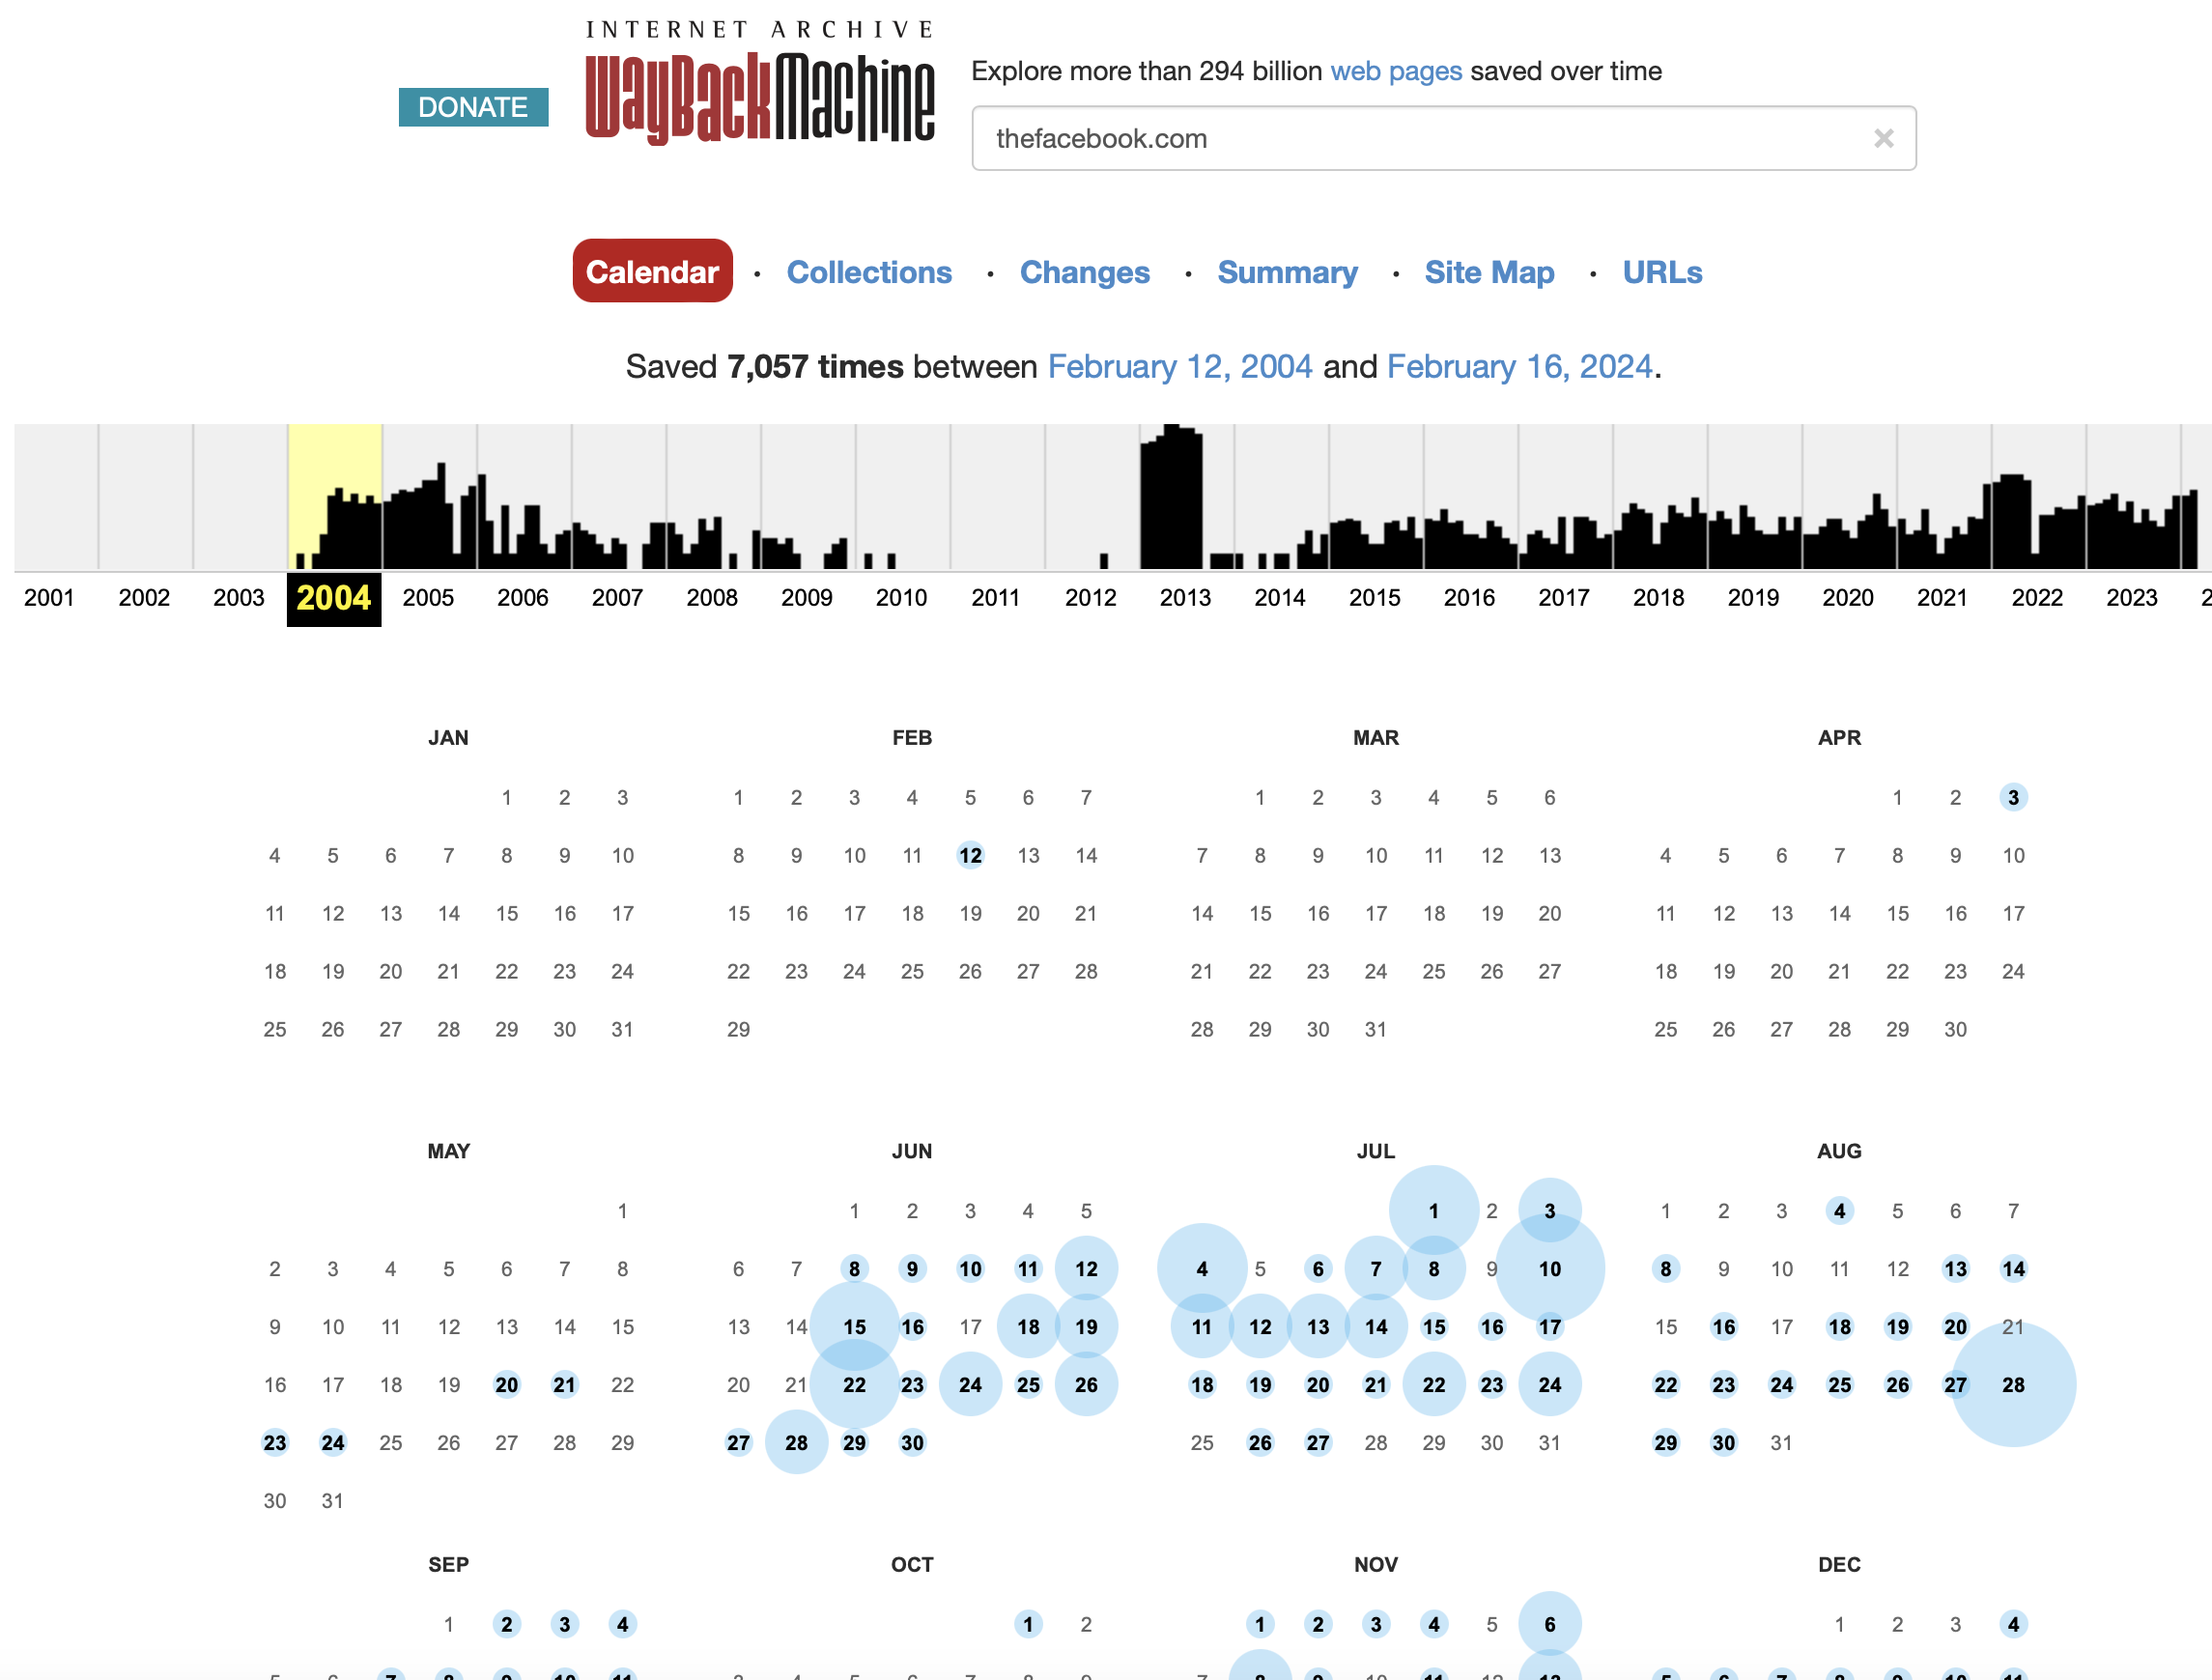
\includegraphics[scale=0.25]{./lecture_includes/wayback1}
\end{center}
\end{frame}

\begin{frame}
\begin{center}
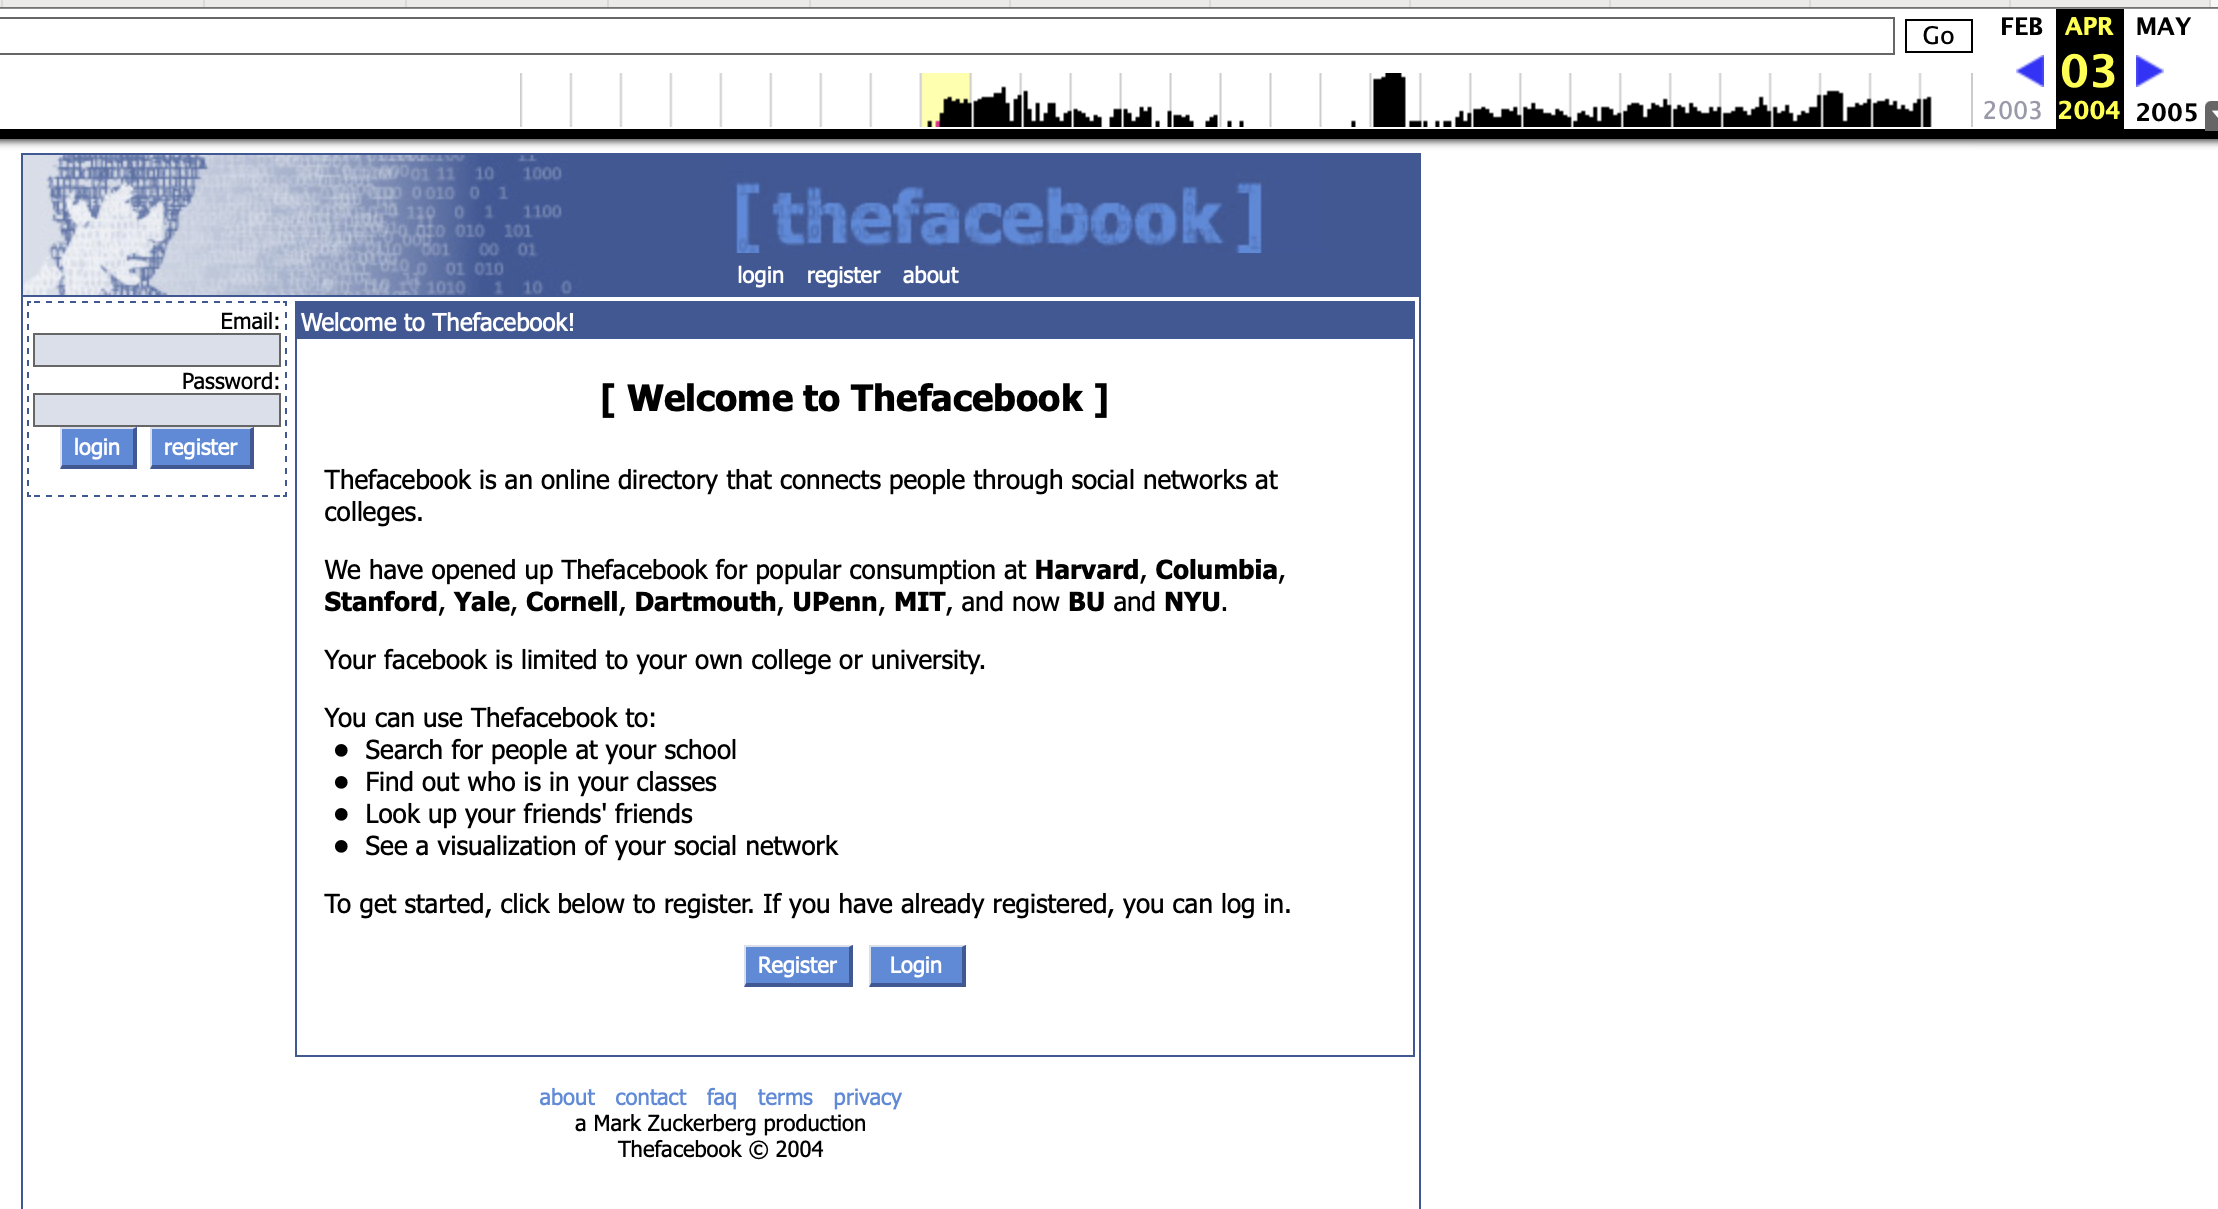
\includegraphics[scale=0.35]{./lecture_includes/wayback2}
\end{center}
\end{frame}

\begin{frame}
\begin{center}
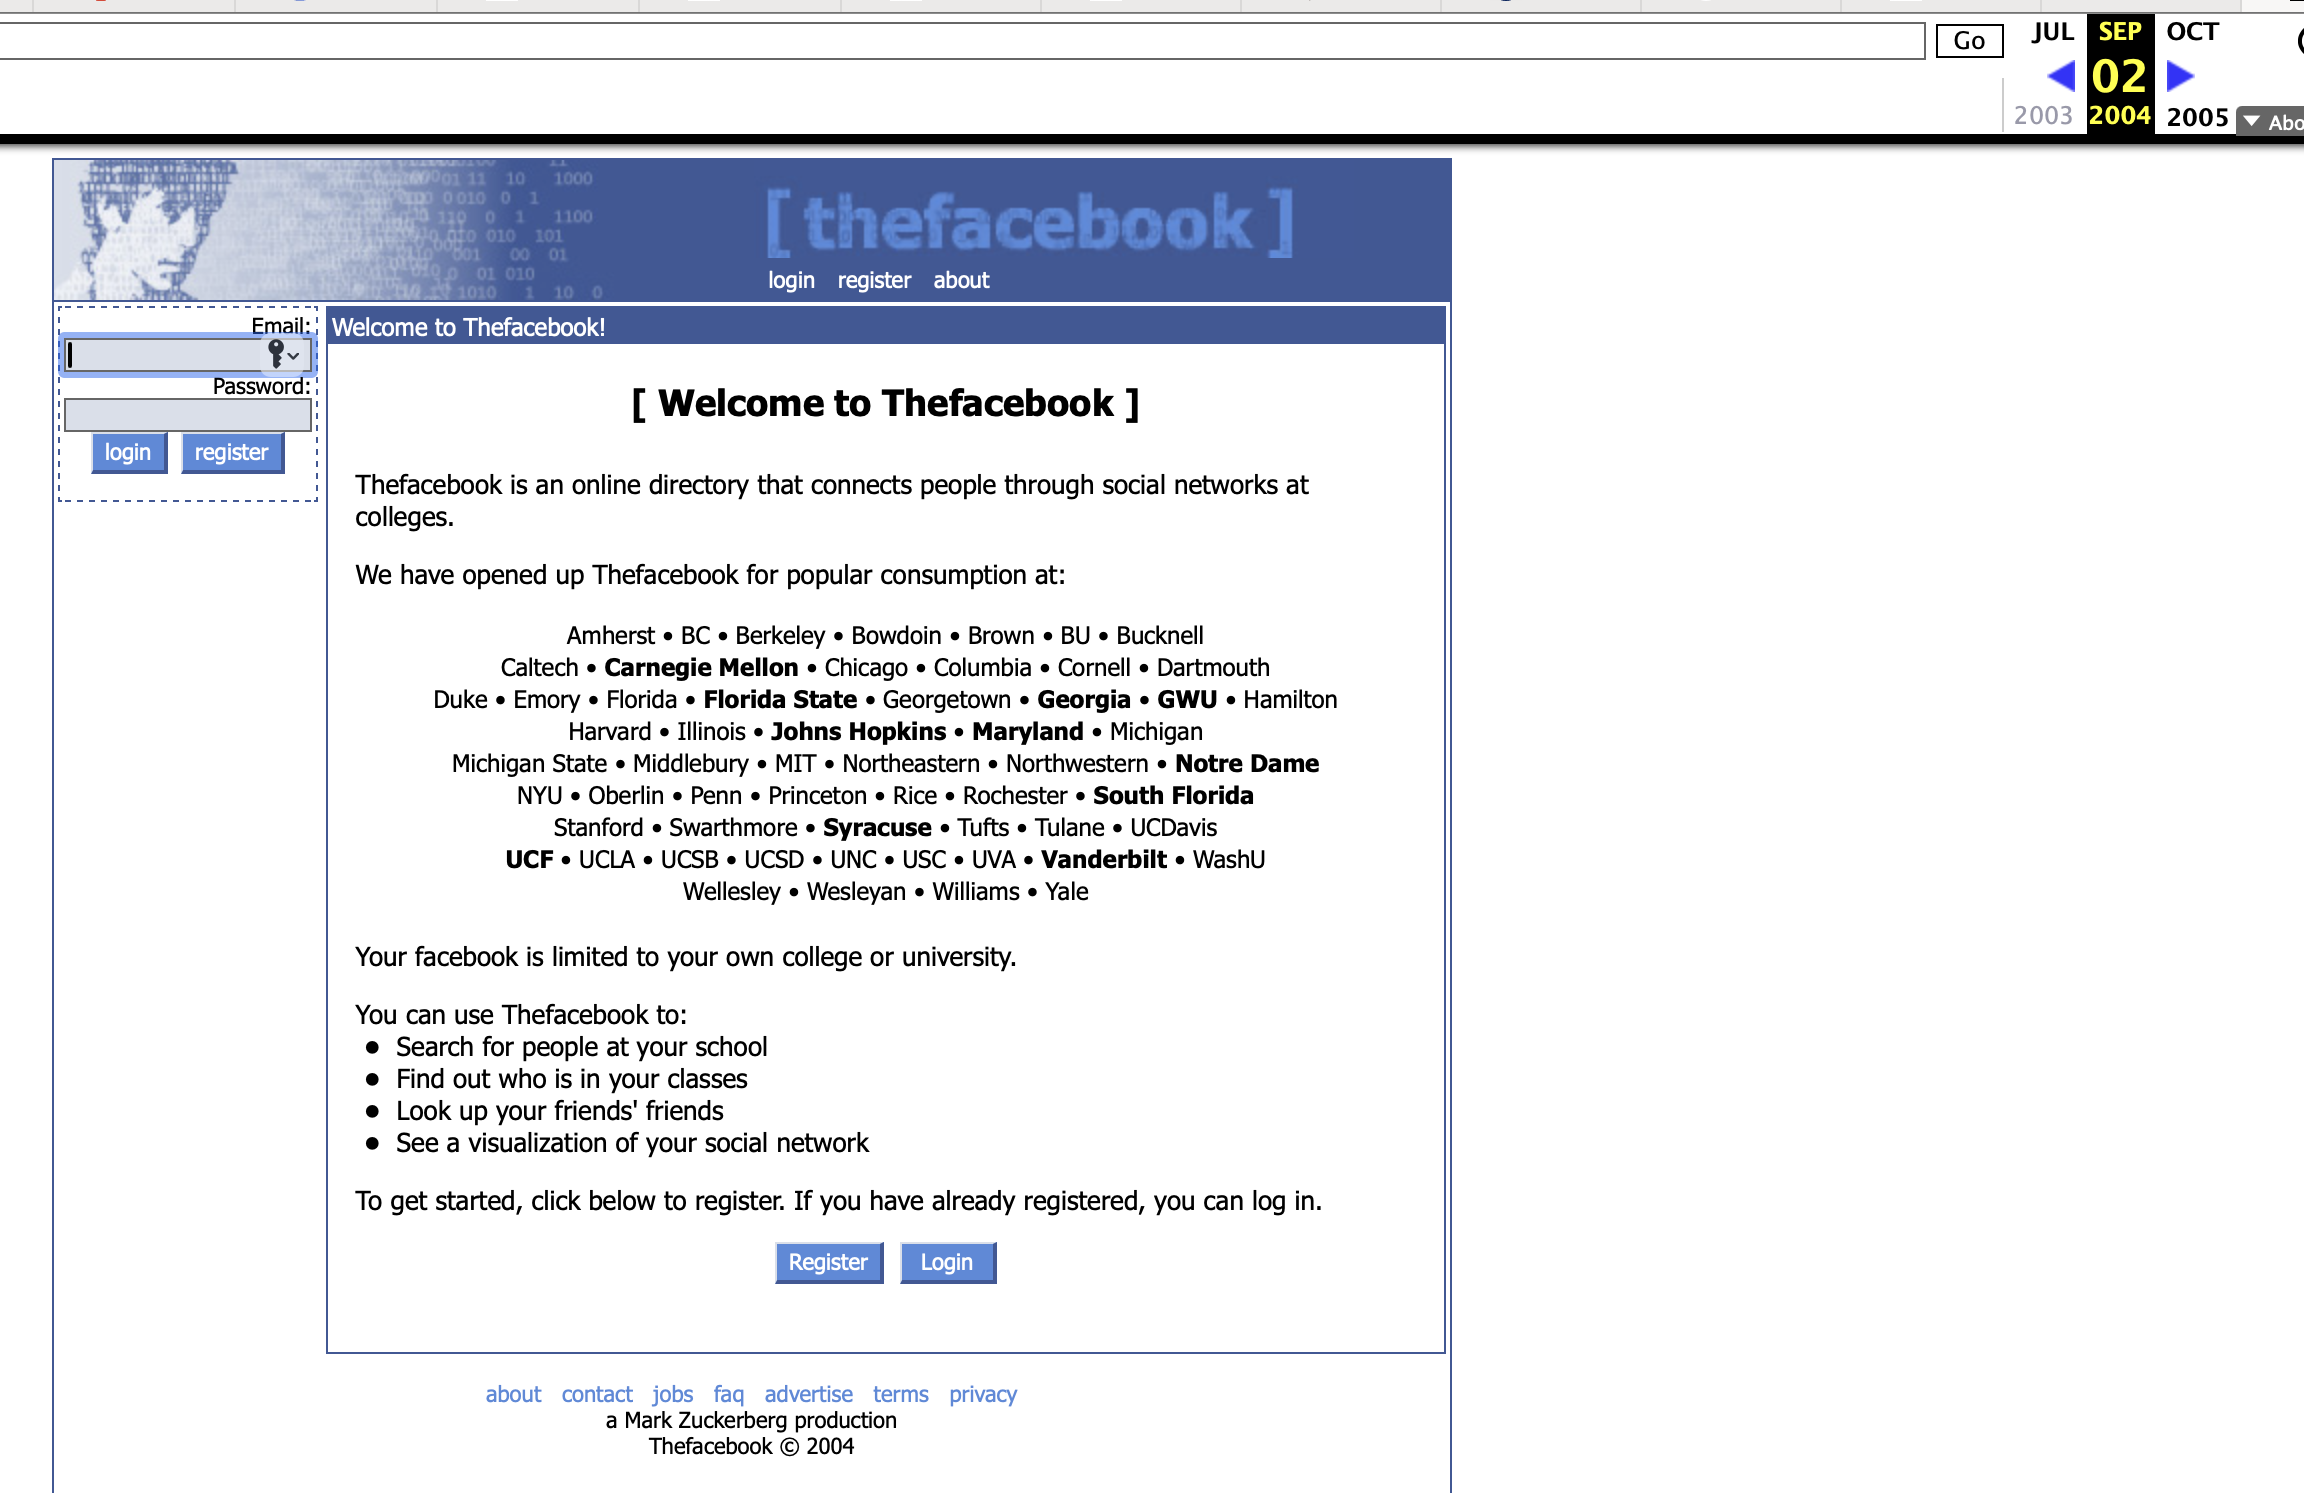
\includegraphics[scale=0.25]{./lecture_includes/wayback3}
\end{center}
\end{frame}

\begin{frame}
\begin{center}
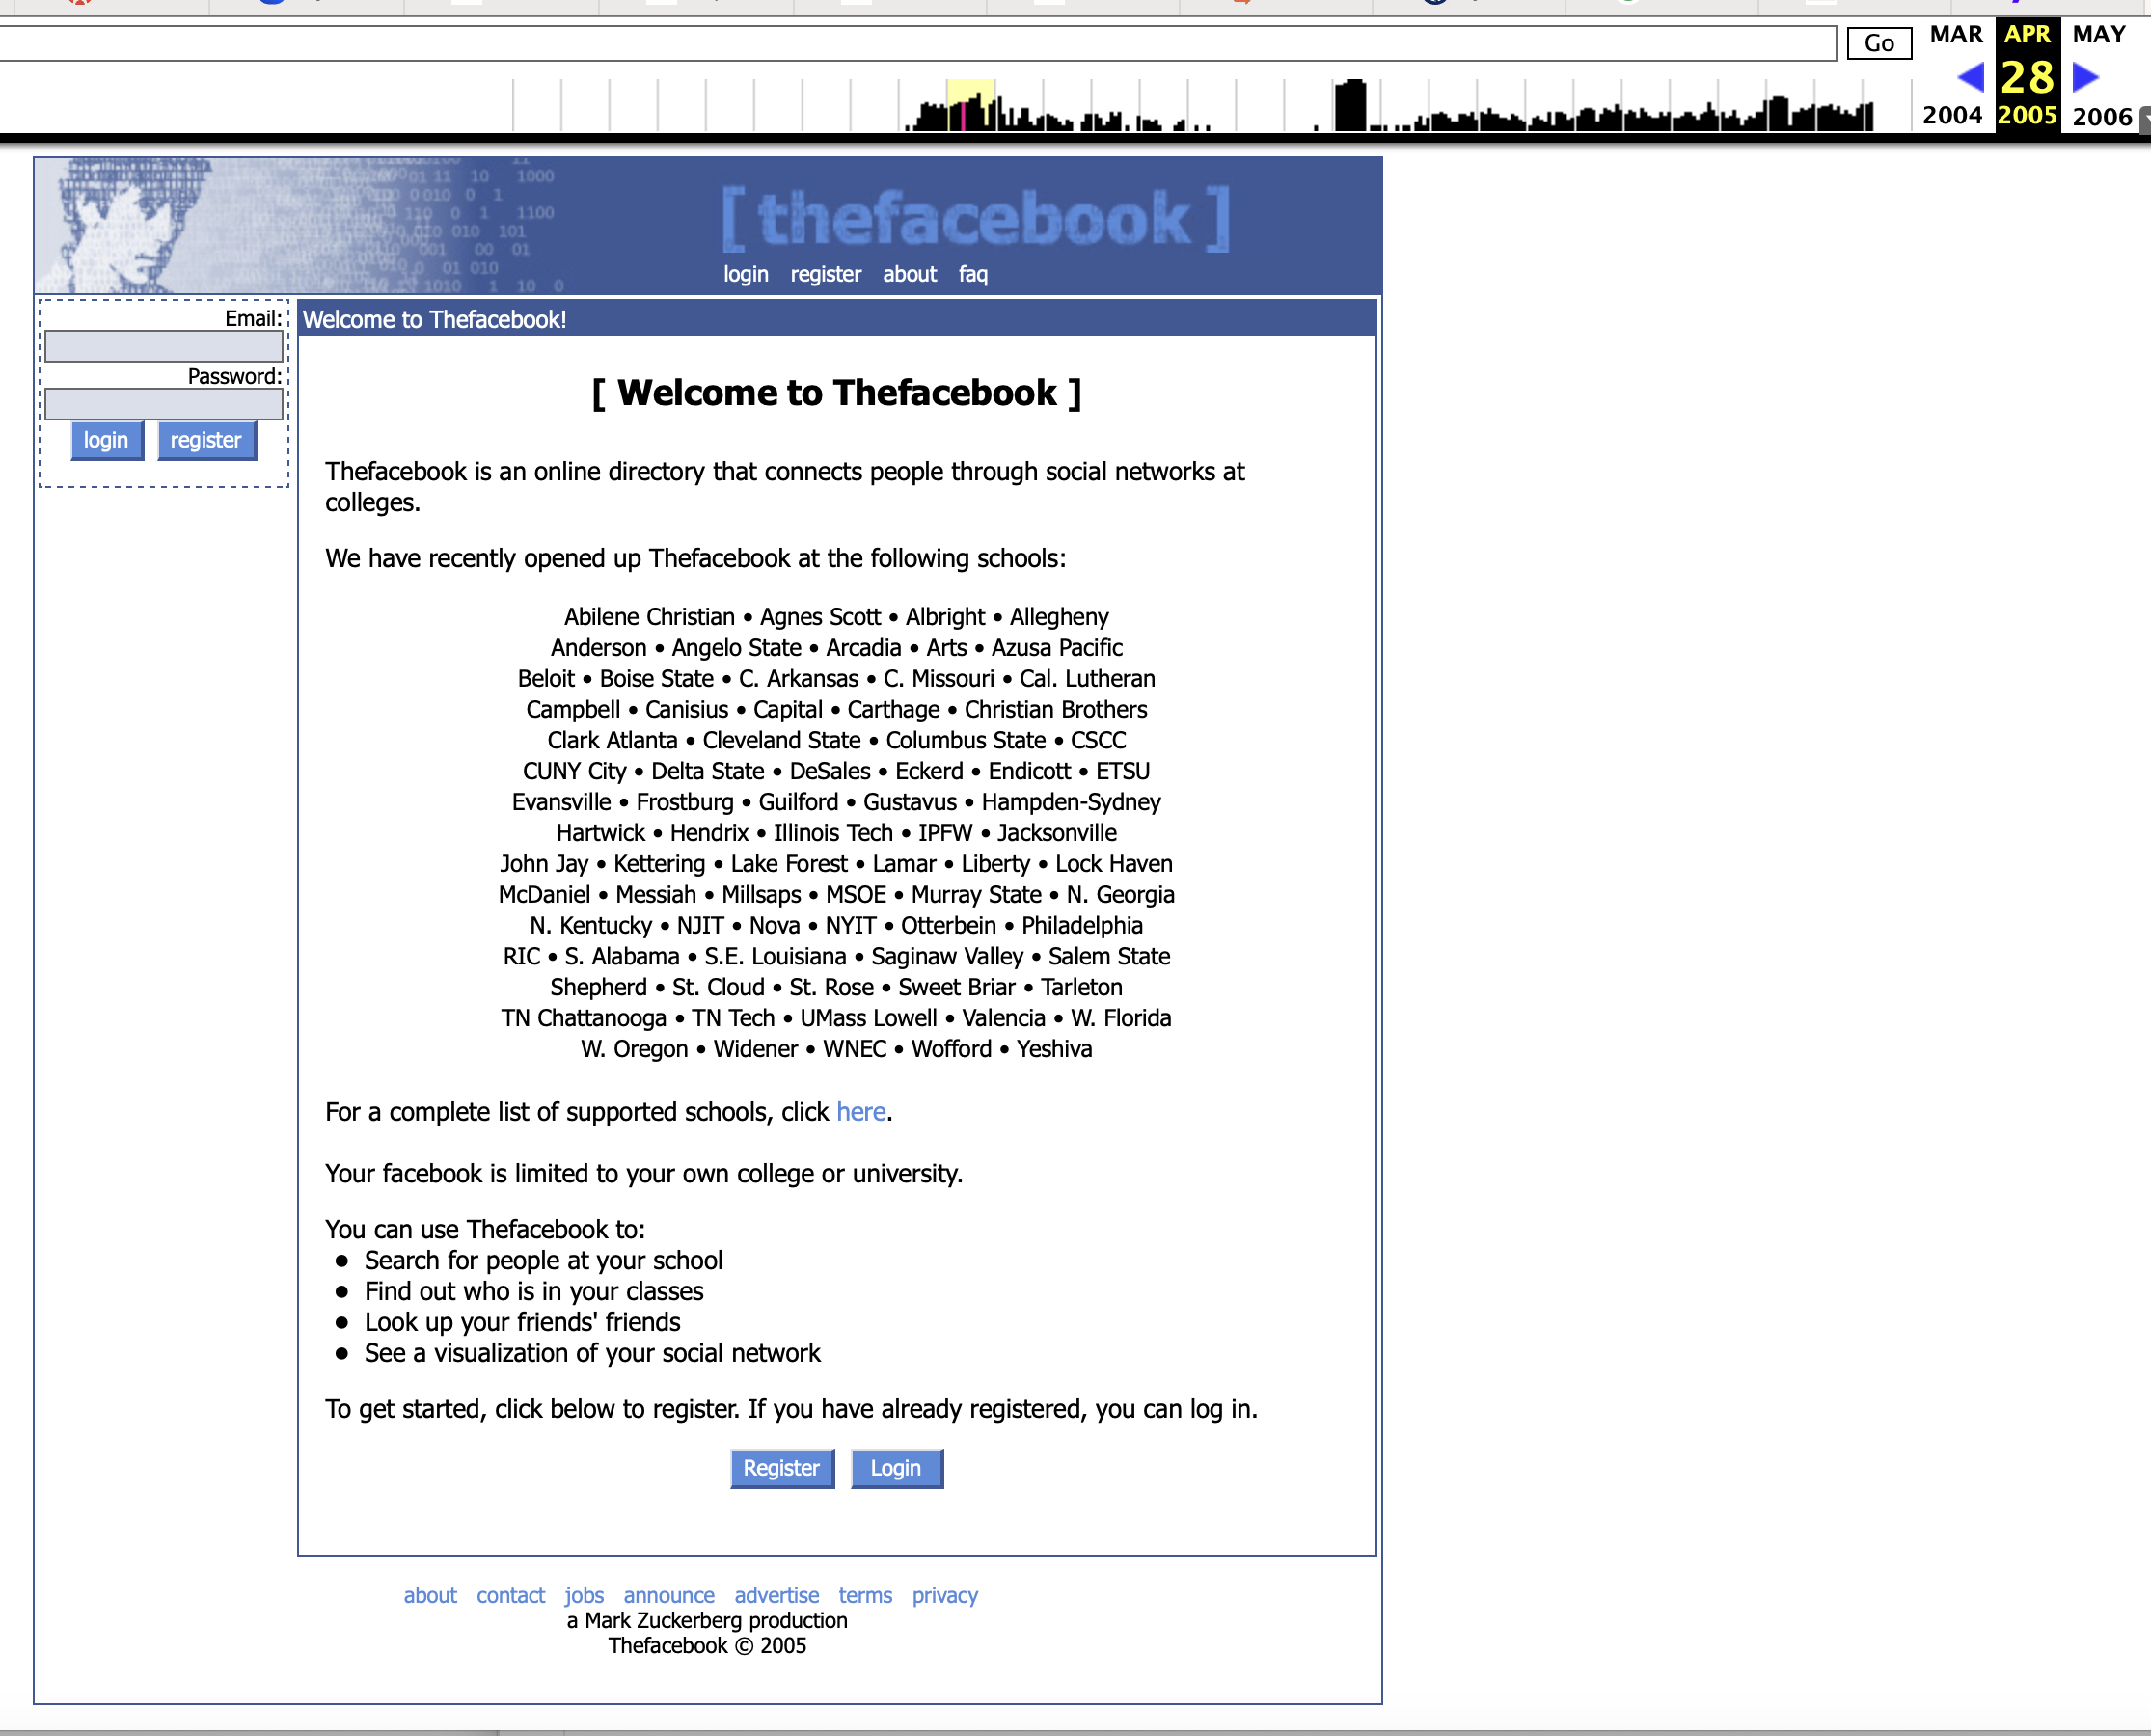
\includegraphics[scale=0.25]{./lecture_includes/wayback4}
\end{center}
\end{frame}

\begin{frame}{Timing Dates}

\begin{itemize}
\item They went through three years of daily screenshots on Wayback machine to find when a school appeared on the front page
\item The first time Agnes Scott, or Covenant, appears on the front page, the authors mark that as the date when the school got Facebook
\item But now they need information on mental health outcomes
\item They find it with an old long running repeated cross section survey of college students
\end{itemize}

\end{frame}

\begin{frame}{NCHA survey by ACHA}

\begin{quote}
Our second main data source consists of more than 430,000 responses to the NCHA survey, a survey administered to college students on a semi-annual basis by the American College Health Association (ACHA). The NCHA survey was developed in 1998 by a team of college health professionals with the purpose of obtaining information from college students about their mental and physical health. Specifically, the NCHA survey inquires about demographics, physical health, \textbf{mental health}, alcohol and drug use, sexual behaviors, and perceptions of these behaviors among one’s peers.
\end{quote}

\end{frame}

\begin{frame}{No evidence of bite}

\begin{quote}
The NCHA survey does not include any questions on social media use; therefore, it is not possible for us to determine whether a particular survey respondent had a Facebook account.
\end{quote}

\bigskip

This is probably the problem in any study in which your treatment is more or less the first of its kind -- most likely the standard surveys have not yet incorporated the questions into their surveys

\end{frame}

\begin{frame}{Linking Facebook data with NCHA data}

\begin{quote}
In order to protect the privacy of the institutions that participate in the NCHA survey while still allowing us to carry out the analysis, the ACHA kindly agreed to provide us with a customized dataset that includes a variable indicating the semester in which Facebook was rolled out at each college. Specifically, the ACHA adopted the following procedure: (i) merge our dataset containing the Facebook introduction dates to the NCHA dataset; (ii) add a variable listing the semester in which Facebook was rolled out at each college;15 (iii) strip away any information that could allow us to identify colleges (including the specific date in which Facebook was introduced at each college).
\end{quote}

\end{frame}

\begin{frame}{Basic facts about early and late adopters}

\begin{itemize}
\item Colleges in earlier Facebook expansion groups are more selective in terms of test scores, larger, more likely to be on the East Coast, and have more residential undergraduate programs than colleges in later Facebook expansion groups. 

\item Colleges in earlier Facebook expansion groups enroll students from relatively more advantaged economic backgrounds. 

\item Students in colleges that received Facebook relatively earlier have worse baseline mental health outcomes than students attending colleges in later Facebook expansion groups. 

%The baseline differences across Facebook expansion groups may lead one to wonder about the plausibility of the parallel trends assumption in this setting; we address concerns related to parallel trends in Section III.

\end{itemize}

\end{frame}

\begin{frame}{Measurement}

\begin{itemize}
\item The survey data is very rich with a lot of questions about mental health with different scales
\item They create their own combinations of these questions into aggregate indices -- ``index of poor mental health'' where higher numbers mean worse mental health
\item Each outcome survey question is normalized into what is called a ``z-score'' which is interpreted as a fraction of a standard deviation
\item Estimates are ATT parameters -- average effect of Facebook on students at schools that got Facebook
\end{itemize}

\end{frame}


\begin{frame}
\begin{center}
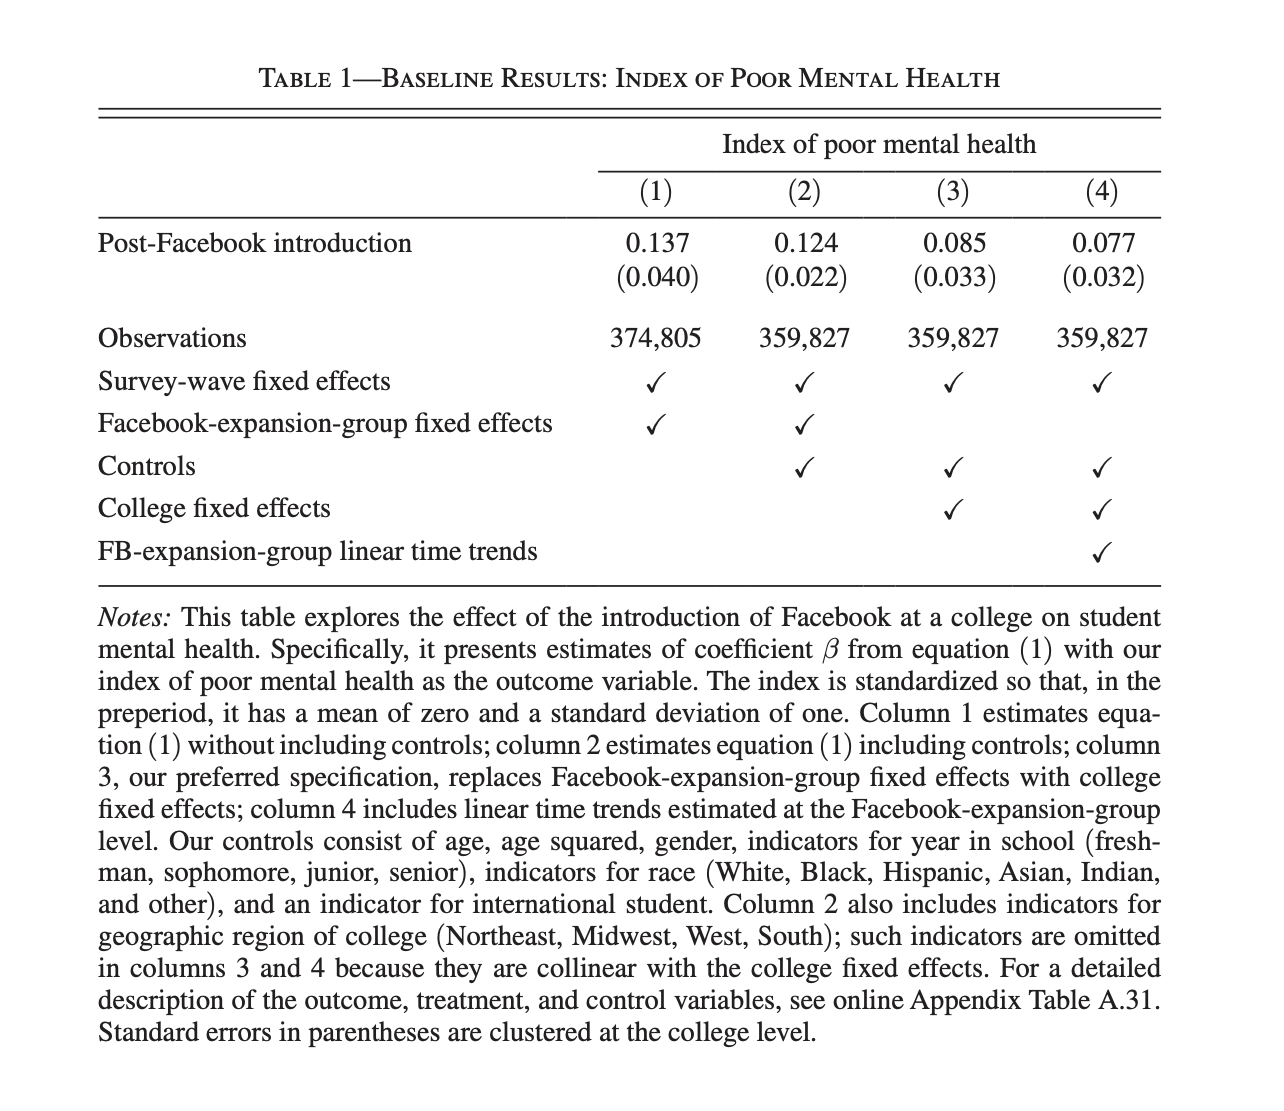
\includegraphics[scale=0.35]{./lecture_includes/facebook_1}
\end{center}
\end{frame}

\begin{frame}
\begin{center}
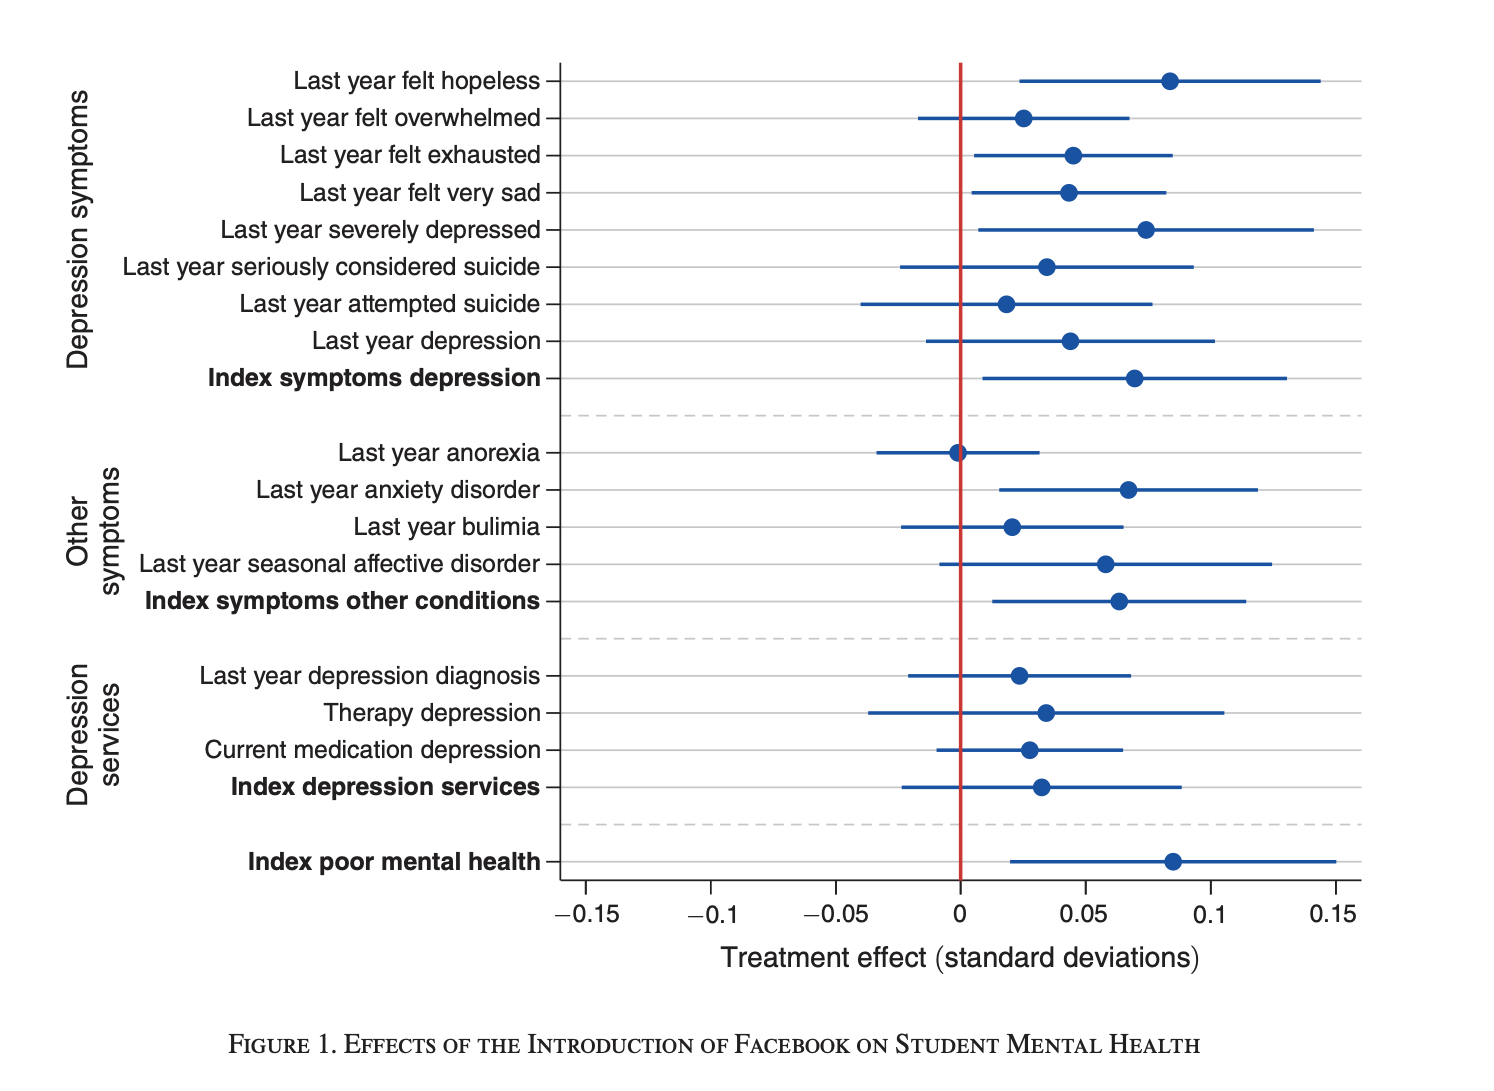
\includegraphics[scale=0.35]{./lecture_includes/facebook_2}
\end{center}
\end{frame}

\begin{frame}
\begin{center}
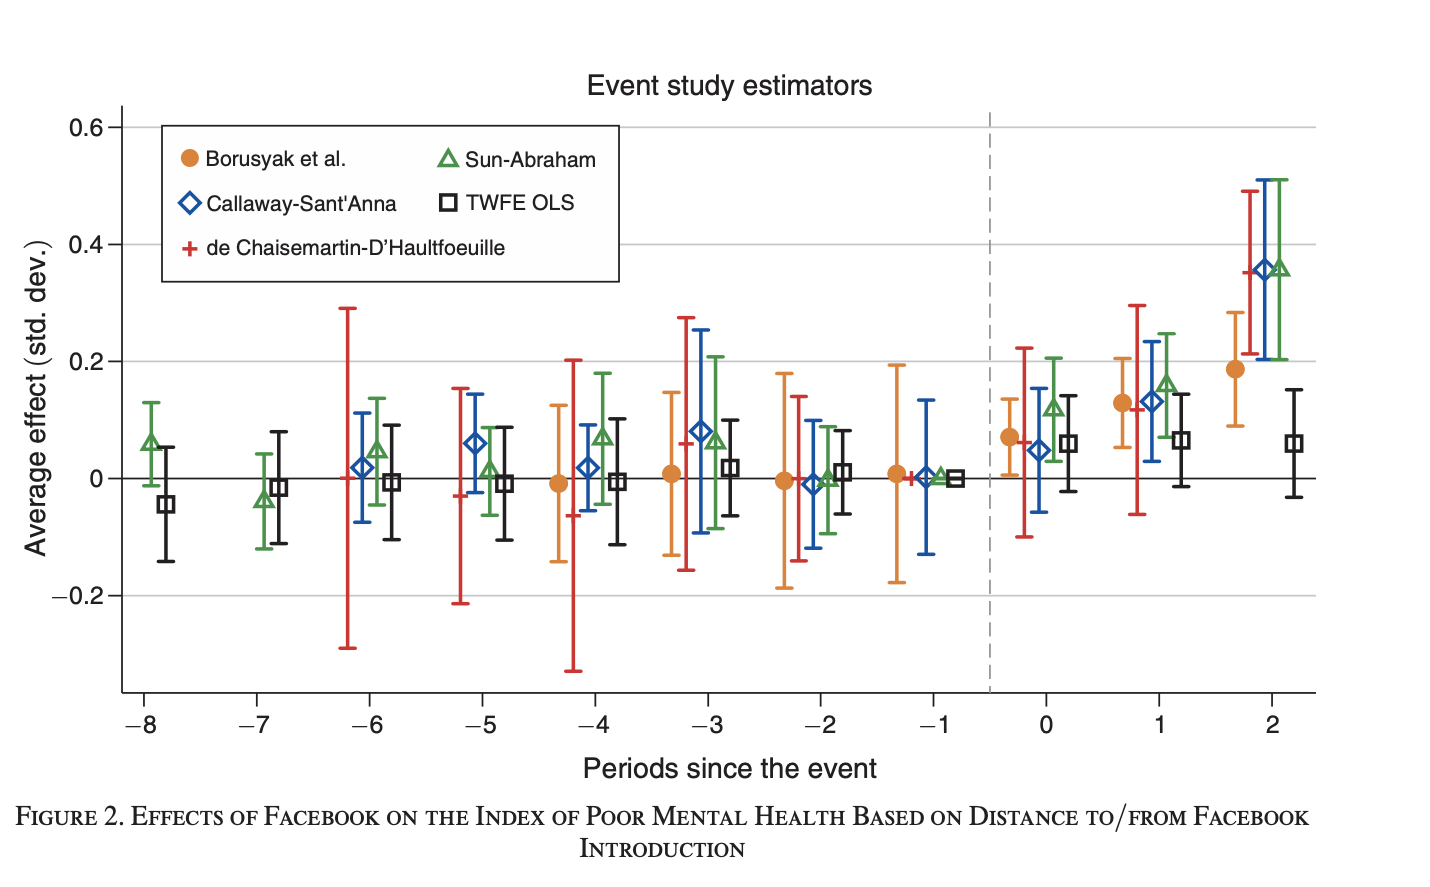
\includegraphics[scale=0.35]{./lecture_includes/facebook_3}
\end{center}
\end{frame}

\begin{frame}
\begin{center}
\includegraphics[scale=0.35]{./lecture_includes/facebook_4}
\end{center}
\end{frame}

\begin{frame}
\begin{center}
\includegraphics[scale=0.35]{./lecture_includes/facebook_5}
\end{center}
\end{frame}

\begin{frame}
\begin{center}
\includegraphics[scale=0.35]{./lecture_includes/facebook_6}
\end{center}
\end{frame}

\begin{frame}
\begin{center}
\includegraphics[scale=0.35]{./lecture_includes/facebook_7}
\end{center}
\end{frame}




\begin{frame}{Comparing them}

\begin{itemize}
\item Aggregating group-time ATT(g,t)
	\begin{itemize}
	\item CS and SA have the most flexible parallel trends assumption
	\item CS imposes no homogeneity restrictions with respect to covariates
	\item CS estimates a propensity score or nonparametric outcome regression to handle covariates so if you have poor overlap, it'll be biased even with conditional PT
	\end{itemize}
\item Imputation
	\begin{itemize}
	\item BJS is efficient with spherical errors (fat chance)
	\item BJS and Wooldridge require PT to hold in all pre-treatment periods which gives more power
	\item But don't need overlap as they impute using estimated fixed effects and extrapolation
	\end{itemize}
\item Probably those are the guide -- let it be because you feel more comfortable with the assumptions
\end{itemize}
\end{frame}












\end{document}
